%change font size, side, papersize
\documentclass[12pt,twoside,letterpaper]{report}

%package for font
%\usepackage{arev}
%\usepackage{comicsans} %example of comic sans

%use geometry package to set margin
\usepackage[letterpaper,%
            left=1.1in,right=1.1in,top=1.1in,bottom=1.1in%
            %,showframe, 
            ]{geometry}

%double spacing package
%\usepackage{setspace}
\usepackage[doublespacing]{setspace}
%\singlespacing
%\onehalfspacing
%\doublespacing

\usepackage[toc,page]{appendix}

%additional math package
\usepackage{amsmath, amssymb}

%graphic package
\usepackage{graphicx}
\usepackage{float}
\usepackage{color}
\graphicspath{ {figures/} }
\usepackage{caption}
\usepackage{subcaption}
\usepackage{listings}
%================================
\def\Blq{$B_{l}(q,q')$\,}
\def\Bmq{$B_{m}(q,q')$\,}
\def\Imq{$I_{m}(q)$\,}
\def\Ilm{$I_{lm}(q)$\,}

\begin{document}
\doublespacing
\thispagestyle{empty}
\pagenumbering{roman}
\begin{center}
{\LARGE Symmetry and Reconstruction \\of Particle Structure from \\Random Angle Diffraction Patterns   }\\[1cm]

by \\[2.5cm]
{\Large Sandi Wibowo}\\[2.5cm]

{\normalsize A Dissertation Submitted in \\ Partial Fulfillment of the \\ Requirements for the Degree of \\[1cm]
Doctor of Philosophy in Physics\\[1cm]
at \\
The University of Wisconsin-Milwaukee \\
August 2016 }
\end{center}
\newpage

\newpage
\pagenumbering{roman}
\addcontentsline{toc}{chapter}{\numberline{}Abstract}
\centerline{ABSTRACT}
\begin{center}
{\LARGE Symmetry and Reconstruction \\of Particle Structure from \\ Random Angle Diffraction Patterns }\\[1cm]
by\\[1cm]
Sandi Wibowo \\[2cm]
The University of Wisconsin-Milwaukee, 2016\\
Under the Supervision of Professor Dilano Kerzaman Saldin\\[2.5cm]
\end{center}
The problem of determining the structure of a biomolecule, when all the evidence from experiment consists of individual diffraction patterns from random particle orientations, is the central theoretical problem with an XFEL. 
One of the methods proposed is a calculation over all measured diffraction patterns of the average angular correlations between pairs of points on the diffraction patterns. 
It is possible to construct from these a matrix B characterized by angular momentum quantum number l, and whose elements are characterized by radii q and q' of the resolution shells. 
If matrix B is considered as dot product of vectors, which magnetic quantum number m is the component, singular value of B reveals the number of magnetic quantum numbers in the spherical harmonics expansion. 
What is shown in this paper is dependency of magnetic quantum number on symmetry can be associated to lowest independent parameter to describe symmetry. At the very least this determines information about particle symmetry from experiment data, independent of any assumed symmetry. 
An equally important point is that matrix B provides a means of reconstructing diffraction volume. This can be done by formulating intensity and matrix B as linear equation. Lastly, positivity constraint and optimization method is used to construct diffraction volume and phase is determined from phasing algorithm.

\input{tableofc.tex}

% CHAPTER 1
\clearpage
\pagenumbering{arabic}
\chapter{Introduction}
\section{XFEL}
The world’s first free electron laser of hard X-rays, which has been built in Stanford, is called the Linac Coherent Light Source. It is a 4th generation X-ray source of ultra-short pulses of hard X-rays \cite{LCLS} built on the site of now abandoned instrumentation for particle physics. A capability of the XFEL is that it can create X-rays ten billion times brighter than those available before by any man-made source on earth delivered at the rate of 120 pulses per second. Since some crucial proteins such as membrane proteins are very difficult to crystallize, they may be forever be outside the scope of traditional X-ray crystallography. However, the unprecedented brightness of the XFEL may allow the possibility of structural solution from individual uncrystallized biomolecules. The theory developed in this dissertation is an attempt to develop theoretical methods for this precise problem. While with the vast majority of algorithms developed for this task proceed by finding the relative orientations of the molecules giving rise to the diffraction patterns it should be stressed that a relative angle is significant only if all molecules in the sample remain fixed relative to each other or else if one had only a single molecule contributing to a diffraction pattern. In reality if the molecules are presented to the X-ray beam in droplets over the course of several hours it is most likely different molecules will have changes to their orientations randomly as a consequence of molecular diffusion. The only thing that will stay constant is the molecular structure, and hence the molecular electron density. We will show that even in such cases we can deduce this structure from its angular correlations.

Think of a single particle. The integral of its angular correlations over all orientations will remain the same despite their possible different initial orientations, since they are an integral over all orientations the particle can have. Note this does not necessarily assume the particles are distributed evenly in angle. Even if particular orientations are favored, the sum of the orientations over all angles must be the same. Even if one had an ensemble of randomly oriented particles by the time one integrates over all orientations of the individual particles the contribution from each particle will be identical - its just that the sum over different orientations is done in a different order - the sum over all possible orientations is identical. Consequently, if one sums over all diffraction patterns measured in an XFEL each molecule will have an identical contribution. One may call this the angular correlation function. Consequently, if one has a method for deducing a structure from its angular correlations it would work equally well from all randomly oriented particles, independent of their orientations of a particle in an individual diffraction pattern.

The problem is that the deduction of a particle’s structure from its angular correlation function may be more difficult than its deduction from a single particle diffraction pattern, something that is well established nowadays by so-called iterative phasing programs. Its worth digressing a little to iterative phasing algorithms to understand this point. Due to the lack of phase information in measured intensities it is difficult to reconstruct a real-space density. However, there is no problem with going the other way. That us to say if one assumes an electron density one can always calculate a set of amplitudes by Fourier transforming the density and a set of intensities by taking the square moduli of the amplitudes. The idea then is to apply constraints in real and reciprocal space to the same function or its Fourier transform to constrain that function. In ordinary phasing algorithms the reciprocal space constraint is the intensity and the real space constraint is the “support” or approximate extent of the electron density that may be known a priori. A normal phasing algorithm operates in a space described by a Cartesian coordinate system. In the XFEL problem, however the particles are presented to the beam in all possible orientations. Consequently, it is more appropriate to use polar coordinates. The reciprocal space constraints in this case is to the correlations. It is possible to write the correlations in terms in of the coefficients of the spherical harmonic expansion coefficients of the diffraction volume. Consequently provided one works in a spherical harmonic system, there is not much difference to a phasing algorithm that constrains to an intensity in reciprocal space and one that constrains to a set of correlations. The real space constraint can remain the same “support” constraint as before. This is the essential idea behind the iterative phasing algorithm from the correlations proposed by Donatelli, Zwart, and Sethian in 2015 \cite{Donatelli}. As an indication of its effectiveness, we show in the figures below, the electron density of the biomolecule directly from its PDB file in the left column and its reconstruction from the intensity correlations on the right. Obviously, the algorithm is really effective in performing the reconstruction. 

\begin{figure}[ht]
  \centering
  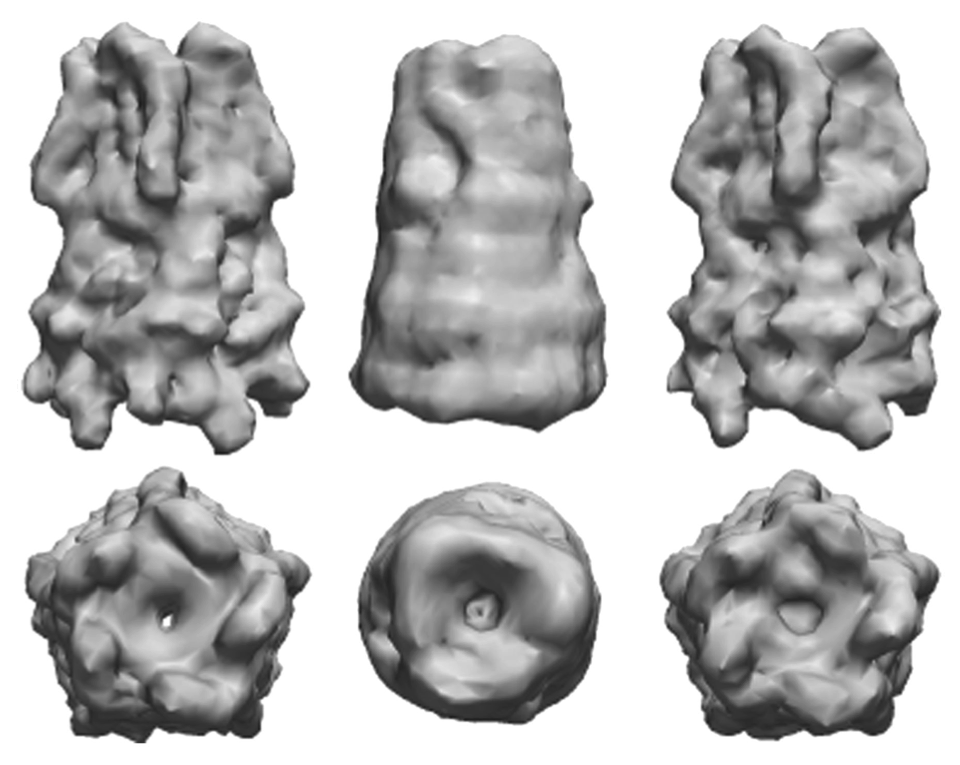
\includegraphics[width=.9\textwidth]{Don}
\caption{Electron density of a biomolecule as reconstructed directly from  the data in a PDB file in the left-hand column, and from the simulated XFEL Diffraction patterns on the right\cite{Donatelli}.}
\label{fig:Don}
\end{figure}

Since the structure of a protein depends very much on whether or not it is in a hydrated environment, we use a method of delivery of hydrated proteins to an XFEL within a solvent droplet of a few microns in size. It assumed that beam vaporizes the protein and droplet, but this does not matter in a “diffract-and-destroy” experiment \cite{Neutze} as it produces a diffraction pattern before then. If the background is constant, an argument due to Babinet \cite{babinet} may allow us to take account of the water scattering easily. Babinet  pointed out that of you add or subtract a constant density, it does not affect the sideways scattering only the intensity normally lost in the beam stop. That what is normally estimated by allowing these intensities to float in an iterative phasing algorithm or by constraining these intensities by the known molecular weight of the protein. If you subtract out exactly the value of the (constant) solvent density you would be assuming the scattering is by entities suspended in a vacuum but the electron densities of the entities had to be reduced by the solvent density. At least in the case of viruses, it has been possible to derive the structure from experimental data under this assumption. If it is possible to derive structure routinely from XFEL diffraction patterns which at the LCLS are measured at about 120 per second, then the possibility exists of measuring perhaps a million per experimental shift. The aim is to develop a method of extracting structural information from this data, to routinely solve the structures of biomolecules from the data. The XFEL unlocks the possibility of studying the structure of uncrystallized biomolecules \cite{Neutze}. Simulations show that molecules explode caused by intense brightness of the X-ray radiation after 50 femtoseconds beyond the initial incidence of the X-ray pulse \cite{Neutze}. However, meaningful diffraction patterns can be recorded before molecules explode because the pulse produced by the XFEL is significantly shorter than the time needed for the molecular explosion.

It should be emphasized that the diffraction patterns measured at an XFEL are initially from particles whose orientations are unknown. In usual X-ray crystallography the orientations of the entities whose structure one intends to find are known. Perhaps inspired by these methods, initial methods proposed for the XFEL aimed to find the relative orientations of the particles. This is often difficult to achieve unless there is a single particle in the beam. Consequently “hit-finder” methods \cite{cheetah} have to be developed that reject diffraction patterns from multiple particles. One problem with this approach is that the vast majority of droplets containing biomolecules are not used in the analysis. Indeed, John Spence, the Scientific Director the bioXFEL group believes this this to be the greatest single impediment to structure determination, due to the wasted proteins that are discarded \cite{spenceP}.

A method was proposed originally by Zvi Kam \cite{kam1978} to obtain information of structure by correlating two points in each diffraction pattern and averaging over all diffraction patterns. This is completely logical in any circumstance where the orientations of the particles are unknown as the angular correlations do not depend on orientation in the same way that the usually measured intensities of scattering do not depend on particle position (and so the structure may be deduced from the intensities independent of particle position). Likewise, from the angular correlations, the structure can be deduced independent of particle orientation.

It is true that the number of particles whose diffraction patterns are sought will vary from shot to shot. However, this is of no relevance as one will form the pair correlations and triple correlations [8]
\begin{eqnarray}
C_{3}(q,q',\Delta \phi) &=& \int I^{2}(q,\phi) I(q',\phi+\Delta \phi)  d\phi
\end{eqnarray}
from exactly the same set of diffraction patterns. What is more, the pair and triple correlations will be identical in form independent of the number of particles. All that matters is that exactly the same set of diffraction patterns are used for the pair and triple correlations, which is easily enough arranged.

Crystallography is a method for determining structure of the molecular constituents of crystals \cite{Drenth}. X-rays hit large numbers of identical molecules arranged in a crystal and Bragg spots appear as a result of interaction interference between the scattered X-rays. The intensities of the Bragg spots can be used to deduce the electron density of the molecule. The recovered density will be in a crystallized state whereas by using the XFEL, molecules are shot in their noncrystalline state. By studying molecules in their noncrystalline states, one may gain further insight into how they function in nature. 

Since individual biomolecules are studied in an XFEL, such objects have no translational symmetry and have no Bragg spots. What is more, as we have pointed out before, even their orientations are unknown. Despite this, we show that it is possible to deduce the structure from the collection of diffraction patterns measured in an XFEL. What is more, the angular correlations when integrated over all orientations are identical for all particles, Consequently, when a method is derived for reconstructing a structure from its correlations one should be able to deduce the structure of an individual molecule, even if a particular ensemble consists of many randomly oriented molecules \cite{kam1978}. We look in detail in this dissertation at the capabilities of the method of angular correlations. The reconstruction was done by simulating diffraction patterns from different random orientations of a virus that is known to have icosahedral symmetry \cite{saldinvirus} that is by simulating diffraction patterns known to be measurable in an XFEL. It should be stressed that all this method needs is a collection of diffraction patterns of random particle orientations. The flexibility of the method may be judged by the fact that it works just as well with diffraction patterns measured in the LCLS’s Single Particle Initiative (SPI) \cite{Munke} as with ensembles of randomly oriented particles that are probably inevitable with smaller molecules with a 1000 Angstrom wide XFEL illumination area. it is assumed that the diffraction volume has icosahedral symmetry. Another important point is that by taking symmetry into account it will greatly reduce the number of independent parameters to construct the diffraction volume due to the fact that information on orientations of the particle is unknown. 

Having information about the symmetry of particle is valuable. When transformed by a Legrendre function  $P_{l}$, the pair correlations. $C_{2}$ gives rise to a quantity $B_l$ that depends on the angular momentum quantum number $l$ \cite{PoonFiber}. It is possible to use the information contained in $B_{l}$ (and $T_{l}$ a similar transform of $C_3$) to deduce the magnitudes and signs of spherical harmonic coefficients of the diffraction volume characterized by l but not by the magnetic quantum number m \cite{Casper}. Until recently, information about m has to be deduced by the known symmetry of the particle As a result of this work at least the number of m values may be found from the $B_l$'s (derivable from experiment by singular value decomposition). Also the recent, as yet unpublished work of Donatelli, Saldin, and Zwart suggests a method of finding the full \Ilm coefficients from the correlations.

While on the subject of the Single Particle Initiative \cite{Munke}, this is an attempt at the LCLS to collect XFEL data from single molecules, but of all possible orientations to within a Shannon angle (The Shannon angle is defined as roughly the width of a single feature in  a diffraction pattern). In order to facilitate experiments that hit single particles, initial experiments have been on large bioparticles such as viruses. Consequently, we applied our method to experiments with the so-called rice dwarf virus (RDV) \cite{Munke} conducted at the LCLS in August 2015. The results are shown here. This shows a computer reconstructed image with a computational slice made to indicate whether or not there is genetic material on the inside. Our image correctly showed the genetic material inside unlike a structure reconstructed (also shown) from the data in the Protein Data Bank where the internal genetic material was removed.
Luckily, for a symmetry based method, for the two main categories of regular virus the icosahedral \cite{saldinvirus} and helical \cite{PoonFiber} a knowledge the symmetry allows a complete solution. The symmetry is an assumption taken in order to fill missing steps of the reconstruction. We have already seen that a knowledge of a particle’s symmetry is of great help in determining some of the crucial quantum numbers in the angular momentum description. Ideally one would like to determine these symmetry parameters from the experimental data rather that by assumption. We how in this dissertation that this is indeed possible by a singular value decomposition of quantities Bl deducible from the angular pair correlations.

From a study of angular correlations \cite{saldinvirus}, virus structure can be reconstructed by constraining intensity to be always positive. Under icosahedral symmetry, only signs of spherical harmonics expansion of diffraction volume are not unique from the $B_l$’s and a positivity constraint is suitable to resolve the signs. It will be shown in this dissertation that a positivity constraint can be used to determine intensity from matrix B by an optimization method thus enhancing the constraint to be used not just in icosahedral symmetry but also for different types of symmetry. For example, Caspar and Klug once said \cite{Casper} all regular viruses fall into the symmetry classes of icosahedral or helical so there are in any case not many symmetries to be tried. It would be helpful if these symmetries are deduced directly from the data and not left to trial and error.

Although the method of correlations is useful for getting more information from situations where one only has incoherent data, it is also useful for coherent XFEL radiation for a disordered array.
\begin{figure}[ht]
  \centering
  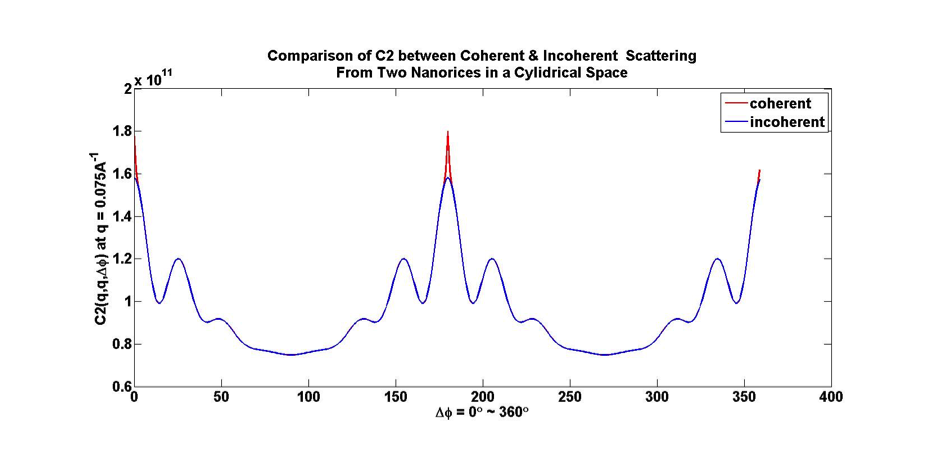
\includegraphics[width=1\textwidth]{kimplot}
\caption{Coherent peaks in (in red) in the correlations from incoherent diffraction patterns from the contributions of two independently randomly oriented nanoparticles, because the disorder gives rise to a kind of incoherence (except for narrow regions of reciprocal space that can easily be ignored \cite{kimmedicine}}
\label{fig:kimmedicine}
\end{figure}
What we mean is that in the presence of multiple particles one needs to look at correlations between particles as a result mutual interference. Quite simply, in the presence of two particles in a source of coherent radiation such an XFEL one would expect the total intensity to be $|\sum_{j=1} F_j \exp⁡(i\vec{}q\cdot\vec{r_j})|^2$ where $F_j$ is the structure factor of the jth molecule. The exponentials give rise to a factor of $\exp⁡(i\vec{q}\cdot(\vec{r}_j-\vec{r}_k )$) which results in random phases if the particle positions are random except that as $q\rightarrow 0$, when all phase factors become zero and are thus not random. Thus over most of its range one would expect interference fringes perpendicular to $\vec{r}_j-\vec{r}_k$  if the radiation is coherent. Fortunately, for different atom pairs, these fringes are random in orientation and spacing which makes the sum of cross terms amongst different particles tend towards zero, making the radiation effectively incoherent, over most of the q range as pointed out
before. It would be of interest though if the interference fringes exist. This is precisely what is observed in Figure \ref{fig:dpkim}. 
\begin{figure}[ht]
  \centering
  \includegraphics[width=0.9\textwidth]{dpkim}
\caption{Two particles illuminated simultaneously. If the radiation is coherent, one will see interference fringes, which will average out of there are many particles of random position.}
\label{fig:dpkim}
\end{figure}

While on individual diffraction patterns, fringes due to interference between the two particles are visible, the randomness of particle positions means that on different diffraction patterns these fringes will be in random directions and of random spacings. Consequently. when one adds contributions from different particles of random positions, the fringes essentially average out and it is if the sum is incoherent. That is, it is as if one were summing patterns like that in the bottom left above. Due to the randomness of the phases one may ignore the second summation over most of the $q$ range and therefore over most of the range one obtains what one would be equivalent of the incoherent sum $\sum_{j} I_j$ where $I_j$ is the intensity scattering contribution from particle $j$. Thus the total intensity reduces to a sum of intensity contributions from particle $j$, as if the scattering was not coherent \cite{kimmedicine}. The only exception occurs near $\Delta \phi =0$ (see Fig. \ref{fig:kimmedicine}, and equivalently $\Delta \phi =\pi $ due to Friedel symmetry, and $\Delta \phi = 2 \phi$ (same as $\Delta \phi =0$). These peaks are due to the fact that near $\Delta \phi =0$, all scattering phases become equal (and equal to zero). Thus the assumption of random phases is no longer valid. However, the width of such a peak is of the order of $2 \pi/L$ where $L$ is the width of the coherent radiation (about $L=1000$ \AA at the LCLS). Thus $2 \pi /L$ is usually much smaller than the width of a Shannon pixel $\pi /D$ where $D$ is of the order of $50$ Ang. Thus, in calculating $B_l$  or $T_l$  by integration under the curves of $C_2$ and $C_3$, respectively, can ignore the sharp high coherent peaks and still get essentially the same result. Thus the conclusion is for the present application of the reconstruction of the electron density of a biomolecule or virus from XFEL coherent radiation, these narrow peaks can be neglected, and the previous theory \cite{saldin2009} that applies also the single particle experiments like in the Single Particle Initiative \cite{Munke} is applicable.
\begin{figure}[ht]
  \centering
  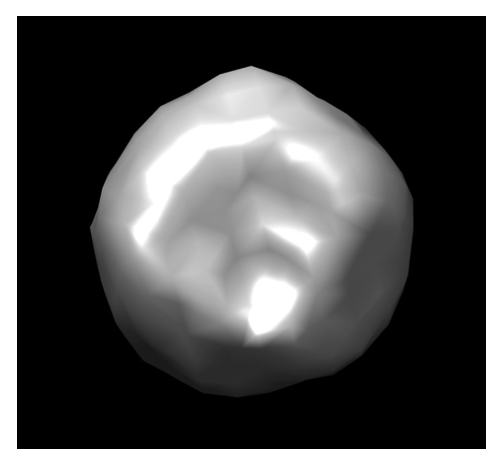
\includegraphics[width=0.7\textwidth]{kimvirus}
\caption{The rice dwarf virus (RDV) 
reconstructed from experimental data from 
the Single Particle Initiative measured in August 
2015. Note the apparent existence of internal 
genetic material, as the viruses in this 
experiment did not have the internal genetic 
material removed
}
\label{fig:kimvirus}
\end{figure}

\begin{figure}[ht]
  \centering
  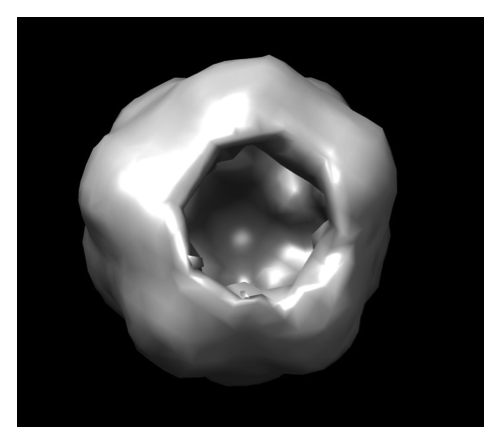
\includegraphics[width=0.7\textwidth]{kimvirus2}
\caption{
Similar image of the satellite tobacco 
necrosis virus whose structure in deposited in 
the protein data bank. This has had its internal 
genetic material removed, as revealed by the 
reconstructed image
}
\label{fig:kimvirus2}
\end{figure}

The method of angular correlations is also of great help with helical viruses \cite{PoonFiber}. In the past it has been attempted to study these entities by aligning them as in a fiber by physical means such was powerful electric fields. This has always run up against the obstacle of the entropic tendency to misalign.

Since the orientation of the reconstructed image may be chosen arbitrarily this allows an opportunity to use of the correlation method to align helical viruses computationally. It is usually assumed that the diffraction volume may be characterized by a magnetic quantum number $m=0$ if the z-axis can be taken along the helix. It turns out that even if the helices are randomly oriented in practice  merely choosing $m=0$ for the spherical harmonic components of the pair correlations $B_l$, computationally aligns the helical viruses and allows an estimate of the values of the spherical harmonic expansion coefficients of the diffraction volume \cite{PoonFiber}. Even if this is regarded as an approximation, the perturbation method we have developed for time-resolved structure \cite{pande2014} is capable of refining the values.

\begin{figure}[ht]
  \centering
  
\includegraphics[width=0.5\textwidth]{kimnano}
\caption{
Single particle of nanorice 
reconstructed from diffraction patterns of two 
independently randomly oriented particles.
}
\label{fig:kimnano}
\end{figure}

A real advantage of our method over all others that have been proposed for this problem is that it reconstructs the image from its correlations, Since the angular correlations of randomly oriented particles are identical, one can reconstruct an image of a single particle from an experiment consisting of multiple randomly oriented particles. Since the angular correlations are the same, independent of particle orientations, a corollary is that it may be reconstructed in any orientation. In general, an orientation is chosen to be consistent with the representation of the particle. An image of a single particle of nanorice reconstructed from diffraction patterns of two randomly oriented particles is shown next. 
In the case of a helical virus or a particle of nanorice, the diffraction volume is assumed to be azimuthally symmetric and m=0 is the only permitted component of the magnetic quantum number. (It should be emphasized that this is only possible because of the property of angular correlations as being the same independent of the particle orientation.)

With a focal spot of 1000 Angstrom, it is quite hard to focus on a single particle, and most diffraction patterns of proteins will probably be from multiple particles. It is true that one may remove diffraction patterns from multiple particles by so-called hit finder methods. But this is only at the expense of hit rate, as we have commented earlier 

It should be mentioned that, as currently formulated, the quantities $B_l$ and $T_l$ derived from $C_2$ and $C_3$, respectively, depend only on the azimuthal quantum number $l$. whereas the general the spherical harmonic expansion coefficients of the diffraction volume are characterized by both $l$ and the magnetic quantum number $m$. Consequently, it was proposed for both icosahedral and helical viruses that one uses the known symmetry properties for deducing the value of $m$ \cite{kam1978}. 

Ideally of course one may need to apply this method to completely non-symmetric particles. It has recently been shown to be possible to obtain spherical harmonic coefficeints $I_{lm}(q)$ characterized by particular values of $m$ by using the fact the so-called 3-point triple correlations. One first calculates the $I_{m}(q)$ coefficients of a circular harmonic expansion of the projections the structure using the method of Kurta et al. \cite{kurta} and Pedrini et al. \cite{pedrini}. Of course as one goes to lower X-ray energies one can exploit the increasingly curved nature of the Ewald sphere to get information on the $I_{lm}(q)$ coefficients of the 3D diffraction volume by an experiment like one on a “black-lipid membrane”. This will be no problem for membrane proteins which like to live within a membrane anyway. Since one of the stated aims of XFEL work is to determine the structure of hard-to-crystallize membrane proteins this a fulfillment of one of the original  aims of the construction of a nearly billion dollar XFEL.

We should also mention here other advantages of an angular momentum method particularly for icosahedral structures. Of the angular momenta $l$, while $l=0$ obviously has icosahedral symmetry, the next higher value of $l$ consistent with this symmetry is $l=6$. Consequently, if $B_l$ values are found from experimental data, the lower $l$ values should be dominated by $l=0$ and $l=6$. Thus even without an assumption of icosahedral symmetry one can get some indication of such symmetry form the experimental data even without a reconstruction of the particle’s image in real space. An example of such a calculation is shown below.

\begin{figure}[ht]
  \centering
  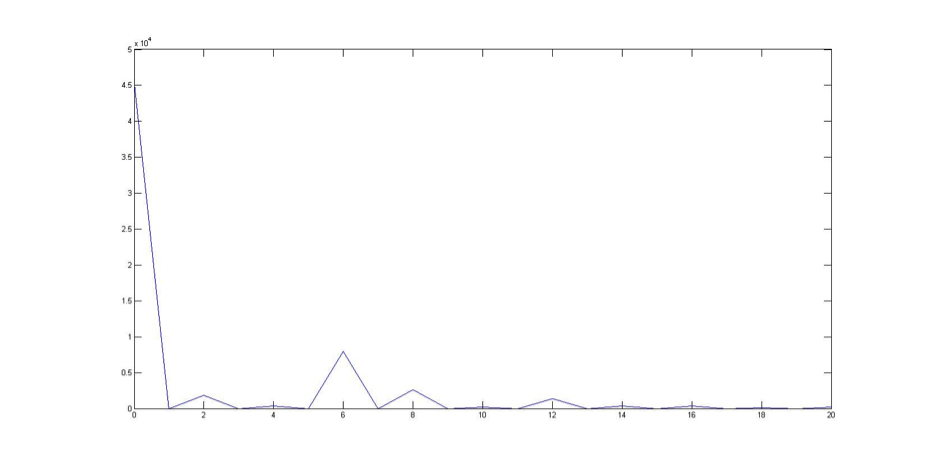
\includegraphics[width=1\textwidth]{kimBl}
\caption{
Calculation of the values of $B_l$ from experimental diffraction data from the rice dwarf virus without any symmetry assumption. This is dominated by $l=0$ and $l=6$,  a signature of icosahedral symmetry.
}
\label{fig:kimBl}
\end{figure}

Another advantage concerns the values of the intensity in the beam stop. There are less and less angular momenta as the scattering angle is reduced, In fact it can be shown that the maximum value of $l$ associated the outer edge of the beam stop is about 5. Since the maximum angular momentum associated with a given radius on a diffraction pattern is proportional to the radius and given that fact that the next lower angular momentum value consistent with icosahedral symmetry is $l=0$ one can estimate the intensity inside the beam stop if one has an analytic expression of the intensity that is angularly symmetric. In fact the known analytic form of the intensities from a uniform sphere of scattering matter is angularly symmetric, and it can be assumed to be the analytic extension of the computed intensities at higher scattering angle. This can be used to extend some of the intensities into the beam stop provided one ensures that the radial part of the data are continuous between the outer computational part and the inner analytic part. Indeed flipping-based phasing algorithms \cite{oszlanyi2004,oszlanyi2005} are often  very sensitive to the extent of the beam stop, and the extension of the data by this means is often of great help with a phasing algorithm.

%------
%Determination of molecular shape function,
%keeping all shape constant function
%Only vary the boundary
%Only use information of B zero
%The I0 enough for determinining the shape
%minimizing cost function
%I0 is independence of angular momemtun block
%------
%Time resolved structure,
%Two different structure,  
%----
%single axis random orientation
%the purpose to get the projected electron density 
%can be used to obtain nanorod 


% CHAPTER 2 Section X-Ray Diffraction
\chapter{Theoretical Foundation}
\section{X-ray Diffraction}
\begin{figure}[ht]
  \centering
  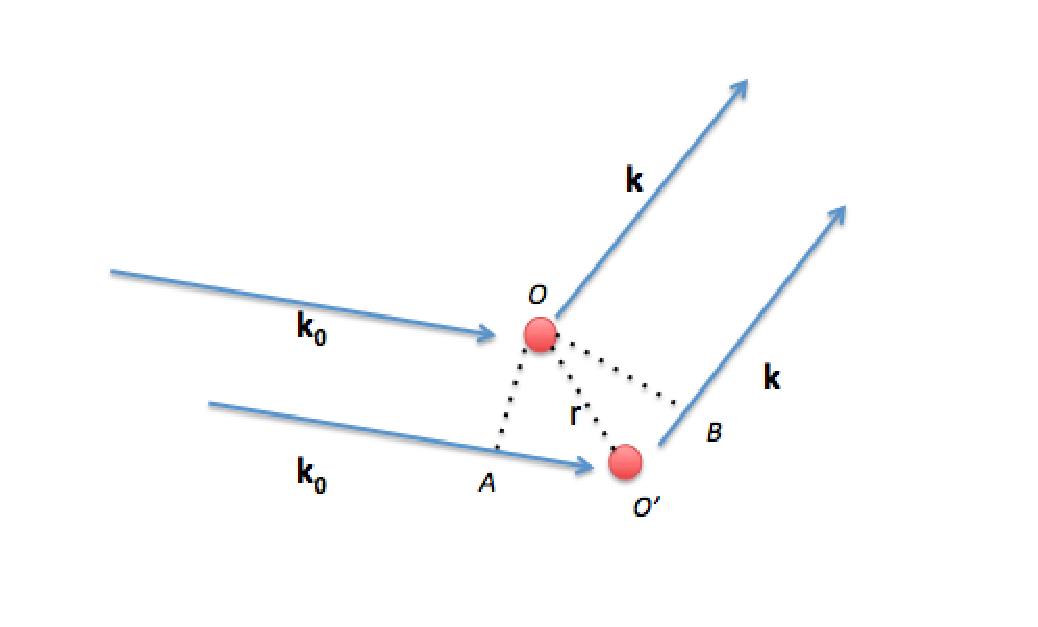
\includegraphics[width=.8\textwidth]{xraydiff}
\caption{Diagram of X-ray diffraction}
\label{fig:xraydiff}
\end{figure}
The diagram in Figure \ref{fig:xraydiff} shows the relation between the incoming waves, the scattered waves and the phase difference. The incoming wave that has wave vector $\vec{k_{0}}$ hits two electrons and they are scattered with the direction of $\vec{k}$. The scattered waves are parallel each other under approximation the observer is very far.

Because the scattered waves are scattered at different positions, the scattered waves will have a phase difference. Another way to see this, the phase difference arise because each scattered waves travel a different length. From figure 1, the bottom wave travels longer than the top wave so that there is a difference in path length.
From figure \ref{fig:xraydiff}, the difference in path length is
\begin{equation}
\mbox{Path difference}=\mbox{AO'}+\mbox{O'B}.
\end{equation}
AO' is projection of $\vec{r}$ along $\vec{k}_{0}$ and has length $\vec{r} \cdot \vec{k}_{0} $. On the other hand, O'B is negative projection of $\vec{r}$ along $\vec{k}$ and has length of $\vec{-r}\cdot \vec{k}$. The total path difference is $\vec{r} \cdot (\vec{k_{0}}-\vec{k})$ or $\vec{r} \cdot \vec{q}$ where $\vec{q}$ is $(\vec{k_{0}}-\vec{k})$ . The total phase difference become $\exp(2 \pi \vec{r} \cdot \vec{q})$.

The diffraction multiplies the amplitude of the scattered wave by a phase factor $\exp(2 \pi \vec{r} \cdot \vec{q})$. If there are many electrons with density $\rho(\vec{r})$ then the effect at particular point $\vec{q}$  will sum to
\begin{eqnarray}
A(\vec{q})=\int \rho(\vec{r}) \exp(2 \pi i \vec{q} \cdot \vec{r}) d \vec{r}.
\label{eq:ftransform}
\end{eqnarray}
So the structure factor appears as a Fourier transform of the electron density. The diffraction experiments only measure the square of absolute value of $A(\vec{q})$, which shows up as the intensity corresponding to $\vec{q}$. Mathematically, the intensity can be written as
\begin{eqnarray}
I(\vec{q})=|A(\vec{q})|^2. 
\label{intensquare}
\end{eqnarray}

There is a more convenient way to calculate a structure factor of the molecule rather than perform Fourier transform of its full electron density. The structure of the molecule can be decomposed into its individual atoms. As already known, there are many the same type of atoms inside the molecule but they differ in positions only. By knowing the Fourier transform of a single type of atom, it leads us to have easier computation because the total structure factor is a sum over all contribution of the Fourier transform of atoms in all position. Thus, calculating the Fourier transform of a single atom enables one to perform easier simulations to calculate structure factors.

The Fourier transform of a single atom is called atomic form factor. Based on a work done by Don Cromer and Mann \cite{CromerMann}, the Hartree-Fock approximation can be used to obtain empirical parameters to approximate atomic form factors. The way they determined the parameters was by fitting 9 parameters in a Gaussian function to a normalized scattering curves. Currently, those parameters are readily available from the international table of crystallography \cite{tablecryst} and the Gaussian function is shown in equation \ref{eq:cromcoef}. 

\begin{center}
  \begin{tabular}{| c | c | c | c | c | c | c | c | c | c | }
    \hline
    atom & $a_1$ & $a_2$ & $a_3$ & $a_4$ & $b_1 $& $b_2$ &$b_3$&$b_4$&$c$ \\ \hline
    C & 2.31 & 1.02 & 1.589 & 0.865 & 20.84 & 10.21 & 0.569 & 51.65 &0.216 \\ \hline
    N & 12.213 & 3.132 & 2.013 & 1.166 & 0.006 & 9.893 & 28.997 & 0.583 &-11.529 \\ \hline
    O & 3.049 & 2.287 & 1.546 & 0.867 & 13.277 & 5.701 & 0.324 & 32.909 & 0.251 \\ \hline
S & 7.070 & 5.340 & 2.236 & 1.512 & 1.366 & 19.828 & 0.092 & 55.228 & -0.159 \\ \hline
  \end{tabular}
\captionof{table}{Table of Cromer-Mann coefficients}\label{tab:ccMco}
\end{center}
\begin{figure}[ht]
  \centering
  \includegraphics[width=.8\textwidth]{atomicff}
\caption{Plot of atomic form vector for carbon and oxygen}
\label{fig:atomicff}
\end{figure}
The parameters for different type of atoms are listed in table \ref{tab:ccMco}. There are 9 parameters for each atom and the table shows only entries for carbon, oxygen, nitrogen, and sulfur. After knowing all 9 parameters, the atomic form factor can be calculated using Gaussian function:
\begin{equation}
f(\sin(\theta)/\lambda)= \sum_{i=1}^{4} a_{i} \exp(-b_{i}(\sin(\theta)/\lambda)^2)+c. 
\label{eq:cromcoef}
\end{equation}
 A plot of the atomic form for carbon and oxygen is shown in figure \ref{fig:atomicff}. It is shown in the plot that the value of atomic form factor goes to their atomic number when $\sin(\theta)/\lambda$ close to zero.

The structure factor can be calculated in a simpler way if the approximation of atomic form factor is used. Because the atomic form factor is calculated once, the calculation of the structure factor is done faster for all atoms. Finally, the expression for the structure factor in terms of the atomic form factors is described as
\begin{equation}
A(\vec{q})=\sum_{i} f_{i}(q) \exp(2 \pi \vec{q} \cdot \vec{r_i}). 
\label{eq:strfac}
\end{equation}

The equation \ref{eq:strfac} will be used to simulate structure factors for a molecule. As long as a molecule is listed as a collection of atoms in different positions, then equation \ref{eq:strfac} can be used to simulate the structure factor. Some structures of molecules have been solved using methods of crystallography and their structures are available in the protein data bank (pdb). The pdb file describes a molecule as a list of atom type as well as their positions. Having said that, one can simulate a structure factor by using equation \ref{eq:strfac} where the entry is from the pdb file.

\begin{figure}[ht]
  \centering
  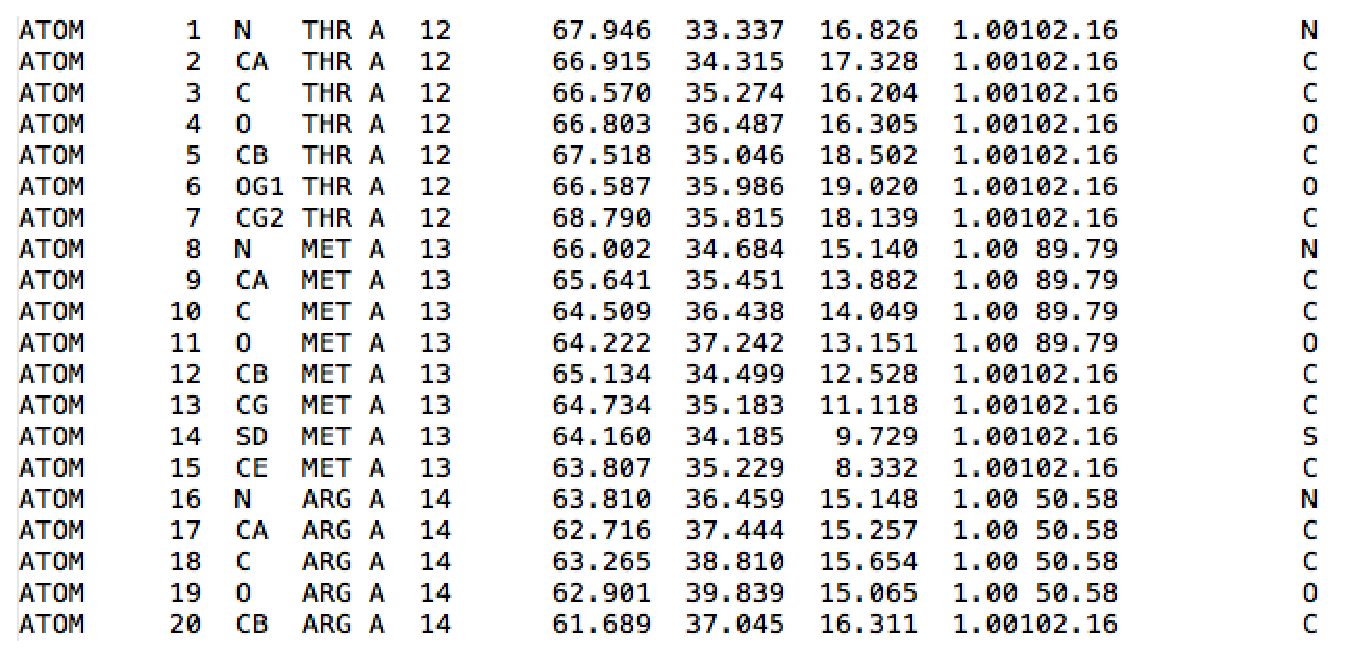
\includegraphics[width=.8\textwidth]{pdbshot}
\caption{Example of data from protein data bank in pdb format}
\label{fig:pdbshot}
\end{figure}

Figure \ref{fig:pdbshot} is a snapshot of a part of the pdb file. In order to read the information from pdb file, one requires to understande thoroughly the format and the convention of the file. First, the pdb file has row entries where each row is a single atom in particular position together with additional information. It consists of multiple columns where each column has particular information. In total, there are 27 columns and all data is in a text file in ASCII format. 

For the purpose of simulating the structure factors, only atom types and their positions are needed. Thus, there are four pieces of information needed, namely atom type, position-x, position-y, and position-z. The atom type is shown between columns 13 to 16. The position-x is shown between columns 31-38. The position-x is shown between columns 39-46. The position-x is shown between columns 47-54. With the information above, the structure factor can be simulated using equation \ref{eq:strfac} with the source of a pdb file. Full explanation about the format of pdb file is given in appendix \ref{ch:pdb}

\section{Angular Correlation} \label{sec:angcor}
\begin{figure}[ht]
  \centering
  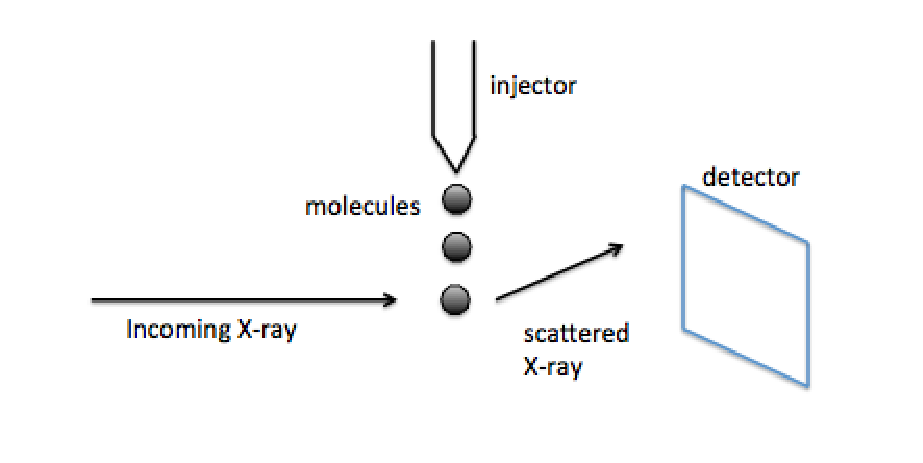
\includegraphics[width=.8\textwidth]{schemadifdes2}
\caption{Diagram of single particle diffraction experiment}
\label{fig:spiexp}
\end{figure}
A single particle diffraction experiment is an experiment that diffracts individual biomolecules using high intensity X-rays without crystallization. Figure \ref{fig:spiexp} shows the schematic design of the experiment.  The incoming X-ray produced in LCLS has high enough intensity so that detector can capture the scattered waves. The injector is capable to stream the molecules in tiny diameter so that there is chance an X-ray will hit a single molecule. 

The information obtainable from this setup is the diffraction patterns of the molecules. However, there is missing information from the setup, namely the information about the orientations of the molecules. Each diffraction pattern recorded by detector is very noisy therefore can't be used for information about the orientation of the molecules. It is important to note that the detector is able to record many millions of diffraction patterns. Although the information about the orientations is lost, it is still possible to get the information about the structure of the molecule by averaging many diffraction patterns. The next section explains the theory to reconstruct the structure of the molecules by averaging many random orientations of the diffraction patterns.  

\begin{figure}[ht]
  \centering
  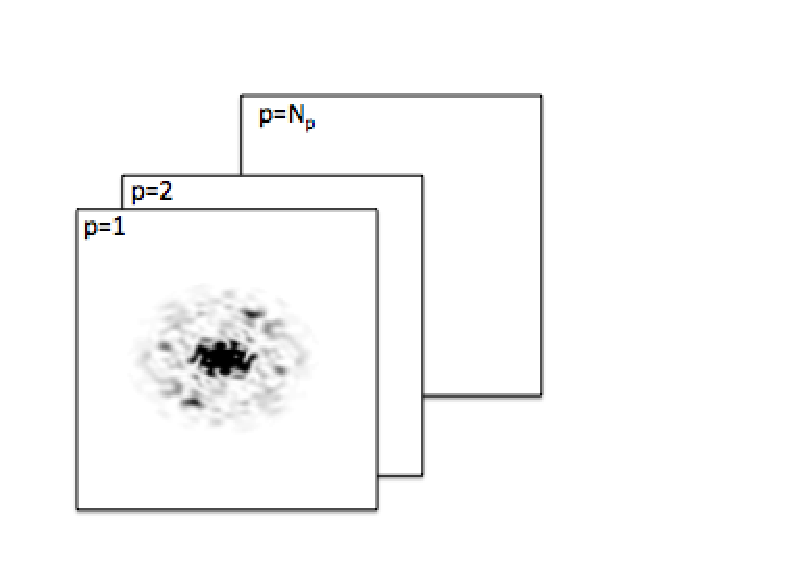
\includegraphics[width=.8\textwidth]{colldp}
\caption{Collection of random angle diffraction patterns}
\label{fig:colldp}
\end{figure}
Figure \ref{fig:colldp} illustrates typical outputs of a diffract and destroy experiment. The output consists of a collection of the diffraction patterns in random orientations. In order to remove the angular dependence, we need to take average over all diffraction patterns. Because the structure of molecule cannot be obtained by only taking average of a point in the diffraction patterns as all point average to the same for random molecules orientations, two points averaging is done to obtain more information about the structure of molecules. The final goal is to derive an angle independent quantity, which has information about the structure, by correlating two points in the diffraction patterns and summing over all diffraction patterns.
\begin{figure}[ht]
  \centering
  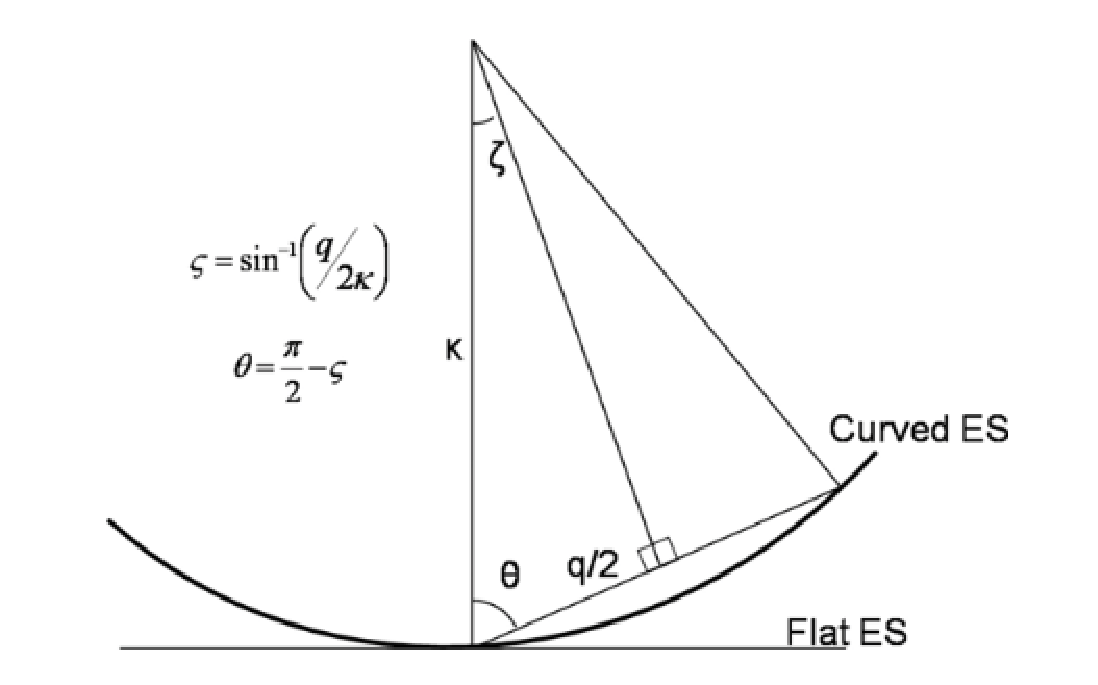
\includegraphics[width=.7\textwidth]{ewsphe}
\caption{Relation between reciprocal radial distance $q$ and angle $\theta$ in an Ewald sphere \cite{saldin2009} }
\label{fig:ewrelation}
\end{figure}

Before going into the derivation of correlations, it is important to derive relation between the intensity and the diffraction pattern. Figure \ref{fig:ewrelation} is a section through the Ewald sphere and a single diffraction pattern samples 3D reciprocal space in Ewald sphere. Consequently, one can derive the relation between the polar angle $\theta$ and the distance $q$, namely 
\begin{eqnarray}
\theta(q) = \frac{\pi}{2} - \sin ^{-1}(\frac{q}{2 \kappa})
\label{eq:thetarelationq}
\end{eqnarray}
as illustrated in figure \ref{fig:ewrelation}.

The curvature of Ewald sphere for arbitrary X-ray wave number $\kappa$ is taken into account correctly by expressing $\theta$ in terms of $q$ and $\kappa$. By substituting $\theta$ in equation \ref{eq:thetarelationq}, any point in a diffraction pattern can be specified by its $q$ and $\phi$ as illustrated in figure \ref{fig:polarcor}. Another step is by taking Z-axis as the direction antiparallel to the incident wave then the measured intensity in a diffraction pattern can be expressed as
\begin{eqnarray}
I_{Z}(q,\phi)=\sum_{lm} I_{lm} Y_{lm}(\theta(q),\phi).
\end{eqnarray} 

Figure \ref{fig:colldp} illustrates that there are many diffraction patterns and index $p$ corresponds to the diffraction patterns with different molecular orientations. The orientation can be seen as a rotation of frame of reference because a rotation of the molecule is equivalent to an inverse rotation of its frame of reference. Mathematically, the particular orientation can be expressed by applying rotation operator to its original basis function. Specifically, the rotation operator is matrix $D_{lm}$ because we chose spherical harmonics as basis function of intensity. Consequently, the new diffraction pattern in rotated frame of reference is  
\begin{eqnarray}
I^{(p)}(q,\phi)=\sum_{lmm'}I_{lm}(q) D^{(p)}_{lmm'}(\alpha,\beta,\gamma) Y_{lm'}(\theta(q),\phi).
\label{Idiffrot}
\end{eqnarray}

\begin{figure}[ht]
  \centering
  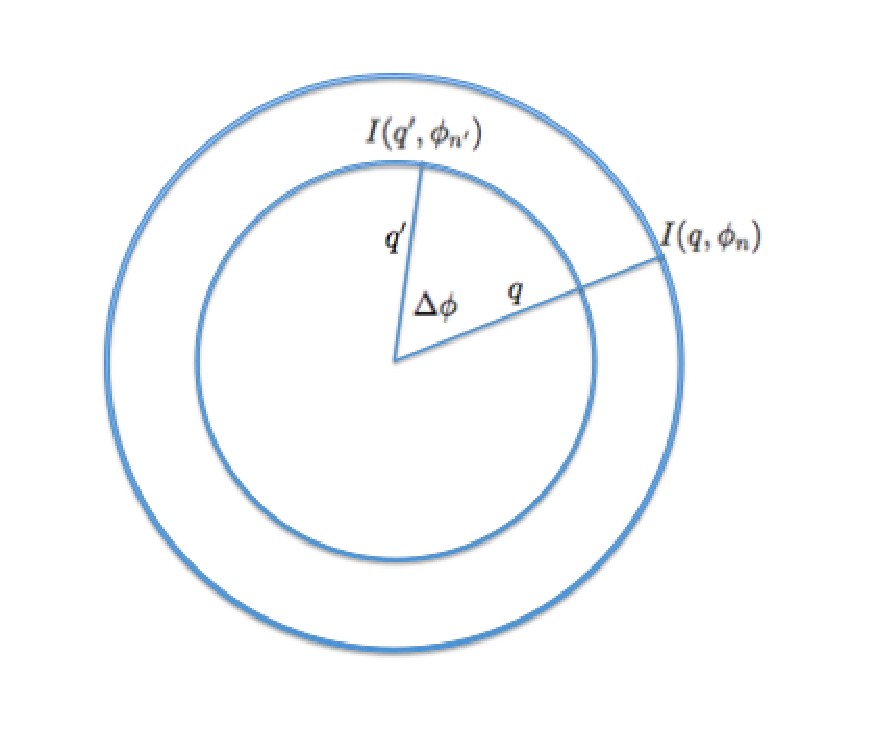
\includegraphics[width=.8\textwidth]{polarcor}
\caption{Two points correlation in a diffraction pattern}
\label{fig:polarcor}
\end{figure}

The first step in using this method is to calculate angular cross correlations on each diffraction pattern  in polar coordinates. Polar coordinates are natural for this problem since the particles differ mainly in their orientations (They may also differ in position, but this does not affect the diffraction pattern intensities that are insensitive to the particle phases).

As illustrated in figure \ref{fig:polarcor}, we can pick any two points in the polar diffraction pattern by specifying the coordinate $q$ and angle $\phi$.  The next step is to correlate every point in rings $q$ and $q'$ by keeping the same angular distance  $\phi$ and $\phi'$. Angular pair correlations are defined by
\begin{eqnarray}
C_{2}(q,q',\phi,\phi') &=& \frac{1}{N_{p}} \sum_{p} I^{(p)}(q,\phi) I^{(p)}(q',\phi') 
\label{eq:crosscor}
\end{eqnarray}
where $p$ is the index of the diffraction patterns and $N_p$ is the total number of diffraction pattterns as illustrated in figure \ref{fig:colldp}.

Equation \ref{eq:crosscor} can be expressed in terms of summation of points in diffraction patterns rotated by matrix $D^{(p)}_{lm}$. By substituting equation \ref{Idiffrot} into equation \ref{eq:crosscor}, the $C_{2}$ become
\begin{align}
\begin{split}
C_{2}(q,q',\phi,\phi') = \frac{1}{N_{p}} &  \sum_{p} \sum_{lmm'} \sum_{l'm''m'''}I^{*}_{lm}(q) D^{(p)*}_{lmm'} Y^{*}_{lm'}(\theta(q),\phi) \\
&\times I_{l'm''}(q) D^{(p)}_{l'm''m'''} Y_{l'm'''}(\theta'(q'),\phi') 
\label{eq:crossDangle}
\end{split}
\end{align}

The Wigner $D$-matrices are representation of the full rotation group. A set of the Euler angles specify the rotation of matrix $D$. Due to the randomness of the orientations of the diffraction patterns, the larger the number of diffraction patterns the most likely the angles will occupy the entire space. Under assumption that the set of random angles will converge into all uniform rotational angles then equation \ref{eq:crossDangle} can be simplified. The relation that is used to simplify the equation is called the orthogonality theorem, which mathematically expressed as
\begin{eqnarray}
\frac{1}{N} \sum_{(p)} D^{(p)*}_{lmm'} D^{(p)}_{l'm''m'''}=\frac{1}{2l+1} \delta_{ll'} \delta_{mm''} \delta_{m'm'''}.
\label{eq:orthotheorem}
\end{eqnarray}

By summing over $p$ in equation \ref{eq:crossDangle}, making use of the great orthogonality relation in equation \ref{eq:orthotheorem}, and then summing over $l'$, $m''$, and $m'''$ will transform equation \ref{eq:crossDangle} into 
\begin{eqnarray}
C_{2}(q,q',\phi,\phi') = \sum_{l} F_{l}(q,q';\phi,\phi') B_{l}(q,q')
\label{C2definition}
\end{eqnarray}
where
\begin{eqnarray}
F_{l}(q,q';\phi \phi') &=& \frac{1}{2l+1} \sum_{m} Y^{*}_{lm}(\theta(q),\phi) Y_{lm}(\theta'(q'),\phi') \\
&=&\frac{1}{4} P_{l} [\cos \theta (q) \cos \theta (q') + \sin \theta(q) \sin \theta(q') \cos(\phi-\phi') ]
\label{eq:FP}
\end{eqnarray}
where $P_{l}$ is a Legendre polynomial of order l, and
\begin{eqnarray}
B_{l}(q,q') &=& \sum_{m} I_{lm}(q) I_{lm}^{*}(q').
\label{eq:theB}
\end{eqnarray}
The left hand side of equation \ref{C2definition} is obtainable from experiment. The first term of right hand side of equation \ref{C2definition} can be calculated mathematically. Consequently, the quantity $B_{l}$ can be obtained from experiment and it can be used to get the information about the structure of the molecule.

The calculation to extract $B_{l}$ from equation \ref{C2definition} is matrix inversion. For each pair $q$ and $q'$, equation \ref{C2definition}  may be written as the matrix equation
\begin{eqnarray}
C_{2(\phi\phi')}=\sum_{l} F_{\phi\phi',l}B_{l}.
\end{eqnarray}
All elementes of matrix $F$ are real number. Thus, the above equation can be inverted to get real coefficients $B_{l}$ where
\begin{eqnarray}
B_{l}=\sum_{\phi \phi'} {F^{-1}}_{l,\phi \phi'} C_{2(\phi \phi')}.
\label{eq:Binvert}
\end{eqnarray}

The above equation can be used to calculate \Blq after $C_{2}$ is obtained. 
The information about the structure of the molecules is contained in \Blq because \Blq contain information about $I_{lm}(q)$ where $I_{lm}(q)$ are spherical harmonic expansion of a diffraction volume. Thus, the information about the structure of molecules can be obtained by calculating \Blq from a set of random angle diffraction patterns.

The spherical harmonics are used to expand the diffraction volume because it can construct any function in a 2D surface. In 3D case, a molecule is free to rotate in any two angles, namely azimuthal and polar angle. However, in 2D case only rotation with respect to single axis is allowed. Thus, a basis functions with single rotation is simpler to be used than spherical harmonics. 

Beside spherical harmonics, circular harmonics can be used to expand the intensity as long as the random angles only have a single axis. The expression of the diffraction patterns in terms of circular harmonic expansion can be written 
\begin{eqnarray}
I(q,\phi)= \sum_{m} I_{m}(q) \exp(im\phi).
\label{eq:Imq}
\end{eqnarray}
This is derived similarly as before, by substituting equation \ref{eq:Imq} into equation \ref{eq:crosscor} and performing the average over all diffraction patterns,the new $C_{2}$ with respect to circular harmonics become
\begin{eqnarray}
C_{2}(q,q';\phi \phi')=\sum_{m} I^{*}_{m}(q) I_{m}(q') \exp(im(\phi-\phi'))
\label{eq:c2Imq}
\end{eqnarray}
where \Imq is the circular harmonic expansion coefficients of the diffracted intensity of a single particle. The right hand side of equation \ref{eq:c2Imq} 
is an exponential function. By multiplying both side with its inverse and integrating over all angles, it will remove the dependence of the exponential function in the right hand side of the equation. Thus, a new quantity can be obtained, namely
\begin{eqnarray}
B_{m}(q,q')&=&\int C_{2}(q,q',\Delta \phi) \exp(-i m \Delta \phi) d\Delta\phi= I_{m}(q)^{*} I_{m}(q') \\
\label{eq:Bmqdef}
\end{eqnarray}

The information about the structure is contained in the quantity $I_{m}(q)$. The magnitude of $I_{m}(q)$ is directly accessible by taking square root of the diagonal values of \Bmq. For that reason, the phase of $I_{m}(q)$ is the only missing information to fully determine $I_{m}(q)$ from \Bmq. After $I_{m}(q)$ is determined, the reconstruction of the intensity distribution of a single molecule can be found from equation \ref{eq:Imq}. 

Now after deriving \Blq and \Bmq, there is another quantity that is very important for reconstruction of structure of the molecule, namely two point angular triple correlations. Mathematically, it is defined by \cite{kam1978}
\begin{eqnarray}
C_{3}(q,q',\phi,\phi') &=& \frac{1}{N_{p}} \sum_{p} I_{p}^{2}(q,\phi) I_{p}(q',\phi') 
\label{eq:crosstripcor}
\end{eqnarray}

Similar derivation as before, the expansion coefficients in equation \ref{Idiffrot} are substituted into equation \ref{eq:crosstripcor}. The result of substitution is
\begin{align}
\begin{split}
C_{3}(q,q',\phi,\phi') &= \frac{1}{N_{p}} \sum_{p} \sum_{l_{1},l_{2},l_{3}} \sum_{m_{1},m_{2},m_{3}} \sum_{m'_{1},m'_{2},m'_{3}} \\ 
&\times I_{l_{1}m_{1}} D_{l_{1}m_{1}m'_{1}}(\omega) Y_{l_{1}m'_{1}}(\theta,\phi) \\ 
&\times I_{l_{2}m_{2}} D_{l_{2}m_{2}m'_{2}}(\omega) Y_{l_{2}m'_{2}}(\theta,\phi) \\ 
&\times I^{*}_{l_{3}m_{3}} D^{*}_{l_{3}m_{3}m'_{3}}(\omega') Y^{*}_{l_{3}m'_{3}}(\theta,\phi' ). \\ 
\label{eq:c3subs}
\end{split}
\end{align}

To simplify the above equation, these relations are substituted into the above equation:
\begin{align}
\label{eq:triprel1}
\begin{split}
D_{l_{1}m_{1}m'_{1}}(\omega) D_{l_{2}m_{2}m'_{2}}(\omega)&= \sum^{l_1+l_2}_{L=|l_1-l_2|} \sum_{(M,M')=-L}^{L}(2L+1)(-1)^{M-M'}  \\ 
&\times\left( \begin{array}{ccc}
l_1 & l_2 & L \\
m_1 & m_2 & -M  \end{array} \right)  \\ 
&\times\left( \begin{array}{ccc}
l_1 & l_2 & L \\
m'_1 & m'_2 & -M'  \end{array} \right) D_{LMM'}(\omega), 
\end{split}
\end{align}

\begin{align}
\label{eq:triprel2}
\begin{split}
Y_{l_1 m'_1}(\Omega)Y_{l_2 m'_2}(\Omega) &= \sum_{\lambda=|l_1-l_2|}^{l_1+l_2} \sum_{\mu=\lambda}^{+\lambda} \left[\frac{(2l_1+1)(2l_2+1)(2l_1+1)}{4 \pi}\right]^{1/2} \\
&\times \left( \begin{array}{ccc}
l_1 & l_2 & \lambda \\
0 & 0 & 0  \end{array} \right)  \\ 
&\times \left( \begin{array}{ccc}
l_1 & l_2 & \lambda \\
m_1' & m_2' & \mu  \end{array} \right) Y_{\lambda\mu}(\Omega), \\  
\end{split}
\end{align}

\begin{align}
\sum_{m'_1 m'_2}\left( \begin{array}{ccc}
l_1 & l_2 & \lambda \\
m'_1 & m'_2 & \mu  \end{array} \right) 
\left( \begin{array}{ccc}
l_1 & l_2 & l_3 \\
m'_1 & m'_2 & -m'_3  \end{array} \right) 
=\frac{1}{2l_3+1} \delta_{\lambda l_3}\delta_{\mu m'_3}, 
\label{eq:triprel3}
\end{align}
and
\begin{align}
\sum_{m'3} Y_{lm'_3}(\theta,\phi) Y^{*}_{lm'_3}(\theta,\phi')=\frac{2l+1}{4 \pi} P_{l}(\cos(\phi-\phi')) 
\label{eq:triprel4}
\end{align}
where the quantities represented by the large parentheses are Wigner $3j$ symbols.

After substituting equations \ref{eq:triprel1}, \ref{eq:triprel2}, \ref{eq:triprel3}, and \ref{eq:triprel4} into equation \ref{eq:c3subs}, the equation \ref{eq:c3subs} become
\begin{align}
\begin{split}
C_{3}(q,q',\Delta \phi)&= \sum_{l_1 l_2 l} \sum_{m_1 m_2 m} I_{l_1 m_1}(q) I_{l_2 m_2}(q) I^{*}_{l m}(q') P_{l}(\cos(\Delta \phi)) \\ 
&\times (-1)^{m}(4\pi)^{-\frac{3}{2}} 
\left( \begin{array}{ccc}
l_1 & l_2 & l \\
m_1 & m_2 & -m  \end{array} \right) 
\left( \begin{array}{ccc}
l_1 & l_2 & l \\
0 & 0 & 0  \end{array} \right)  \\ 
&\times \left[(2l_1+1)(2l_2+1)(2l_1+1)\right]^{1/2}.
\end{split}
\label{eq:tripc3}
\end{align}

Additional relation is needed to invert the equation \ref{eq:tripc3}. The relation is orthogonality of the Legendre polynomials, the mathematical expression is
\begin{eqnarray}
\int_{-1}^{1} P_{l}(u) P_{l'}(u) du =\frac{2}{2l+1} \delta_{ll'}. 
\end{eqnarray}
A new quantity $T_{l}(q,q')$ is obtained by applying the orthogonality of the Legendre polynomials into equation \ref{eq:tripc3}. The $T_{l}(q,q')$ can be written as
\begin{align}
\begin{split}
T_{l}(q,q')&=\int C_{3}(q,q',\Delta \phi)  P_{l}(\cos(\Delta \phi)) d(\Delta \phi) \frac{(2 l+1)}{2} 4 \pi \\ 
\label{eq:tripleexp}
\end{split}
\end{align}
or theoretically can be calculated from
\begin{align}
\begin{split}
T_{l}(q,q')&= \sum_{l_1,l_2,m_1,m_2,m} (-1)^m
 \left[\frac{(2l_1+1)(2l_2+1)(2l_1+1)}{4 \pi}\right]^{1/2}
 \left( \begin{array}{ccc}
l_1 & l_2 & l \\
0 & 0 & 0  \end{array} \right) 
 \left( \begin{array}{ccc}
l_1 & l_2 & l \\
m_1 & m_2 & -m  \end{array} \right)  \\ 
&  I_{l_1,m_1}(q) I_{l_2,m_2}(q) I_{l,m}(q).       
\label{eq:triple}
\end{split}
\end{align}

Apart from \Blq, the information about the structure of the molecule can be obtained from $T_{l}(q,q')$ as well. The $C_{3}$ is a quantity that is obtainable from experiment data as described in equation \ref{eq:crosstripcor}. Thus, $T_{l}(q,q')$ can be calculated from experiment data as described in equation \ref{eq:tripleexp}. As a result of that, $T_{l}(q,q')$ can be used to reveal the information about the structure of the molecule because it involves the summation over spherical harmonics expansion of the diffraction volume.
\subsection{Independent Parameters}
As stated before, \Blq is one of the quantities measurable in the experiment. The objective of this method is to obtain the electron density from the \Blq. If the diffraction volume or intensity can be obtained from \Blq then the diffraction volume can be phased using a phasing algorithm to get the electron density. Having said that, it is important to study relationship between \Blq and \Ilm. 

For a given \Blq, \Ilm cannot be determined uniquely. The reason of that is a new \Ilm can be formed by multiplying it by orthogonal matrix. 
\begin{eqnarray}
I_{lm}'(q)=O^{l}_{mm'}I_{lm'}(q)  \\
\mbox{where} \quad O^{l}_{mm'} (O^{l}_{mm'})^{\dagger} =1. 
\label{eq:ilmolm}
\end{eqnarray}
In other words, if a matrix $O^{l}_{mm'}$ is unitary or orthogonal then the value of \Blq is not affected by multiplication of any orthogonal matrix as shown below:
\begin{eqnarray}
B_{l}'(q,q')&=&\sum_{m} I_{lm}'(q) I_{lm}'^{\dagger}(q') \\
B_{l}'(q,q')&=&\sum_{m} I_{lm}(q) O^{l}_{m'm''} (O^{l}_{m'm''})^{\dagger} I_{lm}^{\dagger}(q') \\ \nonumber
B_{l}'(q,q')&=&\sum_{m} I_{lm}(q)  I_{lm}^{\dagger}(q') \\ \nonumber
B_{l}'(q,q')&=&B_{l}(q,q'). \\ \nonumber
\label{eq:Blilmolm}
\end{eqnarray}

For each $l$, there are unitary matrices $O^{l}_{mm'}$ that contribute to the nonuniqueness of \Ilm. The matrices $O^{l}_{mm'}$ have $2l+1$ rows and $2l+1$ columns. The total elements of the particular matrix is $(2l+1)^2$. However, not all elements are independent of each other because the matrix satisfy orthogonality. 

From \cite{tinkham}, an $n \times n$ orthogonal matrix has $\frac{n(n-1)}{2}$ independent elements. Since an $O^{l}_{mm'}$ has $(2l+1)$x$(2l+1)$ elements then the total independent elements for a particular $l$ is $(2l+1)(l)$ elements. 

Given the explanation above, the total elements is
\begin{eqnarray}
\sum_{l=0,2,4,...}^{l_{max}} (2l+1)(l).
\label{eq:indcomp}
\end{eqnarray}


% CHAPTER 2 Section Spherical Harmonics
\section{Spherical Harmonics}
\subsection{Property of Spherical Harmonics}
As mentioned in the previous section, the correlation method doesn't need to know individual orientation of diffraction pattern. It is very crucial to remove angle dependence of intensity since we want to recover particle structure. It is important that the selected function can be separated by its angle dependence and radius dependence. A set of functions that satisfies such criterion are spherical harmonics.

Spherical harmonics are a series of special function defined on the surface of sphere. It is defined in spherical coordinates represented by angles $\theta$ and $\phi$. The angular property of spherical harmonics is characterized by two quantum number namely $l$ and $m$. Another quantum number is $m$ represents how a function varies with respect to azimuthal angle. 

\begin{figure}[h]
  \centering
  \includegraphics[width=.8\textwidth]{sphexample}
\caption{Example of plot of spherical harmonics with different quantum numbers }
\label{fig:sphexample}
\end{figure}

The definition of spherical harmonics is given by
\begin{eqnarray}
Y_{lm}(\theta,\phi)=\sqrt{\frac{2l+1}{4 \pi}\frac{(l-m)!}{(l+m)!}} P_{lm}(\cos \theta) e^{im\phi}
\label{eq:sphhar}
\end{eqnarray}
where $P_{lm}(\cos \theta)$ is legendre polynomials. Legendre polynomial $P_{lm}(x)$ can be obtained using Rodrigues formula:
\begin{eqnarray}
P_{lm}(x)=\frac{(-1)^m}{2^{l} l!} (1-x^2)^{m/2}\frac{d^{l+m}}{dx^{l+m}}\left[(x^2-1)^l\right].
\label{eq:rodfor}
\end{eqnarray}

It is important to note that spherical harmonics are a polynomial of trigonometric function. As in other polynomial expansion, lower degree represents approximation of the function and higher degree contain information of how rapid the function varies.  

Since spherical harmonics are a set of functions characterized by 2 quantum numbers, it is important to show relation between those functions. Every single spherical harmonics function with different quantum number are orthogonal or mathematically it is represented by
\begin{eqnarray}
\int Y_{lm} Y_{l'm'}^{*} d\Omega= \delta_{ll'}\delta_{mm'}
\end{eqnarray}
where $\delta_{ll'}$ is Kronecker delta that is non zero only if indices are the same. 

The aim of this section is to characterize a symmetry in terms of spherical harmonic quantum numbers. In order to study rotational symmetry, an operator of rotation in spherical harmonics basis is needed. One well known operator to rotate spherical harmonics is the Wigner D-matrix. Definition below shows how spherical harmonics are rotated,
\begin{eqnarray}
Y_{lm}(\theta',\phi')=\sum_{m'}D^{l}_{mm'}(\alpha,\beta,\gamma)Y_{lm'}(\theta,\phi)
\end{eqnarray} 
where $\theta$, $\phi$ are with respect to original axes and the $\theta'$, $\phi'$ are with respect to rotated relative to their Euler angles ($\alpha$,$\beta$,$\gamma$). Elements of the Wigner D-matrix are calculated as follows:
\begin{eqnarray}
D^{l}_{mm'}(\alpha,\beta,\gamma)=e^{im'\gamma}d^{j}_{mm'}(\beta)e^{-im\alpha}
\end{eqnarray}
and $d^{j}_{mm'}$ is calculated by applying summation:
\begin{eqnarray}
&&d^{j}_{mm'}(\beta)=[(j+m')!(j-m)!(j+m)!(j-m)!]^{1/2}\\ \nonumber
&&\sum_{s}\frac{(-1)^{m'-m+s}}{(j+m-s)!s!(m'-m+s)!(j-m'-s)!} \cos(\frac{\beta}{2})^{2j+m-m'-2s} \sin(\frac{\beta}{2})^{m'-m+2s} ]
\end{eqnarray}

Another important property of spherical harmonics is they can be representated in a real basis function. It is easier to determine the number of the independent parameters in the real spherical harmonics because there is only the real number for all spherical harmonics expansion. A real basis of spherical harmonics is defined
\begin{align}
\begin{split}
Y_{lm}&=\sqrt(2)(-1)^{m} \operatorname{Im}(Y_{l|m|}) \quad \mbox{if} \quad m<0 \\
Y_{lm}&=Y_{l0} \quad \mbox{if} \quad m=0 \\
Y_{lm}&=\sqrt(2)(-1)^{m} \operatorname{Re}(Y_{l|m|}) \quad \mbox{if} \quad m>0. 
\end{split}
\label{eq:realsph}
\end{align} 

\subsection{Effect of Azimuthal Symmetry on Spherical Harmonics Expansion}
\label{subsec:azimsym}
It is very essential to discuss the azimuthal symmetry of the spherical harmonics. One important feature is how coordinate transformation affects the expansion of spherical harmonics. It will be shown here how by rotating coordinate and by setting z-axis as the center of symmetry, some component of spherical harmonics vanish.

In figure \ref{fig:azimuthrot}, the z-axis is not aligned to the center of symmetry of the object. Even though the object is a cylinder, which has azimuthal symmetry, none of spherical harmonics components will be zero. The reason is that by rotating the object with respect to z-axis the symmetry requirement is not satisfied. Having said that, rotation of axes is very important to determine  how symmetry of object affects spherical harmonics expansion.
 \begin{figure}[h]
  \centering
  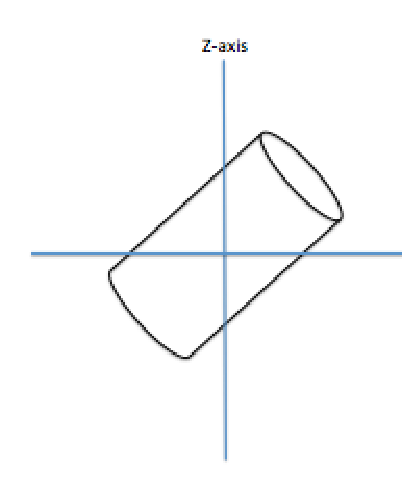
\includegraphics[width=.6\textwidth]{azimathrot}
\caption{Rotation of z-axis doesn't reveal azimuthal symmetry}
\label{fig:azimuthrot}
\end{figure}

In figure \ref{fig:azimuth}, the z-axis is now aligned to the center of symmetry of object. There is no change in appearance of object by rotation with respect to z-axis. Since symmetry is found in this coordinate transformation, there is pattern of m quantum number in spherical harmonics expansion.  
\begin{figure}[h]
  \centering
  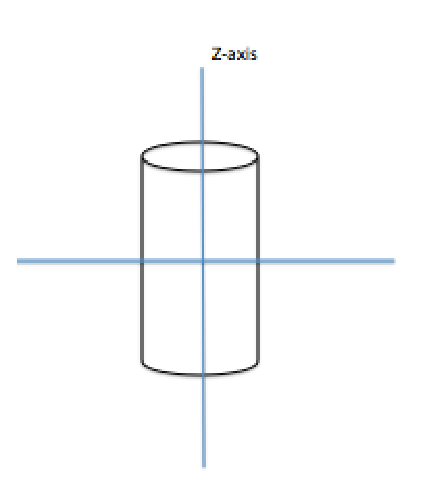
\includegraphics[width=.6\textwidth]{azimuth}
\caption{Rotation with respect to z-axis doesn't change the structure of object}
\label{fig:azimuth}
\end{figure}
By equating spherical harmonics before and after transformation,
\begin{eqnarray}
Y_{lm}(\theta,\phi)&=&Y_{lm}(\theta,\phi+\delta) \\ \nonumber
 Y_{lm}(\theta,\phi)&=&\sqrt{\frac{2l+1}{4 \pi}\frac{(l-m)!}{(l+m)!}} P_{lm}(\cos \theta) e^{im\left(\phi+\delta \right)} \\ \nonumber
\sqrt{\frac{2l+1}{4 \pi}\frac{(l-m)!}{(l+m)!}} P_{lm}(\cos \theta) e^{im\left(\phi \right)} &=& \sqrt{\frac{2l+1}{4 \pi}\frac{(l-m)!}{(l+m)!}} P_{lm}(\cos \theta) e^{im\left(\phi+\delta \right)} \\ \nonumber
e^{im\left(\phi\right)} &=& e^{im\left(\phi+\delta \right)}
\end{eqnarray}
$e^{im\left(\phi\right)} = e^{im\left(\phi+\delta \right)}$ is requirement to be satisfied if object has azimuthal symmetry with respect to z-axis. Since $\delta$ is any arbitrary angle, only $m=0$ satisfy the equation as it is shown in table \ref{tab:azim}
\begin{table}[h]
\begin{center}
  \begin{tabular}{ | c | c  |}
    \hline
    m & $e^{im\left(\phi\right)} = e^{im\left(\phi+\delta \right)}$  \\  \hline
    m=0 &\textcolor{red}{1=1} \\  \hline
    m=1 &$\cos( 1 \phi)+ i \sin(1 \phi) \neq \cos(1 (\phi+\delta))+ i \sin(1(\phi +\delta))$ \\  \hline 
    m=2 &$\cos( 2 \phi)+ i \sin(2 \phi) \neq \cos(2 (\phi+\delta))+ i \sin(2(\phi +\delta))$ \\  \hline 
    m=3 &$\cos( 3 \phi)+ i \sin(3 \phi) \neq \cos(3 (\phi+\delta))+ i \sin(3(\phi +\delta))$ \\  \hline 
    m=n &$\cos( n \phi)+ i \sin(n \phi) \neq \cos(n (\phi+\delta))+ i \sin(n(\phi +\delta))$ \\  \hline 
    \hline
  \end{tabular}
\end{center}
\captionof{table}{Only $m=0$ satisfy azimuthal symmetry since $\delta$ is arbitrary angle }
\label{tab:azim}
\end{table}
\begin{figure}[h]
  \centering
  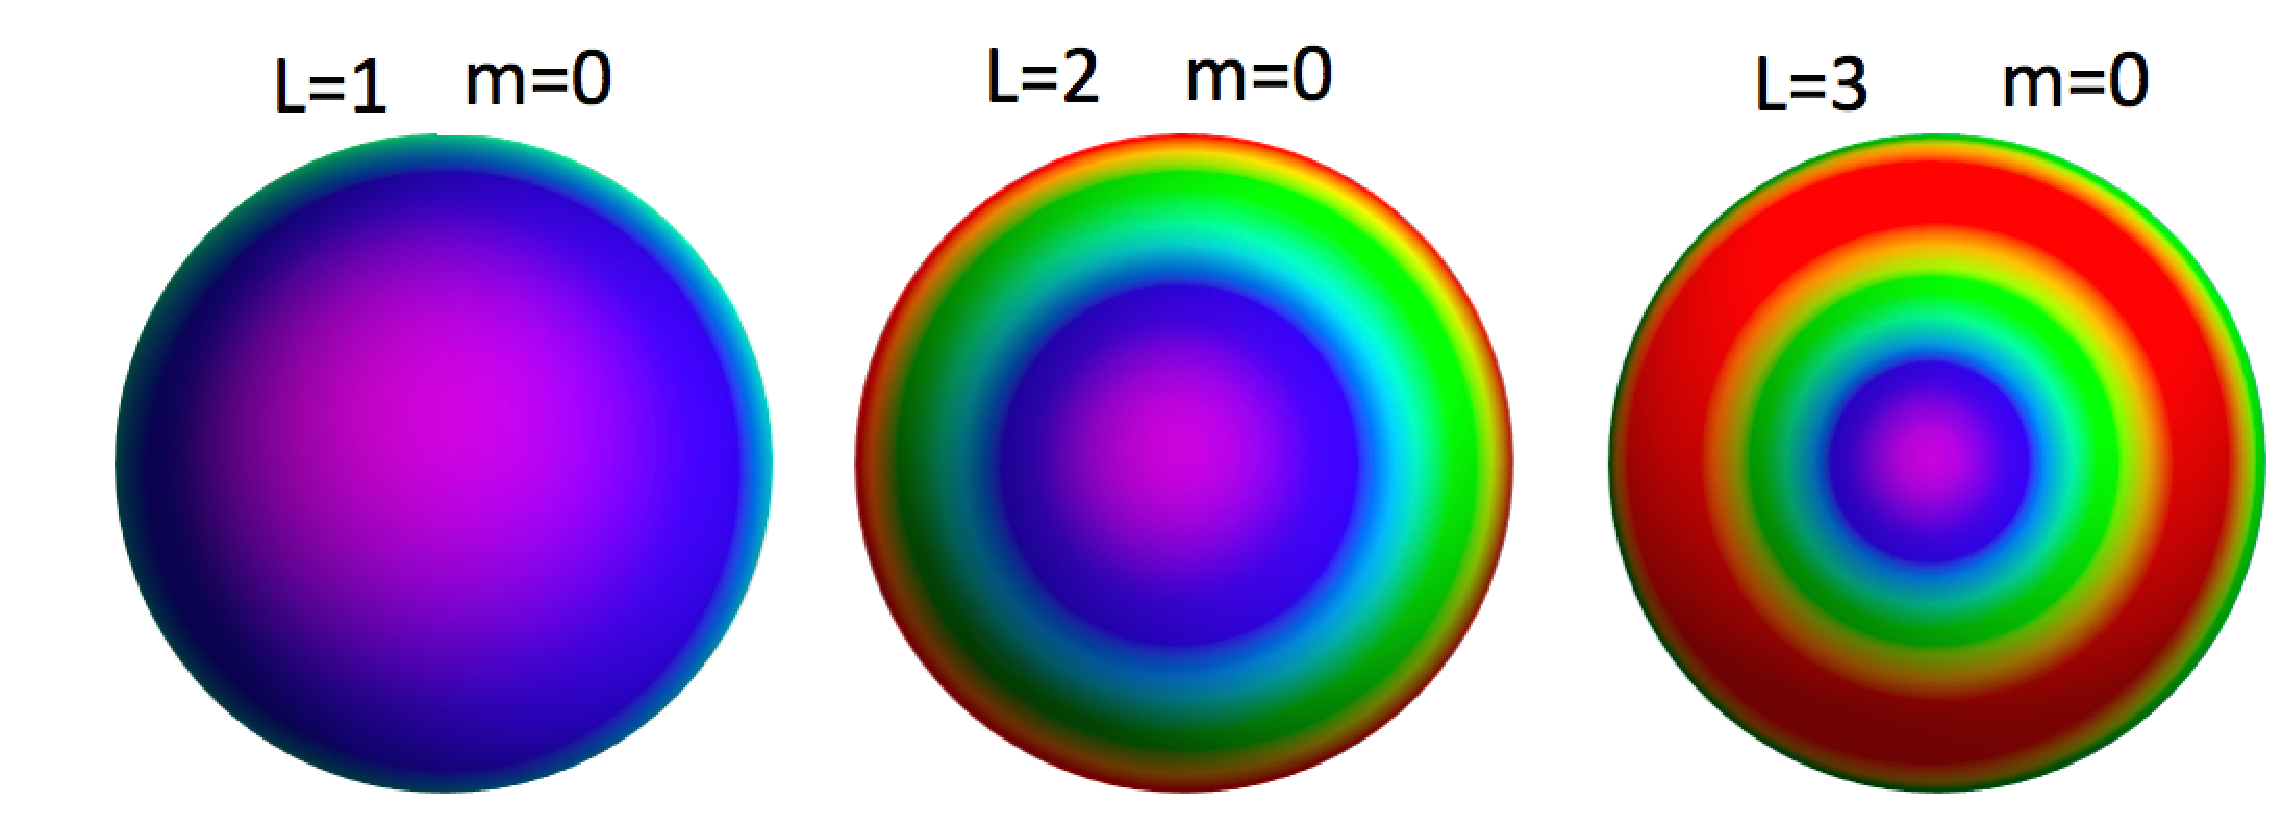
\includegraphics[width=.9\textwidth]{sphazm}
\caption{Plot of spherical harmonics with azimuthal symmetry}
\label{fig:sphazm}
\end{figure}
\subsection{Effect of 4-fold symmetry on Spherical Harmonics Expansion} \label{subsec:fold4}
The behavior of spherical harmonics that has 4-fold symmetry will be thoroughly explained here. The reason 4-fold symmetry is important is that later the object under study is a K-channel protein that satisfies 4-fold symmetry. Studying which expansion vanishes for given particular m quantum number enable one to determine if the object under study has 4-fold symmetry. 

As in the case of azimuthal symmetry, 4-fold symmetry is rotational symmetry with respect to z axis. The spherical harmonics axis can be arbitrary rotated, by setting the center of symmetry as z-axis, selection rule will appear as a result of the symmetry of the object.
\begin{figure}[h]
  \centering
  
\includegraphics[width=.6\textwidth]{4fold2}
\caption{Top view of object with 4-fold symmetry, rotation by $90^{0}$ doesn't change appearance of object }
\label{fig:4fold}
\end{figure}

Figure \ref{fig:4fold} is example of an object which has 4-fold symmetry and the center of symmetry is aligned with the z-axis. Rotation of angle $90^{0}$  or $\pi/2$ doesn't change structure of object. By equating spherical harmonics with the rotated one, one can find the quantum number that satisfy 4-fold symmetry. 
\begin{eqnarray}
Y_{lm}(\theta,\phi)&=&Y_{lm}(\theta,\phi+\frac{\pi}{2}) \\ \nonumber
 Y_{lm}(\theta,\phi)&=&\sqrt{\frac{2l+1}{4 \pi}\frac{(l-m)!}{(l+m)!}} P_{lm}(\cos \theta) e^{im\left(\phi+\pi/2 \right)} \\ \nonumber
\sqrt{\frac{2l+1}{4 \pi}\frac{(l-m)!}{(l+m)!}} P_{lm}(\cos \theta) e^{im\left(\phi \right)} &=& \sqrt{\frac{2l+1}{4 \pi}\frac{(l-m)!}{(l+m)!}} P_{lm}(\cos \theta) e^{im\left(\phi+\pi/2 \right)} \\ \nonumber
e^{im\left(\phi\right)} &=& e^{im\left(\phi+\pi/2 \right)}
\end{eqnarray}
$e^{im\left(\phi\right)} = e^{im\left(\phi+/pi/2 \right)}$ is the requirement to be satisfied if the object has 4-fold symmetry with respect to z-axis. Table \ref{tab:4fold} shows what quantum number persist if the object has 4-fold symmetry. 
\begin{table}[h]
\begin{center}
  \begin{tabular}{ | c | c  |}
    \hline
    m & $e^{im\left(\phi\right)} = e^{im\left(\phi+\pi/2 \right)}$  \\  \hline
    m=0 &\textcolor{red}{1=1} \\  \hline
    m=1 &$\cos( 1 \phi)+ i \sin(1 \phi) \neq \cos(1 (\phi+\pi/2))+ i \sin(1(\phi +\pi/2))$ \\  \hline 
    m=2 &$\cos( 2 \phi)+ i \sin(2 \phi) \neq \cos(2 (\phi+\pi/2))+ i \sin(2(\phi +\pi/2))$ \\  \hline 
    m=3 &$\cos( 3 \phi)+ i \sin(3 \phi) \neq \cos(3 (\phi+\pi/2))+ i \sin(3(\phi +\pi/2))$ \\  \hline 
    m=4 &\textcolor{red}{$\cos( 4 \phi)+ i \sin(4 \phi) = \cos(4 (\phi+\pi/2))+ i \sin(4(\phi +\pi/2))$} \\  \hline 
    m=5 &$\cos( 5 \phi)+ i \sin(5 \phi) \neq \cos(5 (\phi+\pi/2))+ i \sin(5(\phi +\pi/2))$ \\  \hline 
    m=6 &$\cos( 6 \phi)+ i \sin(6 \phi) \neq \cos(6 (\phi+\pi/2))+ i \sin(6(\phi +\pi/2))$ \\  \hline 
    m=7 &$\cos( 7 \phi)+ i \sin(7 \phi) \neq \cos(7 (\phi+\pi/2))+ i \sin(7(\phi +\pi/2))$ \\  \hline 
    m=8 &\textcolor{red}{$\cos( 8 \phi)+ i \sin(8 \phi) = \cos(8 (\phi+\pi/2))+ i \sin(8(\phi +\pi/2))$} \\  \hline 
    \hline
  \end{tabular}
\end{center}
\captionof{table}{Only $m=4n$, where n is integer, satisfy 4-fold symmetry }
\label{tab:4fold}
\end{table}
\begin{figure}[h]
  \centering
  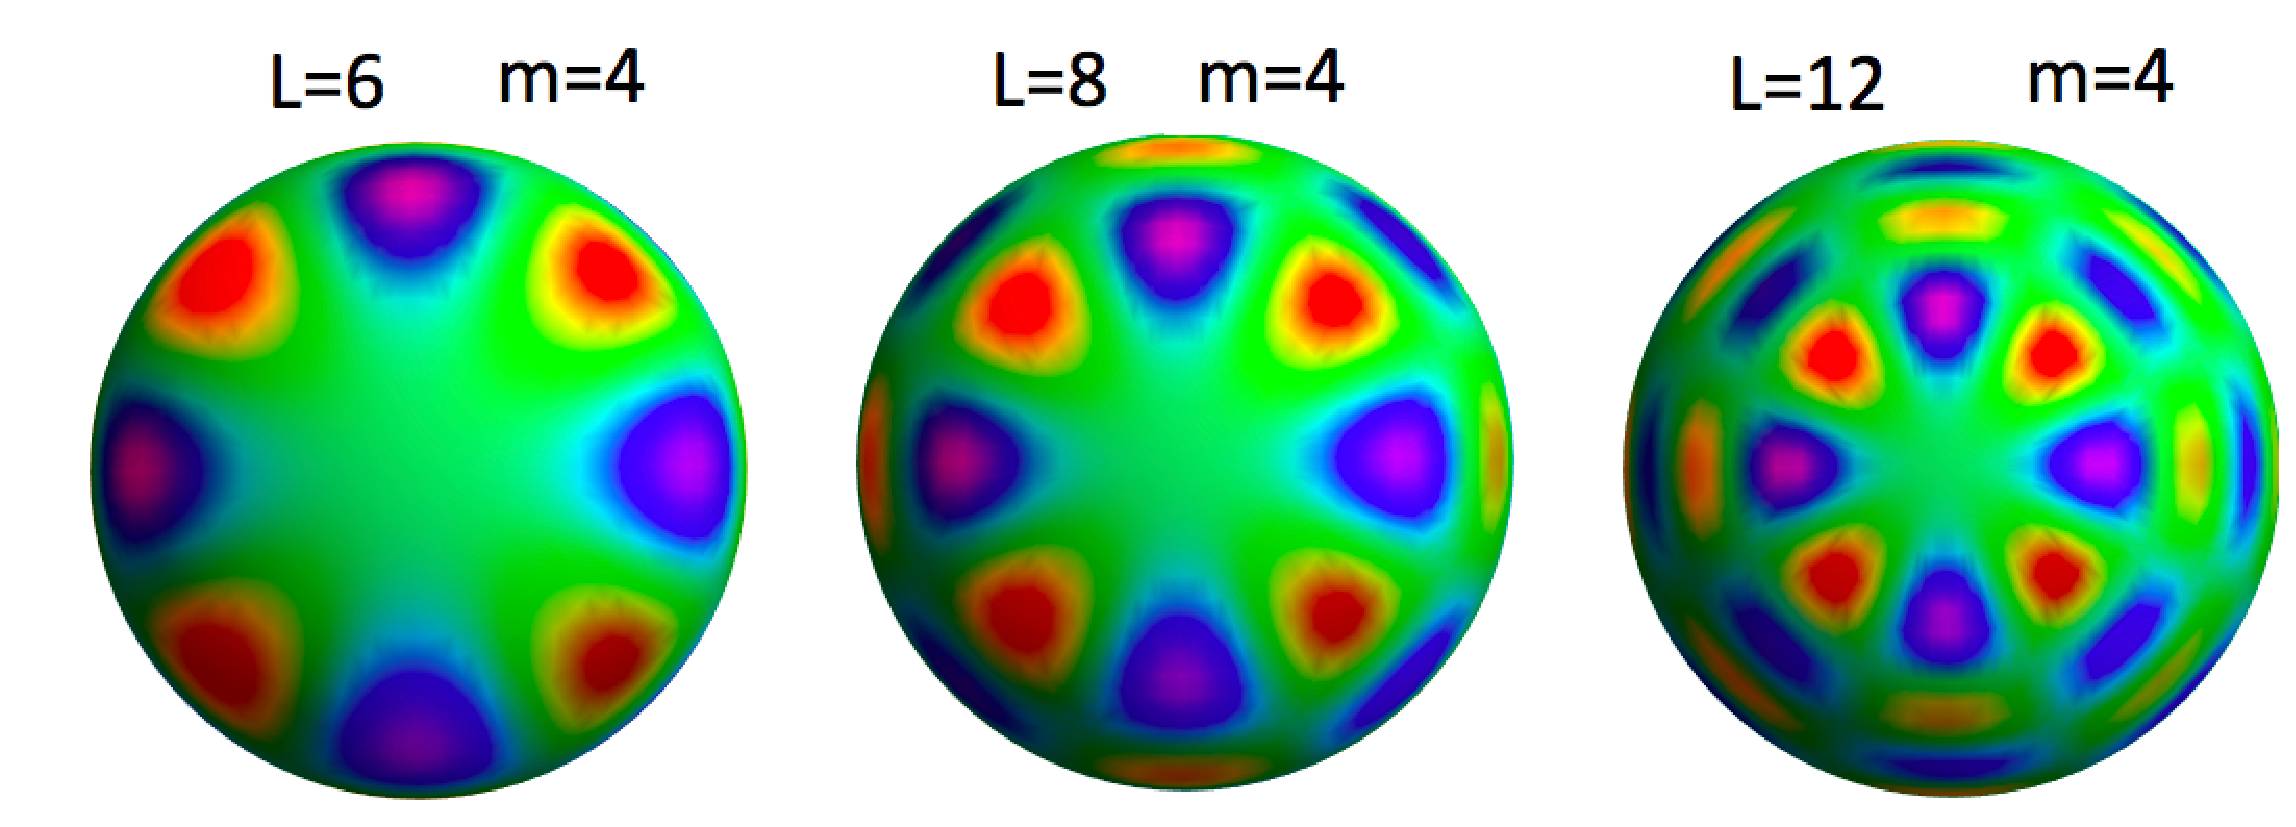
\includegraphics[width=.9\textwidth]{sph4fold}
\caption{Plot of spherical harmonics with 4-fold symmetry}
\label{fig:sph4fold}
\end{figure}
\subsection{Effect of Icosahedral symmetry on Spherical Harmonics Expansion} \label{icosph}
The behavior of spherical harmonics that has icosahedral symmetry will be thoroughly explained here. Previously, the symmetry under study is based on rotation of one axis only and the pattern involve only the $m$ quantum number. More complicated pattern will arise and quantum number in both $m$ and $l$ are necessary. One of symmetry which has more than one rotational axis is icosahedral symmetry. Studying which expansion vanishes for given particular m quantum number enable one to determine if the object under study has 4-fold symmetry.

Different than azimuthal and 4-fold symmetry, icosahedral symmetry has 3 rotational axes. They are 5-fold, 3-fold and 2-fold axes. The z-axis can be chosen arbitrary, by setting the center of symmetry as the 5-fold axis unique selection rule will appear as a result of the symmetry of the object. Based on icosahedral selection rule\cite{norahcohan}, $I_{lm}$ is nonzero when $l$ satisfy. 
\begin{eqnarray}
l=6p+10q \\
\text{where p and q in integer} \nonumber
\end{eqnarray}
and $m$ quantum numbers are
\begin{eqnarray}
m=...,-10,-5,0,5,10,...
\end{eqnarray}
when of 5-fold axis is taken as the z-axis. 
\begin{figure}[h]
  \centering
  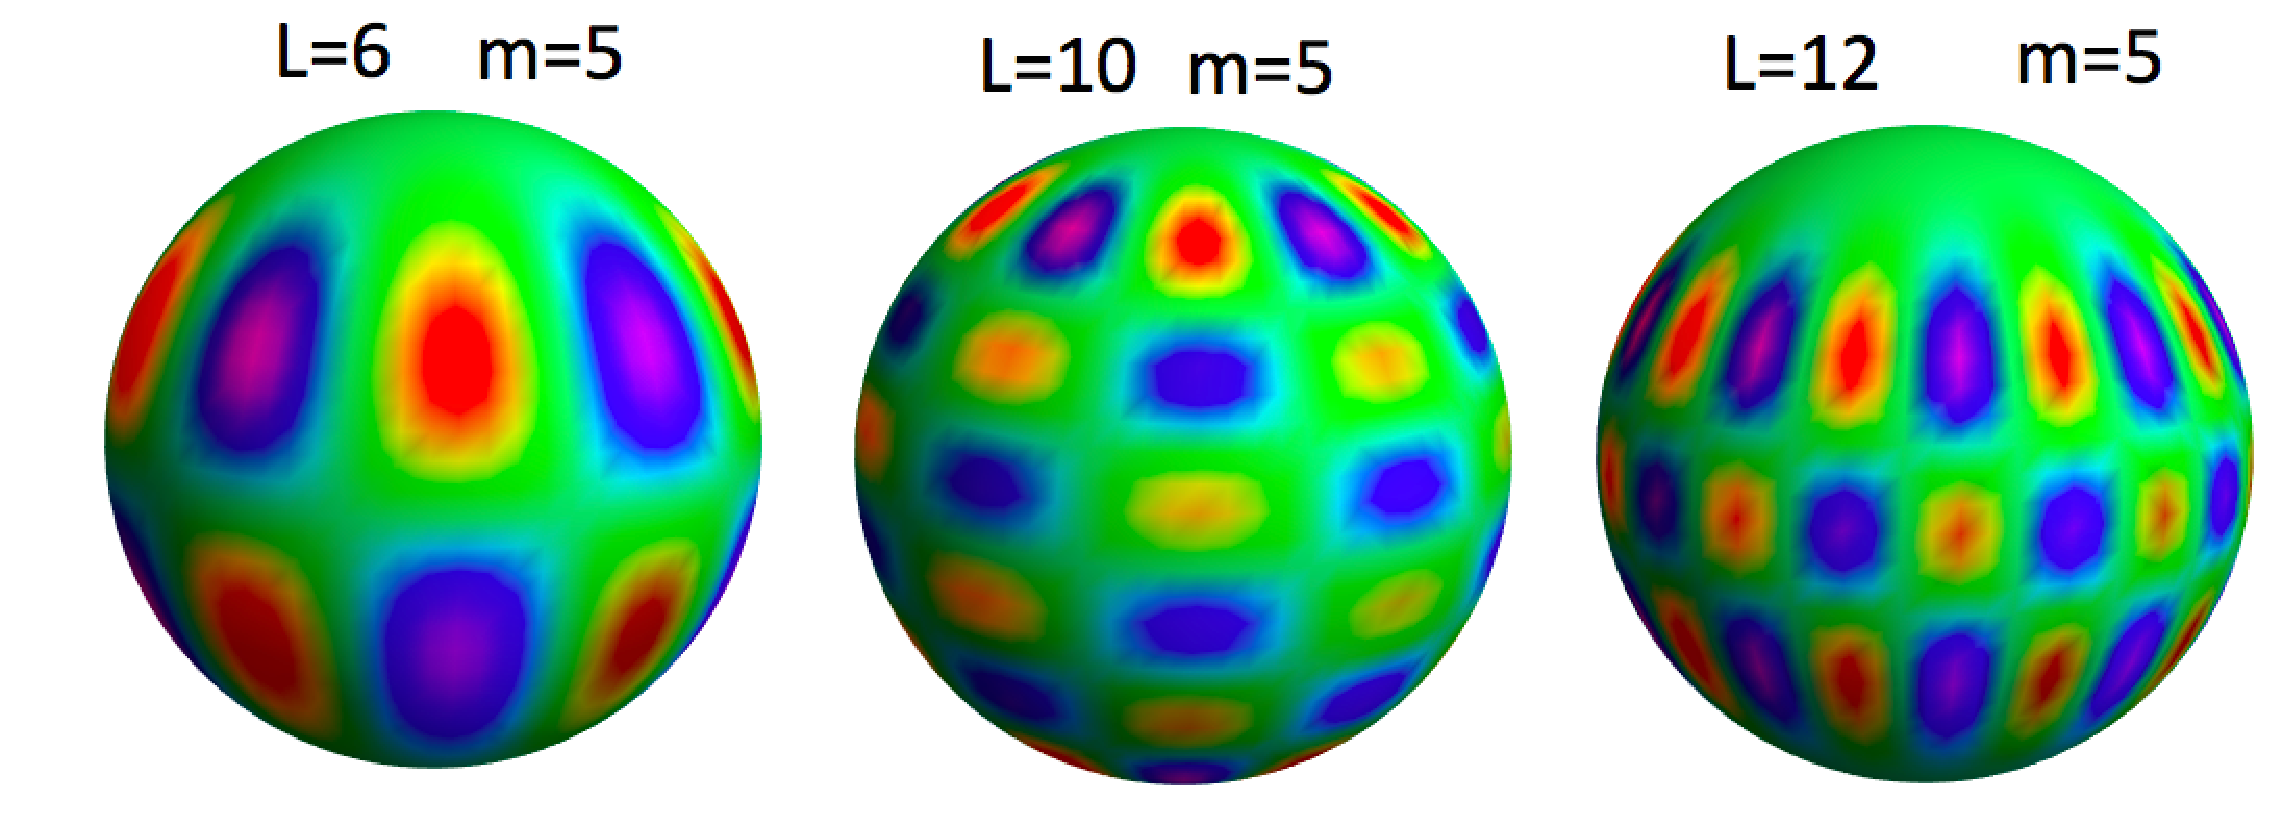
\includegraphics[width=.9\textwidth]{spico}
\caption{Plot of spherical harmonics with icosahedral symmetry}
\label{fig:icosymsph}
\end{figure}
A function can be constructed from a linear combination of spherical harmonics. In order to the function to satisfy icosahedral symmetry then only spherical harmonics which satisfies the selection rule are taken into the linear combination. In equation \ref{eq:icoharmonics}, $J_{l}(\theta,\phi)$ is an icosahedral harmonic which consist of a linear combination of spherical harmonics. By summing over all $m$, icosahedral harmonics only depend on $l$ quantum number.  

Factor $a_{lm}$ cannot be arbitrary because equation \ref{eq:icoharmonics} must satisfy icosahaderal symmetry\cite{harisonjack}. Table \ref{tab:spico} shows values of $a_{lm}$ for different combination of $l$ and $m$. Icosahedral harmonics are defined as linear combination of spherical harmonics which satisfy icosahedral symmetry:  
\begin{table}[h]
\begin{center}
  \begin{tabular}{ | c | c  | c | c | c | c |}
    \hline
    l\ m & 0 & 5 & 10 & 15 & 20  \\  \hline
    0 & 1.0 & & & &  \\  \hline
    6 & 0.531085 & 0.847318 & & & \\  \hline 
    10 &0.265539 &-0.846143 &0.462094 & & \\  \hline 
    12 &0.454749 &0.469992 &0.75613 & & \\  \hline 
    16 &0.334300 &-0.493693 &-0.634406 &0.491975 &\\  \hline 
    18 &0.399497 &0.450611 &0.360958 &0.712083 &\\  \hline 
    20 &0.077539 &-0.460748 &0.747888 &-0.231074 &0.411056\\  \hline 
    \hline
  \end{tabular}
\end{center}
\captionof{table}{Coefficient of spherical harmonics to convert into icosahedral harmonics \cite{saldinvirus} }
\label{tab:spico}
\end{table}
\begin{eqnarray}
J_{l}(\theta,\phi)=\sum_{m} a_{lm} Y_{lm}(\theta,\phi)
\label{eq:icoharmonics}
\end{eqnarray}
From table \ref{tab:spico}, $I_{lm}$ is nonzero if $m$ is a multiple 5. By looking at equation \ref{eq:icoharmonics}, for a particular $l$, $I_{lm}$ is not independent if the object has icosahedral symmetry. The spherical harmonics expansion of an icosahedral object only depends on values of $l$, given the $l$ the values of $m$ are determined by symmetry and are tabulated. In other words, for icosahedral object there is one independent parameter for each $I_{lm}$.


% CHAPTER 2 Section Symmetry on Angular Correlation
\section{Symmetry on Angular Correlation}
\subsection{Rotation of Data Points} \label{sec:PCA}
This section explains relation of rotation matrices and data points. It will be shown that redundancy or lowest number of independent parameter can be found by applying particular rotation matrix on data points.

Orthogonal transformation is a linear transformation that preserves the dot product of vectors. The length or radius of the vectors are not changed by applying an orthogonal transformation. Even more, the angle between two vectors are preserved. Applying orthogonal transformation on coordinate axes will result in rotation, reflection, or inversion of axes. Mathematically, an orthogonal transformation is represented as a rotation matrix. Basic theory about orthogonal transformations and rotation matrices is described in this section.   

\begin{figure}[h]
\begin{subfigure}{.5\textwidth}
  \centering
  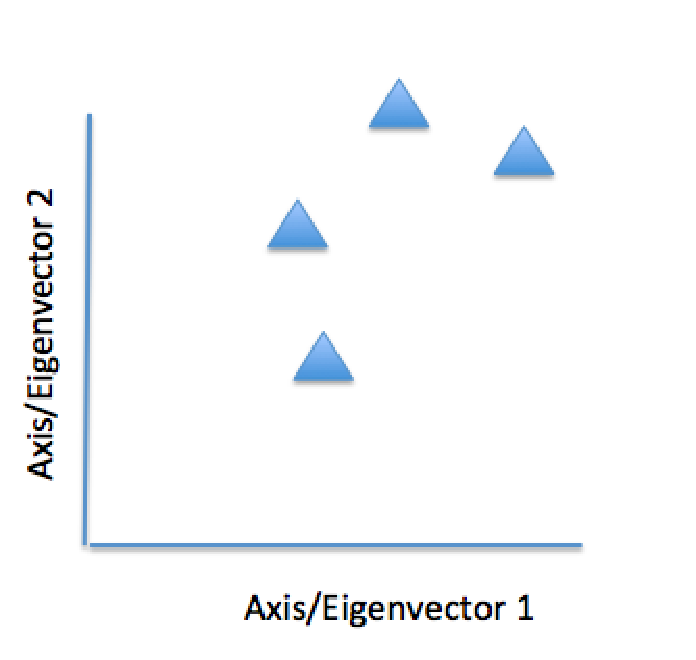
\includegraphics[width=.6\textwidth]{pointfree}
  \caption{Original axis}
\end{subfigure}
\begin{subfigure}{.5\textwidth}
  \centering
  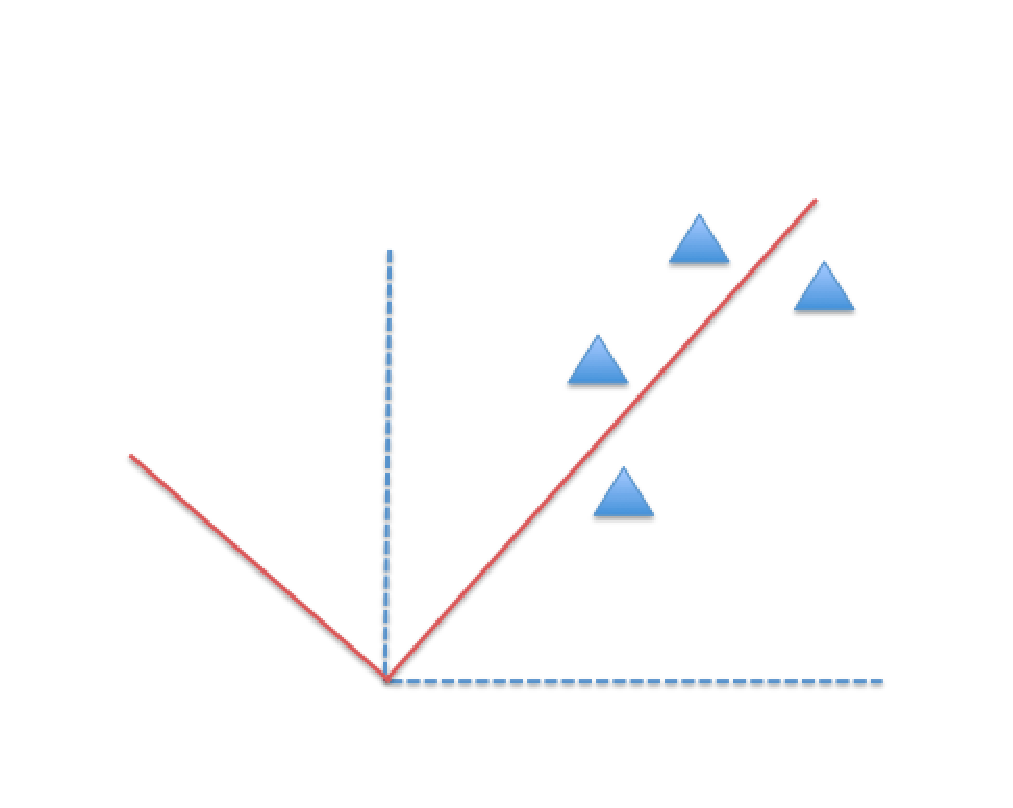
\includegraphics[width=.8\textwidth]{rotatedpoint}
  \caption{Rotated axis}
\end{subfigure}
\caption{Any point can be described in transformed axis}
\label{fig:rotatedaxis}
\end{figure}

Figure \ref{fig:rotatedaxis} illustrates that any point can be described in terms of any axes. As long as the relation of the new to the old axes is caused by an orthogonal transformation, the effect on data points is only rotation,  preserving radius or length of the data points. Throughout all rotation, there will be always an axis or direction in which one particular axis will have a smallest component as displayed in figure \ref{fig:axissmallercomponent},  By knowing that axis, it can be used to reduce the dimension of the data without losing essential information because axis with the smallest component has the least information.    



\begin{figure}[h]
  \centering
  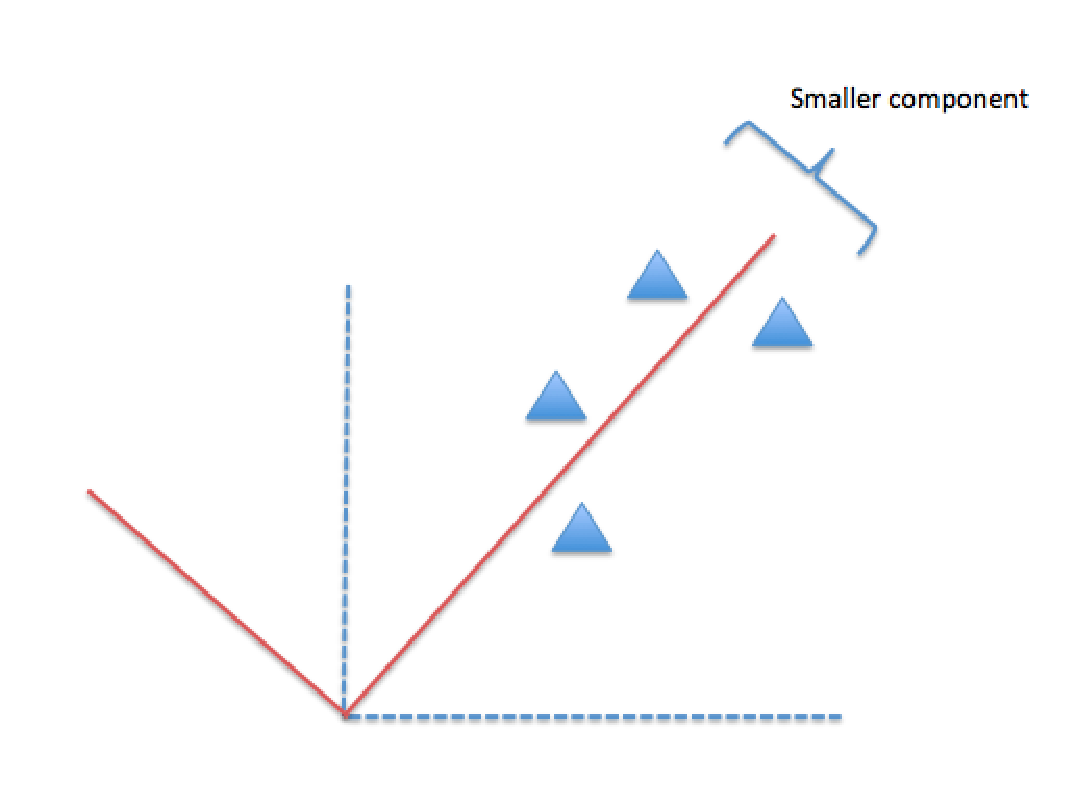
\includegraphics[width=.8\textwidth]{rotatedpointsmaller}
\caption{Red is axis in which has maximum variance in one direction and minimum component in another one}
\label{fig:axissmallercomponent}
\end{figure}

\begin{figure}[h]
  \centering
  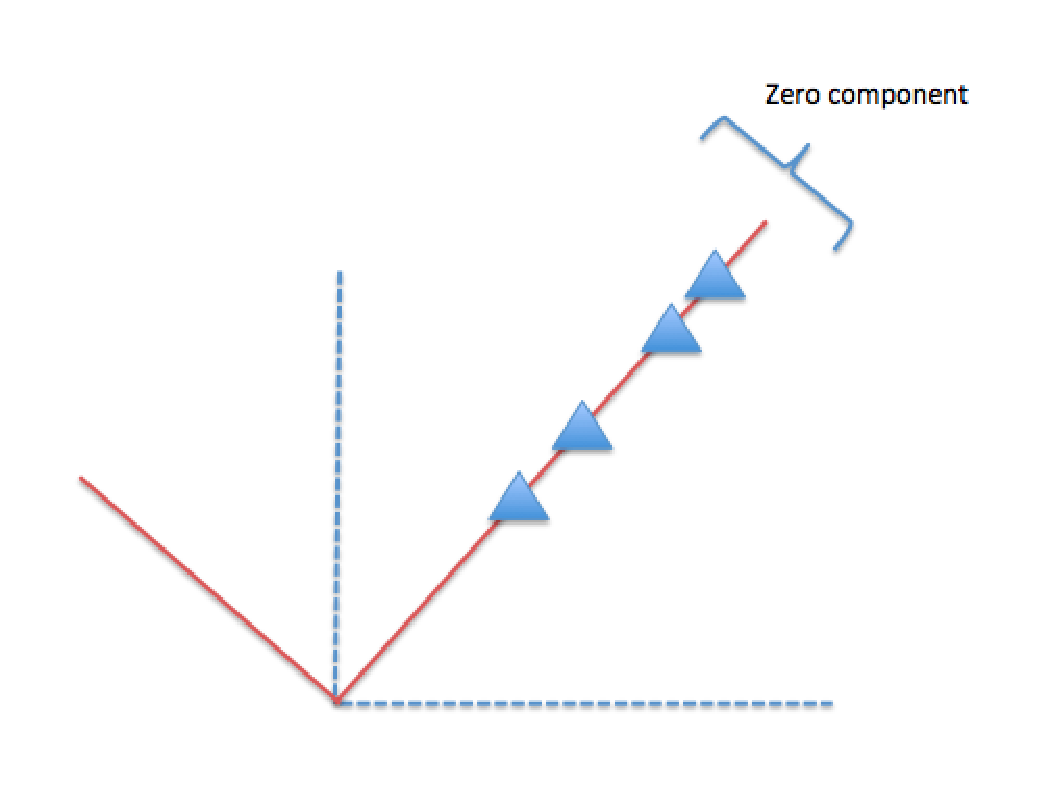
\includegraphics[width=.8\textwidth]{rotatedpointzero}
\caption{In red axis, data can be specified with one parameter only}
\label{fig:axisoneparameter}
\end{figure}
A rotation matrix can be used to indicate whether there is redundant information in data set. A redundancy means there is a different way to represent data with a lower number of independent parameters. Illustrated in figure \ref{fig:axisoneparameter}, the data points are represented by two different ways, using blue axes the data are specified using two parameters whereas using the red axis the data are specified with one parameter. If the data contain redundant information, then the number of independent parameters can be reduced by rotating the axes. Figure \ref{fig:axisoneparameter} shows that redundancy in 2D occurs due to the data lying in the same line. Generalizing into higher dimension, the redundancy occur  when the data lie in either a line, a plane, or a hyperplane. 

Essential property to find the lowest number of independent parameter is knowing that the dot product between the  data set is enough to reveal the redundancies.  From figure \ref{fig:axisoneparameter}, all data point have the same angle from each other. Since the angle is obtainable from the dot product, by constructing a matrix of dot products, a pattern appear whether there is a redundancy inside data sets. The redundancy in 2D case is very simple; if the angle is the same for the all data set, then there is redundancy. To reveal the redundancy in higher order, a different sophisticated method is needed, because a common pattern in dot product is not easily observable. 

One of the method to reveal redundancy of the data in higher dimension is the principal component analysis. The next section will explain the principal component analysis and how it can be used to determine symmetry of particles only from correlation data.  

\subsection{Principal Component  Analysis }
Principal component analysis (PCA) is an established method to reduce the dimension of a set of vectors. PCA uses orthogonal transformation to convert a set of vectors into a set of new vectors. The determination of the orthogonal transformation is defined in such a way that one axis will have the largest variance and another axis will have the smallest component. In addition to that, PCA can be used to find the lowest number of independent parameters in a data set, which is the purpose of this section. 

Another important point is that the rotation of an axis can be used to find the lowest number of independent parameters in the data set. A set of vectors in any arbitrary independent axis can be described as
\begin{eqnarray}
\vec{V_{1}}=
\begin{bmatrix}
\upsilon_{11}&\upsilon_{12} & \ldots & \upsilon_{1m}
\end{bmatrix}\\ \nonumber
\vec{V_{2}}=
\begin{bmatrix}
\upsilon_{21}&\upsilon_{22} & \ldots & \upsilon_{2m}
\end{bmatrix}\\ \nonumber
\vec{V_{3}}=
\begin{bmatrix}
\upsilon_{31}&\upsilon_{32} & \ldots & \upsilon_{3m}
\end{bmatrix}\\ \nonumber
\vec{V_{n}}=
\begin{bmatrix}
\upsilon_{n1}&\upsilon_{n2} & \ldots & \upsilon_{nm}
\end{bmatrix}\\ \nonumber
.
\end{eqnarray}
To represent this set of vectors as a set of new data, a matrix can be formed by arranging each row as new independent vectors and each column as an independent components. The matrix is  
\begin{eqnarray}
\mathbf{V}=
\begin{bmatrix}
\upsilon_{11}&\upsilon_{12} & \ldots & \upsilon_{1m} \\
\upsilon_{21}&\upsilon_{22} & \ldots & \upsilon_{2m} \\
\upsilon_{31}&\upsilon_{32} & \ldots & \upsilon_{3m} \\
\vdots & \vdots \\
\upsilon_{n1}&\upsilon_{n2} & \ldots & \upsilon_{nm} 
\end{bmatrix}.
\end{eqnarray} 
From that new definition, a new quantity called covariance matrix is defined as
\begin{eqnarray}
\mathbf{C}=\mathbf{V^{t}}\mathbf{V}.
\end{eqnarray} 

Based on PCA, the first eigenvector of the covariance matrix is the direction of the maximum variance or the minimum residual component. In addition to that, finding the lowest independent parameters to describe the system can be found from counting the nonzero eigenvalues of the covariance matrix. In addition to that, calculating eigenvectors and eigenvalues can be done by using singular value decomposition (SVD). Mathematically, the SVD is 

\begin{eqnarray}
[u \, s \, v ]=\mbox{SVD}(\mathbf{V^{t}}\mathbf{V})
\end{eqnarray} 
where $u$ is a matrix composed of independent eigenvectors and $s$ is a matrix consist of eigenvalues of covariance matrix. 

Neither $\mathbf{V^{t}}\mathbf{V}$ nor $\mathbf{V}$ are available from the angular correlation data. Only the matrix of dot product is available. It will be shown below that matrix of dot product will have eigenvalues equal to the eigenvalues of covariance matrix. 

The matrix of the dot product is defined as
\begin{eqnarray}
\mathbf{M_{d}} &=& 
\begin{bmatrix}
\vec{V_{1}}\cdot\vec{V_{1}} &\vec{V_{1}}\cdot\vec{V_{2}} & \ldots & \vec{V_{1}}\cdot\vec{V_{m}} \\
\vec{V_{2}}\cdot\vec{V_{1}} &\vec{V_{2}}\cdot\vec{V_{2}} & \ldots & \vec{V_{2}}\cdot\vec{V_{m}} \\
\vec{V_{3}}\cdot\vec{V_{1}} &\vec{V_{3}}\cdot\vec{V_{2}} & \ldots & \vec{V_{3}}\cdot\vec{V_{m}} \\
\vdots & \vdots \\
\vec{V_{n}}\cdot\vec{V_{1}} &\vec{V_{n}}\cdot\vec{V_{2}} & \ldots & \vec{V_{n}}\cdot\vec{V_{m}} \\
\end{bmatrix}
\\
&=& \vec{V} \vec{V^{t}}.
\end{eqnarray}
Having defined the matrix of the dot product, its eigenvalue can be found from the covarianve matrix or covariance matrix's eigenvalue can be found from the matrix of the dot product. The proof is shown below: 
\begin{eqnarray}
\mathbf{M_{d}} \, \nu &=& \lambda \, \nu \\ \nonumber
\vec{V} \, \vec{V^{t}} \, \nu &=& \lambda \, \nu \\ \nonumber
%\mbox{left multiplication with } \vec{V^{t}} \mbox{yield}  \\
\vec{V^{t}} \, \vec{V} \, \vec{V^{t}} \, \nu &=& \lambda \, \vec{V^{t}}\, \nu \\ \nonumber
\vec{V^{t}} \, \vec{V} \, \mu &=& \lambda \, \mu 
\label{eq:matrixofdotproduct}
\end{eqnarray}

In conclusion, $\vec{V} \, \vec{V^{t}}$ and $\vec{V^{t}} \, \vec{V}$ have equal eigenvalues but different eigenvectors. The eigenvalue that give the lowest independent component is the eigenvalue of the covariance matrix. Hence, the eigenvalue of the covariance matrix can be easily be calculated by finding the eigenvalue of matrix of dot product. 

\subsection{Matrix Correlation}
As described in section \ref{sec:angcor}, the final expression obtained from the correlation data is
\begin{eqnarray}
B_{l}(q,q')=\sum_{m} I_{lm}(q) I_{lm}(q')^{*}. 
\end{eqnarray}
It is important to note that \Blq is a form of dot product depending of how one constructs vectors from $I_{lm}(q)$. Since every $I_{lm}(q)$ comes from spherical harmonics decomposition, every element is independent. A set of new vectors can be constructed where the value $m$'s correspond to the components and $q$'s correspond to the vectors for all $l$'s. As an example, the vectors constructed from this definition are
\begin{eqnarray}
I_{l}(q_1)=
\begin{bmatrix}
I_{l(-l)}(q_1)&I_{l(-l+1)}(q_1) & \ldots &I_{l(l)}(q_1)
\end{bmatrix}\\ \nonumber
I_{l}(q_2)=
\begin{bmatrix}
I_{l(-l)}(q_2)&I_{l(-l+1)}(q_2) & \ldots &I_{l(l)}(q_2)
\end{bmatrix}\\ \nonumber
I_{l}(q_3)=
\begin{bmatrix}
I_{l(-l)}(q_3)&I_{l(-l+1)}(q_3) & \ldots &I_{l(l)}(q_3)
\end{bmatrix}\\ \nonumber
I_{l}(q_n)=
\begin{bmatrix}
I_{l(-l)}(q_n)&I_{l(-l+1)}(q_n) & \ldots &I_{l(l)}(q_n)
\end{bmatrix}.\\ \nonumber
\end{eqnarray}
The expression $\sum_{m} I_{lm}(q) I_{lm}(q')^{*}$ is equivalent to $ \langle I_{l}(q) , I_{l}(q') \rangle$ that is the dot product of $I_{l}(q)$. Now with that definition, \Blq is a dot product of vectors $I_{lm}(q)$. 

After confirming that \Blq is the dot product of the vector \Ilm, a new matrix must be constructed in order to be used in PCA. There are infinite possible ways to construct a matrix from a set of vectors. In order to be used in PCA, the matrix of dot products is constructed by arranging all possible dot products of different vectors or $q$ points. Below is how matrix is constructed
\begin{eqnarray}
\mathbf{B_{qq'}^{l}} &=& 
\begin{bmatrix}
\langle I_{l}(q_1), I_{l}(q_1)\rangle & \langle I_{l}(q_1),I_{l}(q_2) \rangle & \ldots & \langle I_{l}(q_1),I_{l}(q_m) \rangle \\
& & \\
\langle I_{l}(q_2), I_{l}(q_1)\rangle & \langle I_{l}(q_2),I_{l}(q_2) \rangle & \ldots & \langle I_{l}(q_2),I_{l}(q_m) \rangle \\
& &\\
\langle I_{l}(q_3), I_{l}(q_1)\rangle & \langle I_{l}(q_3),I_{l}(q_2) \rangle & \ldots & \langle I_{l}(q_3),I_{l}(q_m) \rangle \\
\vdots & \vdots & \vdots \\
\langle I_{l}(q_n), I_{l}(q_1)\rangle & \langle I_{l}(q_n),I_{l}(q_2) \rangle & \ldots & \langle I_{l}(q_n),I_{l}(q_m) \rangle \\
\end{bmatrix}
\\
&=&
\begin{bmatrix}
B_{l}(q_1,q_1) &B_{l}(q_1,q_2)& \ldots& B_{l}(q_1,q_m) \\
& & \\
B_{l}(q_2,q_1) &B_{l}(q_2,q_2)& \ldots& B_{l}(q_2,q_m) \\
& &\\
B_{l}(q_3,q_1) &B_{l}(q_3,q_2)& \ldots& B_{l}(q_3,q_m) \\
\vdots & \vdots & \vdots \\
B_{l}(q_n,q_1) &B_{l}(q_n,q_2)& \ldots& B_{l}(q_n,q_m) \\
\end{bmatrix}
\end{eqnarray}

All elements of matrix $\mathbf{B_{qq'}}$ are obtainable from experiment according to eq \ref{eq:theB}. The matrix satisfies requirement to be a matrix of dot product as given in eq. \ref{eq:matrixofdotproduct}. The singular values of the matrix contain the information about the redundancy of the data. By counting how many nonzero singular value, those number can be used to describe the redundancy in vector $I_{lm}(q)$. 

The number of significant nonzero singular values represent total parameter to describe the data. Only nonzero singular value contribute to the independent parameters. The nonsignificant or zero singular values denote the number of redundant parameters. By comparing how many significant or nonzero, nonsignificant or zero, and total singular values, those information later is essential to predict the symmetry of the particle. 
%\end{document}


%CHAPTER 3 Section Pattern on Symmetry
\chapter{Result}
\section{Pattern on Symmetry}\label{sec:pattsymm}
\subsection{Azimuthal Pattern}
Given in section \ref{sec:PCA}, there will be a particular pattern of nonzero singular values depending on the symmetry of the object. In the section \ref{subsec:azimsym}, it is explained that the azimuthal spherical harmonics components can be described by only one $m$ value for each $l$ or in other words only $m=0$ is nonzero. If the object has azimuthal symmetry then the matrix \Blq will only have one non zero significant singular value. 
\begin{figure}[ht]
  \centering
  
\includegraphics[width=.4\textwidth]{ellipsoid}
\caption{Model which has azimuthal symmetry}
\label{fig:ellipsoid}
\end{figure}

Figure \ref{fig:ellipsoid} is a model that is used to calculate \Blq. The model is ellipsoid which satisfy pure azimuthal symmetry, therefore \Blq inherently contain azimuthal symmetry. By taking SVD of the \Blq, the redundancy will be revealed and can be used to deduce the symmetry of object.
 \begin{figure}[ht]
  \centering
  \includegraphics[width=.8\textwidth]{azimsvd}
\caption{Total number of nonzero singular values vs angular momentum}
\label{fig:azimsvd}
\end{figure}
\begin{figure}[ht]
  \centering
  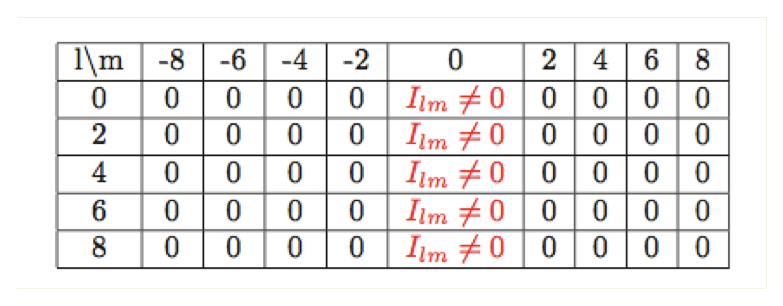
\includegraphics[width=.6\textwidth]{tableIlmazim}
\caption{Table of nonzero $I_{lm}$ for azimuthal symmetry}
\label{fig:azimtable}
\end{figure}

The graph on figure \ref{fig:azimsvd} shows the behavior of the singular value of the object which has azimuthal symmetry. It shows that only one nonzero singular value for each $l$, therefore it matchs the behavior of $I_{lm}$ which only $m=0$ is not vanish. Having said that, SVD of \Blq can be used to predict if the object satisfy azimuthal symmetry. 

\subsection{4-fold Pattern}
The example given here is for the object that has 4-fold symmetry. However in general it can be extended to any n-fold symmetry without losing of uniqueness. In the section \ref{subsec:fold4}, it is explained that if a 4-fold symmetry exist then the component of spherical harmonics, which the $l$'s are a multiple value of 4, will be nonzero. As consequence of that, the number of nonzero singular values of the matrix \Blq has pattern that match with the total number of nonzero components in spherical harmonics expansion.  

\begin{figure}[ht]
  \centering
  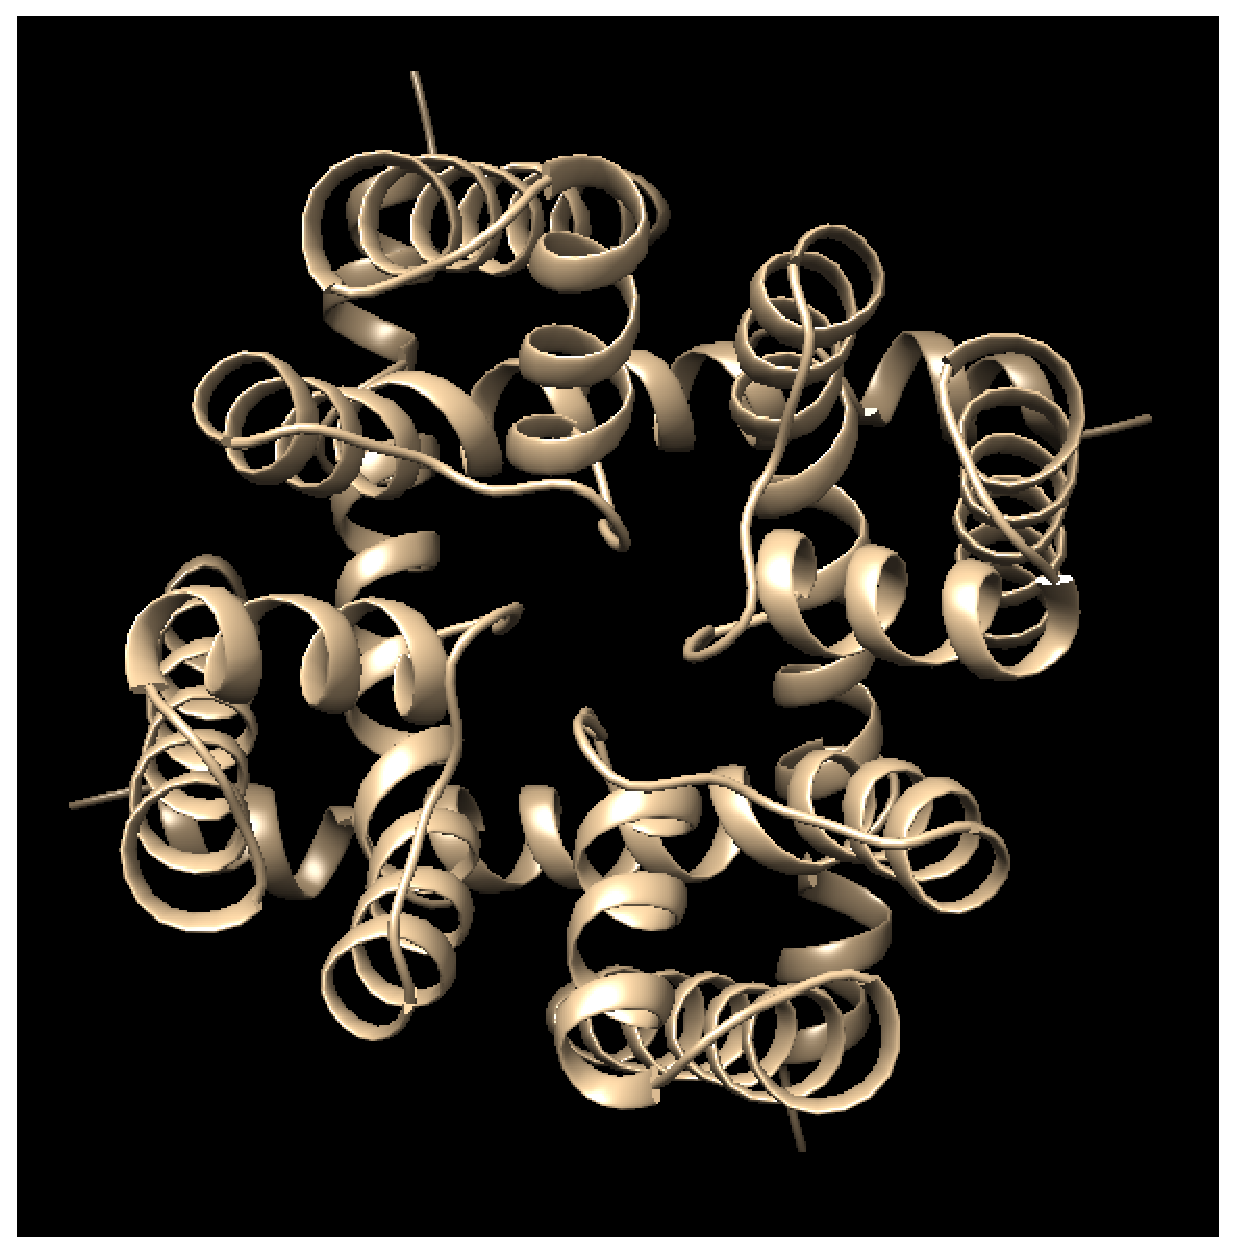
\includegraphics[width=.6\textwidth]{KC4fold}
\caption{K-channel protein has 4-fold symmetry}
\label{fig:KC4fold}
\end{figure}

The figure \ref{fig:KC4fold} shows 4-fold symmetric model that is used to calculate \Blq. 
Because the model has 4-fold symmetry, the \Blq inherently contain information about the 4-fold symmetry. 
By taking SVD of the \Blq, the redundancy will be revealed and can be used to deduce the symmetry of object. From figure \ref{fig:4foldsvd} and table \ref{fig:4foldtable}, there is a matching pattern. By comparing them, for $l=2$ there is one nonzero singular value and there is only one nonzero $I_{lm}$ that is when $m=0$. 
Another example is for $l=6$, there are 4 singular value from figure  \ref{fig:4foldsvd} and from table \ref{fig:4foldtable} there are 3 nonzero $I_{lm}$ that is when $m=-4,0,4$. If unknown structure give the same behavior as in graph \ref{fig:4foldsvd} then one can conclude it has 4-fold symmetry. 
\begin{figure}[h]
  \centering
  \includegraphics[width=.8\textwidth]{svdKC}
\caption{Total number of nonzero singular values vs angular momentum}
\label{fig:4foldsvd}
\end{figure}
\begin{figure}[ht]
  \centering
  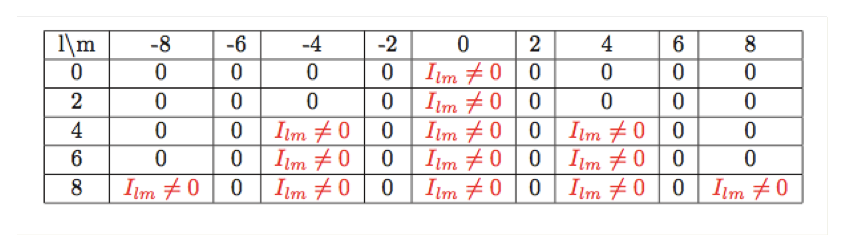
\includegraphics[width=.6\textwidth]{tableIlm4fold}
\caption{Table of nonzero $I_{lm}$ for 4-fold symmetry}
\label{fig:4foldtable}
\end{figure}

\subsection{Icosahedral Pattern}
One of the important symmetry to be demonstrated in this section is icosahedral symmetry. Previous section explains that there is only one singular value of \Blq if the object has icosahedral symmetry.
 In addition to that, there is a selection rule of $l$'s for icosahedral harmonics. In order to predict the icosahedral symmetry both the selection rule and the singular value has to be satisfied. 
\begin{figure}[h!]
  \centering
  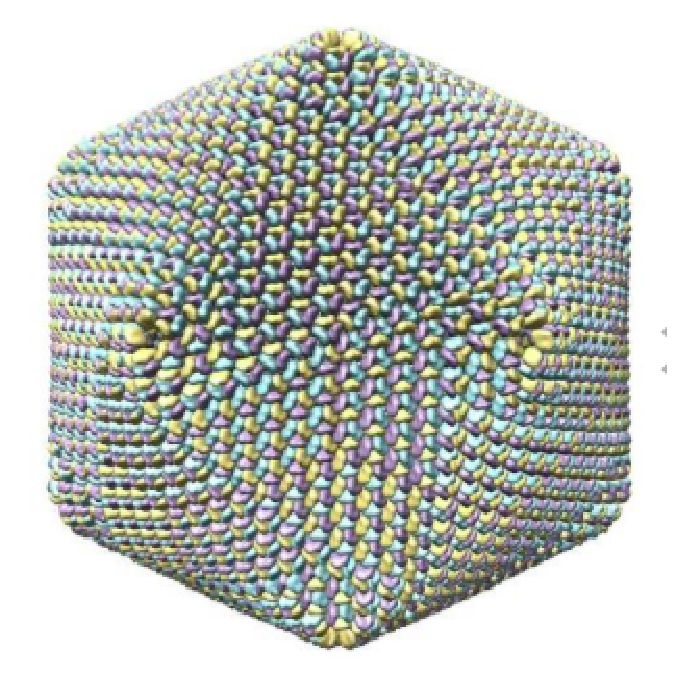
\includegraphics[width=.5\textwidth]{cor}
\caption{PBCV from pdb(1m4x) is used as model that has icosahedral symmetry \cite{pdb1m4x}}
\label{fig:icopbcv}
\end{figure}

The figure \ref{fig:icopbcv} is model that is used to calculate \Blq. The model is a virus that satisfy pure icosahedral symmetry. Thus, \Blq inherently contain the icosahedral symmetry. By taking SVD of \Blq, the redundancy will be revealed and can be used to deduce the symmetry of the object.
\begin{figure}[h!]
  \centering
  \includegraphics[width=.8\textwidth]{svdBcor}
\caption{Total number of nonzero singular values vs angular momentum}
\label{fig:svdico}
\end{figure}

The figure \ref{fig:svdico} is a graph calculated from svd of \Blq. It is obviously seen that it follows icosahedral selection rule and at the same time has one singular value for each $l$. If unknown structure give behavior as in graph \ref{fig:svdico} then one can conclude it has icosahedral symmetry.   
\subsection{Asymmetric Pattern}
In this section distinguishing  asymmetric property is demonstrated. Previous section explains that there will be $2l+1$ singular value if the object under study has asymmetric property. The number of singular values is equal to total component in spherical harmonics expansion. 
\begin{figure}[h!]
  \centering
  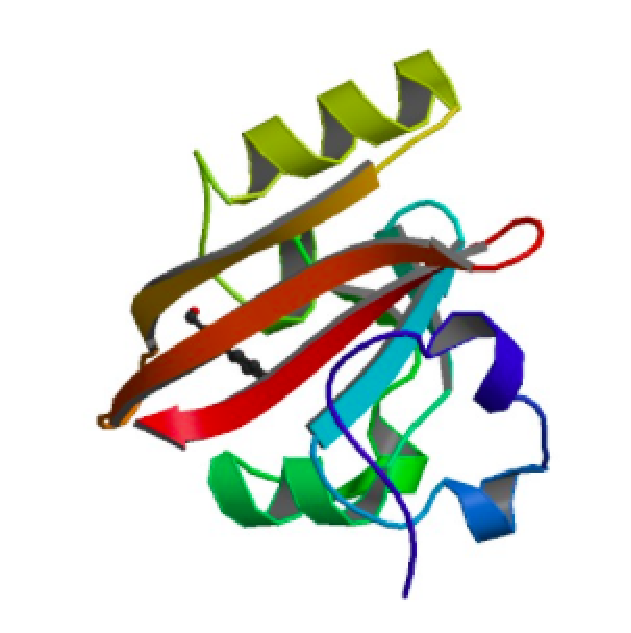
\includegraphics[width=.5\textwidth]{pyp}
\caption{Photoactive yellow protein from pdb(2phy) is used as model}
\label{fig:pyp}
\end{figure}

The figure \ref{fig:pyp} is a model that is used to calculate \Blq. The model is pyp protein, which doesn't have symmetry at all, therefore \Blq inherently contain asymmetric property. From figure \ref{fig:svdPYP}, for every $l$'s there are $2L+1$ singular values. As already mentioned before, $2l+1$ singular values represent asymmetric pattern. If an unknown structure give a behavior as in graph \ref{fig:svdPYP} then one can conclude that it has asymmetry property.   
\begin{figure}[h!]
  \centering
  \includegraphics[width=.8\textwidth]{svdBaPYP}
\caption{Total number of nonzero singular values vs angular momentum}
\label{fig:svdPYP}
\end{figure}

This asymmetric pattern can be used to inspect whether \Blq is a form of a dot product. Because no shape can be more asymmetrical than asymmetric shape, no shape can have more number of singular values than an asymmetric shape. In other words, $2l+1$ is the highest number of singular values and all shapes should have number of singular values less than or equal $2l+1$. If an SVD on the \Blq has more singular values than $2l+1$ then the \Blq is not a form of dot product or convergence is not reached.  


\subsection{Inversion Symmetry}
This section describes one of the limits of the methods (PCA and selection rule) by giving an analysis of applying inversion symmetry. Because the available data from the experiment is a collection of diffraction patterns, all analyses initially have to be done in reciprocal space. It applies also to the determination of symmetry because the actual symmetry being determined is the symmetry of the diffraction volume. The symmetry of the structure is deduced from the symmetry of the diffraction volume because their relation is Fourier transform and an operation of Fourier transform preserves the symmetry. As a result of that, PCA and the selection rule are used to determine the symmetry of the molecule implicitly through the determination of the symmetry in the diffraction volume.

If a molecule has inversion symmetry then each atom can be moved along inversion center to a point of equal distance without changing the whole shape of the molecule. The operation of inversion symmetry is changing each point $(x,y,z)$ to $(-x,-y,-z)$ where $(0,0)$ is the inversion center. Any function that has inversion symmetry is invariant under the operation of inversion symmetry.  Mathematically, it is described as
\begin{equation}
f(x,y,z)=f(-x,-y,-z). 
\label{eq:invfunc}
\end{equation}

Spherical harmonics has a distinct property to reveal the existence of inversion symmetry in a function. The analysis comes from the property of spherical harmonics where it is multiplication between exponential and Legendre polynomial. The inversion symmetry in polar coordinate is by tranforming $\theta \rightarrow \pi-\theta$ and $\phi \rightarrow \phi+\pi$. Mathematically, under the invariance of inversion symmetry from equation \ref{eq:invfunc}, spherical harmonics follow this property where
\begin{align}
\begin{split}
Y_{lm}(\theta,\phi)&=Y(\pi-\theta,\phi+\pi) \\
&\propto P_{lm}(\cos(\pi-\theta)) \exp(i m (\phi+\pi)) \\
&\propto  (-1)^{m+l} P_{lm}(\cos(\theta)) (-1)^m \exp(i m (\phi)) \\
&\propto  (-1)^{l} Y_{lm}(\theta,\phi) \\
\end{split}
\label{eq:sphinver}
\end{align}

The expression in equation \ref{eq:sphinver} always hold true for all components. Similarly, the spherical harmonics expansion ($I_{lm}(q)$) also follow the relation in equation \ref{eq:sphinver}. From equation \ref{eq:sphinver}, it is obvious that if the original function has inversion symmetry then its spherical harmonics expansion are zero for odd $l$ and non-zero for even $l$. 

In the previous discussion of symmetry, only even $l$ are shown because all odd $l$ are equal to zero. In other words, even though the original model doesn’t have inversion symmetry but their \Ilm has the inversion symmetry (the \Ilm is defined as spherical harmonics expansion of a diffraction volume). The diffraction volume is an absolute square of a structure factor, in which the structure factor is the result of a Fourier transfom of an electron density. Because the electron density is a quantity, which is described by real number, the following relation hold true:
\begin{align}
A(\vec{q})&=\int \rho(\vec{r}) \exp(2 \pi i \vec{q} \cdot \vec{r}) \nonumber \\
A^{*}(\vec{q})&=\int \rho(\vec{r})^{*} \exp(-2 \pi i \vec{q} \cdot \vec{r}) \nonumber\\
A^{*}(\vec{q})&=\int \rho(\vec{r}) \exp(-2 \pi i \vec{q} \cdot \vec{r}) \nonumber\\
A^{*}(-\vec{q})&= A(\vec{q}) \nonumber\\
|A^{*}(-\vec{q})|^{2}&= |A(\vec{q})|^2 \nonumber\\
I(-\vec{q})&= I(\vec{q}). 
\label{eq:ftinv}
\end{align}
The relation is called Friedel's law. In other words, all diffraction volume will always have inversion symmetry even though the electron density doesn’t have inversion symmetry.

In conclusion, the inversion symmetry cannot be distinguished by using PCA nor by using selection rule. Another key point is that all electron density are described by real numbers (not complex numbers) and always have inversion symmetry in its diffraction volume regardless of whether the original electron density has inversion symmetry or not. By knowing only the diffraction volume, it is not sufficient to deduce if there is such symmetry in the electron density, therefore the inversion symmetry cannot be determined by the method explained above.

\subsection{Experimental Data}
This section mainly explains how to calculate \Blq from experiment data and the convergence of \Blq. For this reason, the experiment diffraction patterns of nanorice were used to calculate \Blq. The diffraction patterns are available online and can be downloaded from cxidb.org.

\begin{figure}[ht]
\begin{subfigure}{.5\textwidth}
  \centering
  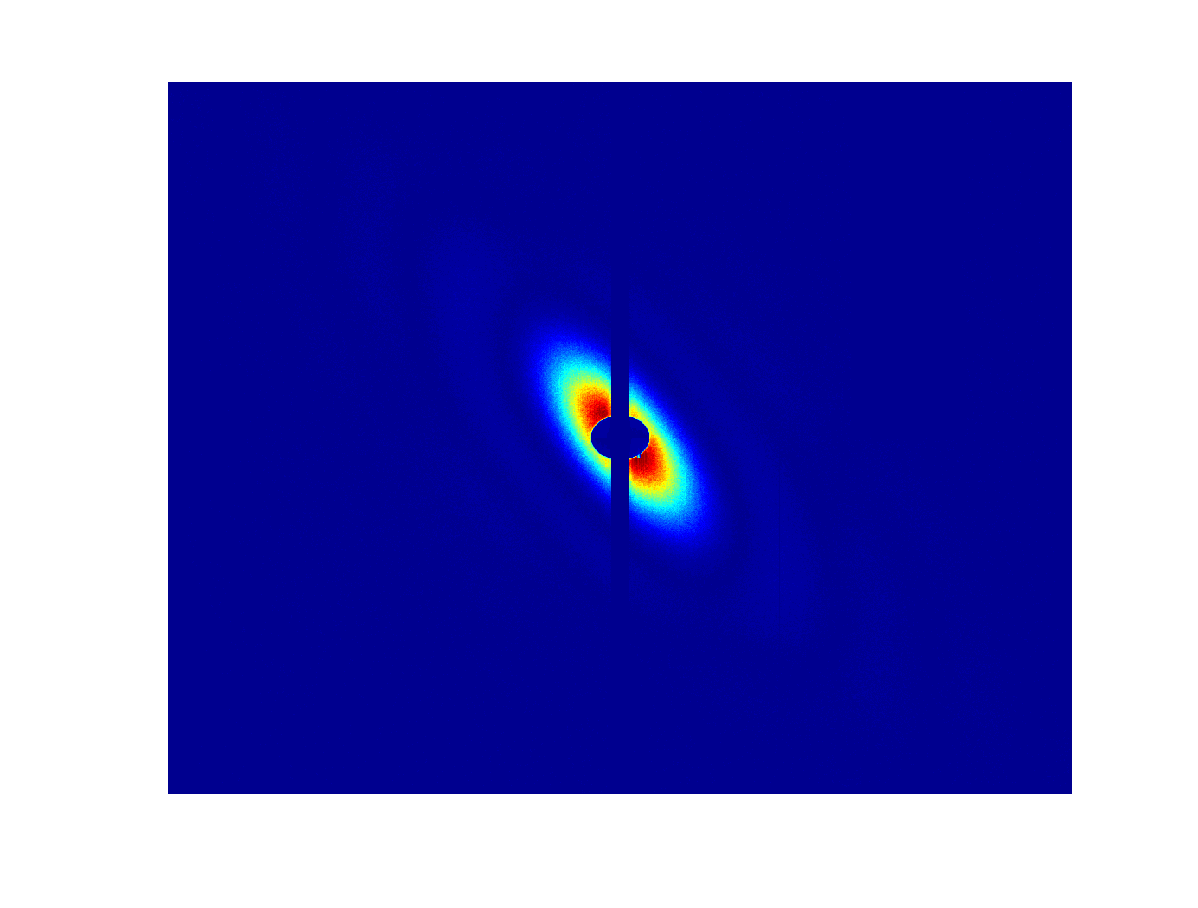
\includegraphics[width=.8\textwidth]{good1}
\end{subfigure}
\begin{subfigure}{.5\textwidth}
  \centering
  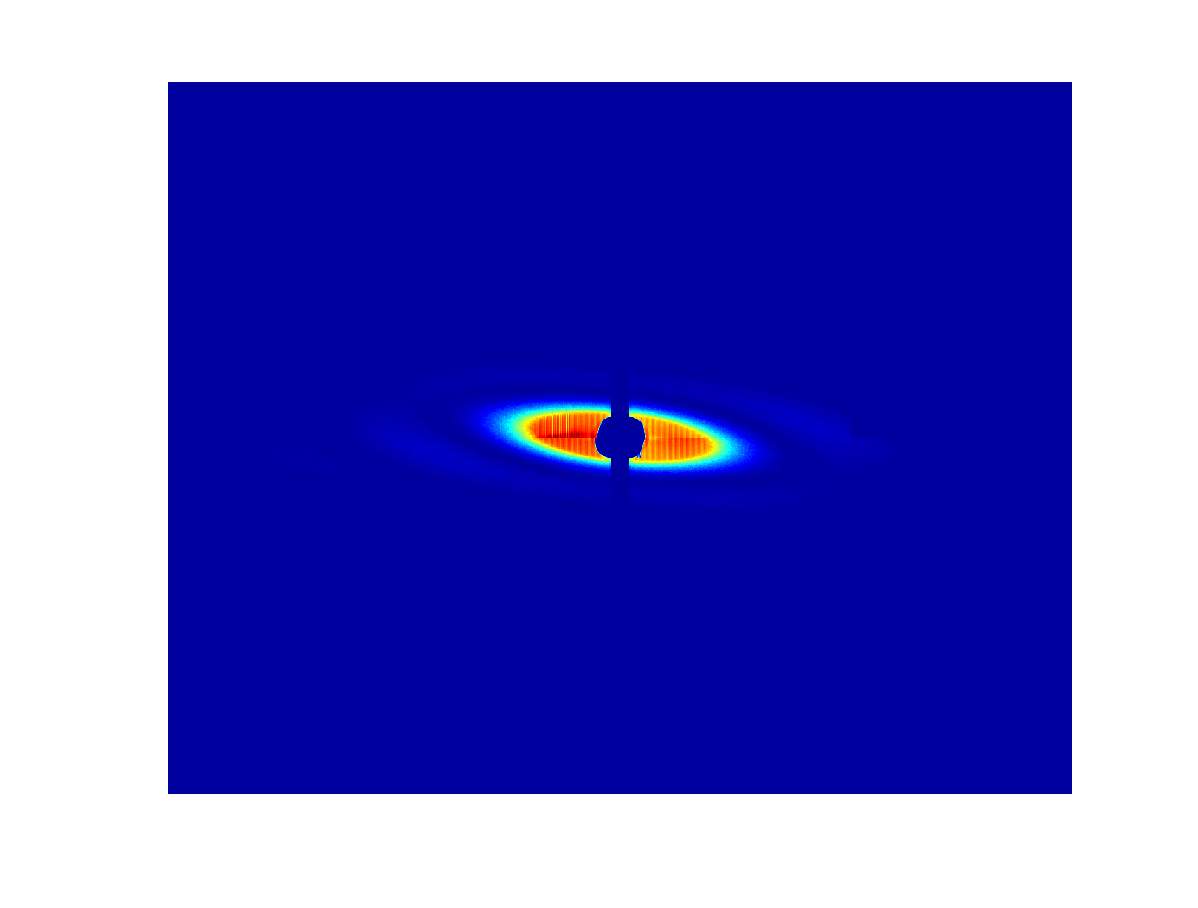
\includegraphics[width=.8\textwidth]{good2}
\end{subfigure}
\begin{subfigure}{.5\textwidth}
  \centering
  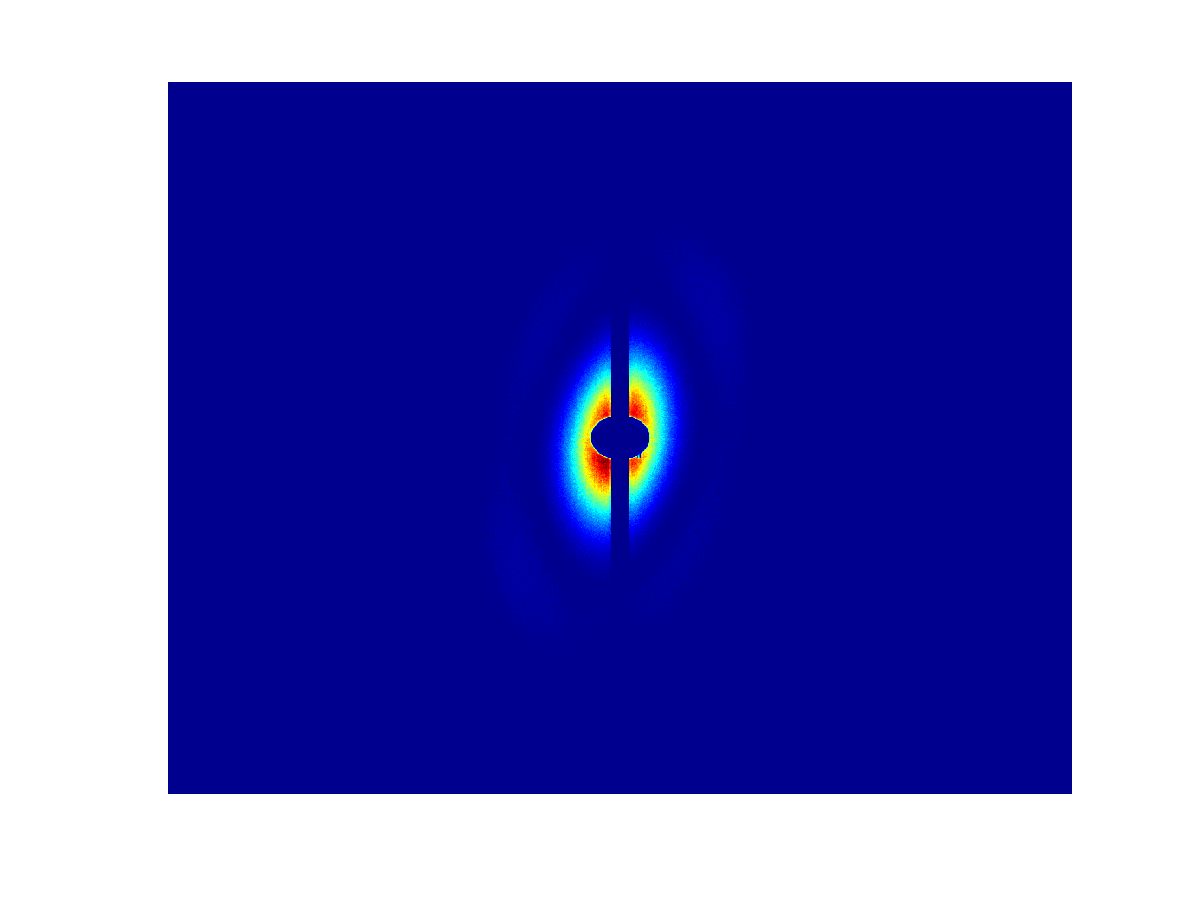
\includegraphics[width=.8\textwidth]{good3}
\end{subfigure}
\begin{subfigure}{.5\textwidth}
  \centering
  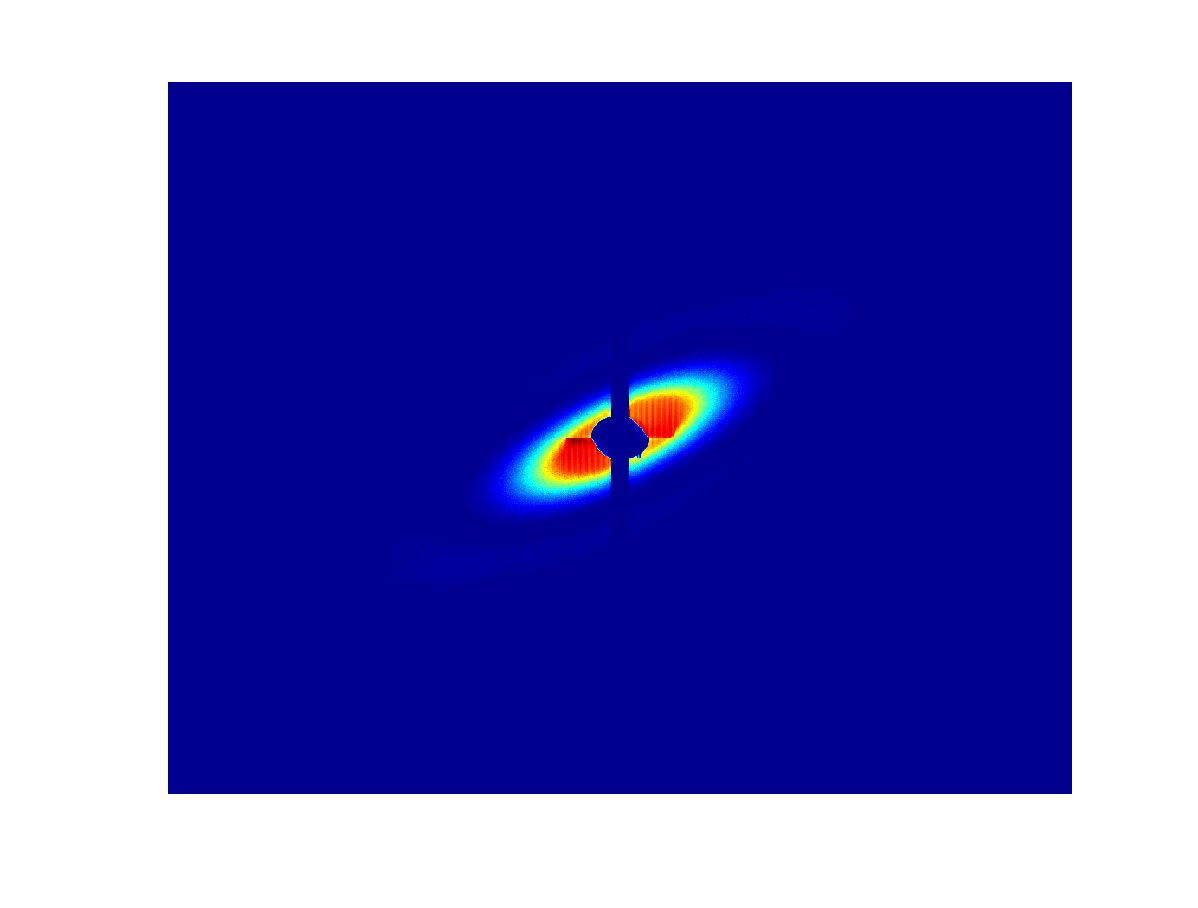
\includegraphics[width=.8\textwidth]{good4}
\end{subfigure}
\caption{Diffraction pattern that are considered as "good"}
\label{fig:gooddp1}
\end{figure}

The initial step that I did to analysis the experiment data was to separate good data from bad data. Figure \ref{fig:gooddp1} are some examples of the good data. Because it is known that the molecule is nanorice, it is expected to be close to ellipsoid. In addition to that, the diffraction patterns of ellipsoid can be easily identified. Thus, those several patterns in figure \ref{fig:gooddp1} shows the behavior where the diffracted molecules have the ellipsoidal property. Currently, by checking the data visually, I collected 200 good diffraction patterns.

\begin{figure}[ht]
\begin{subfigure}{.5\textwidth}
  \centering
  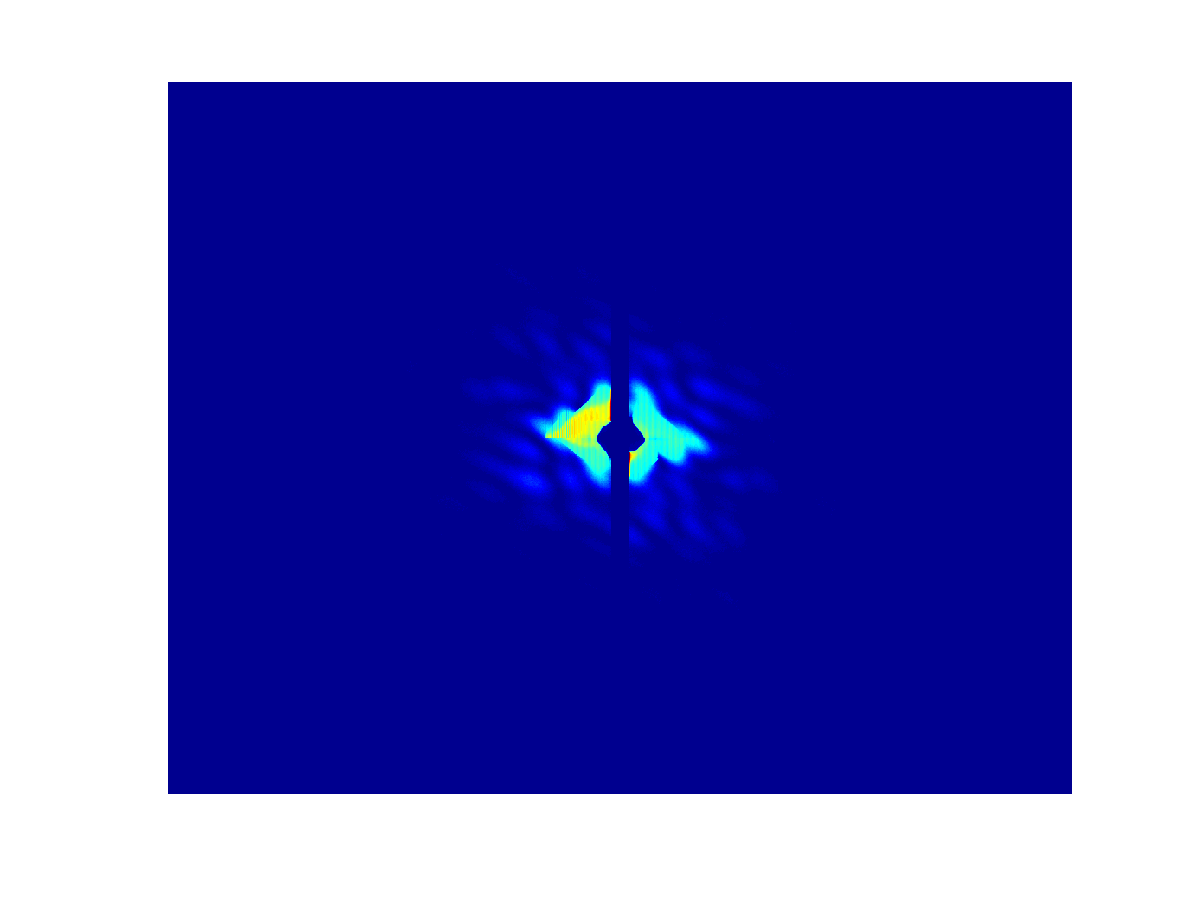
\includegraphics[width=.8\textwidth]{bad1}
\end{subfigure}
\begin{subfigure}{.5\textwidth}
  \centering
  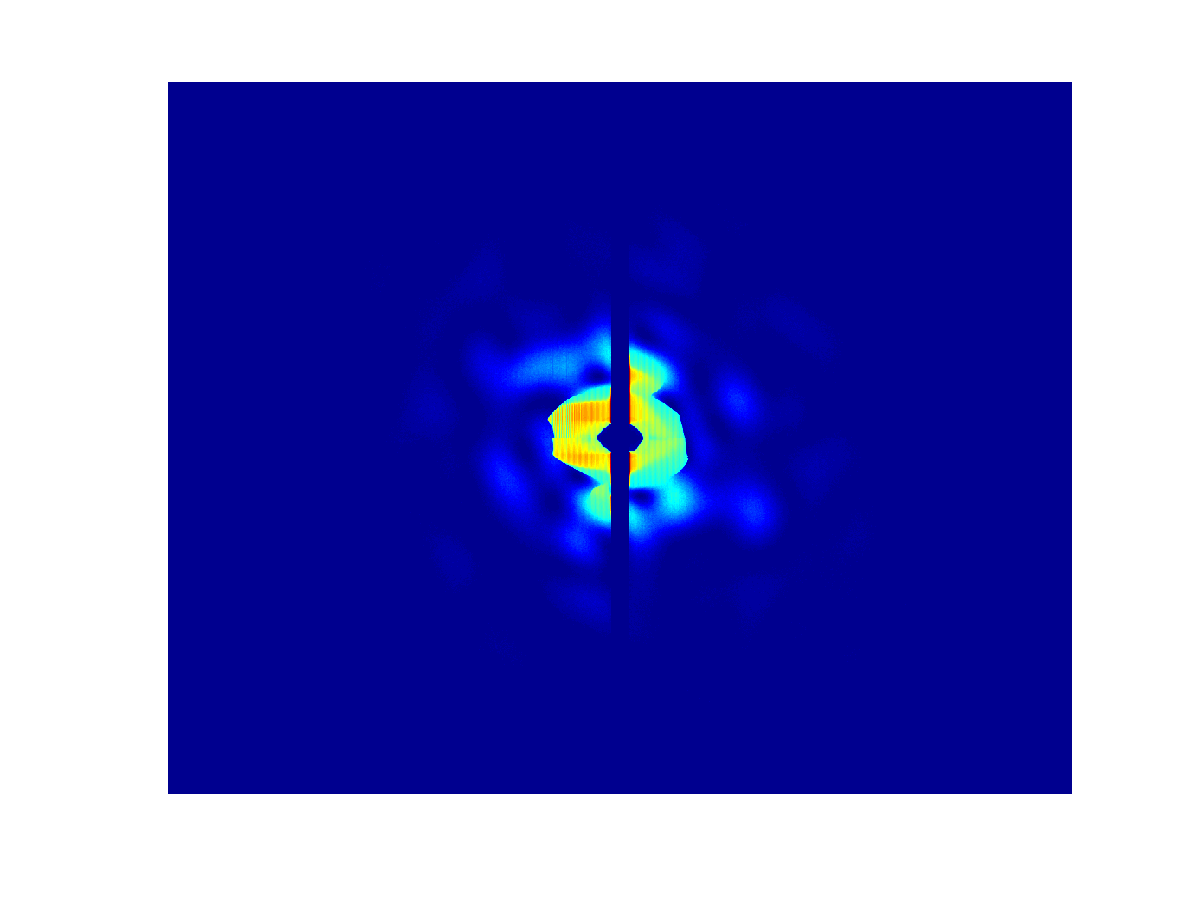
\includegraphics[width=.8\textwidth]{bad2}
\end{subfigure}
\begin{subfigure}{.5\textwidth}
  \centering
  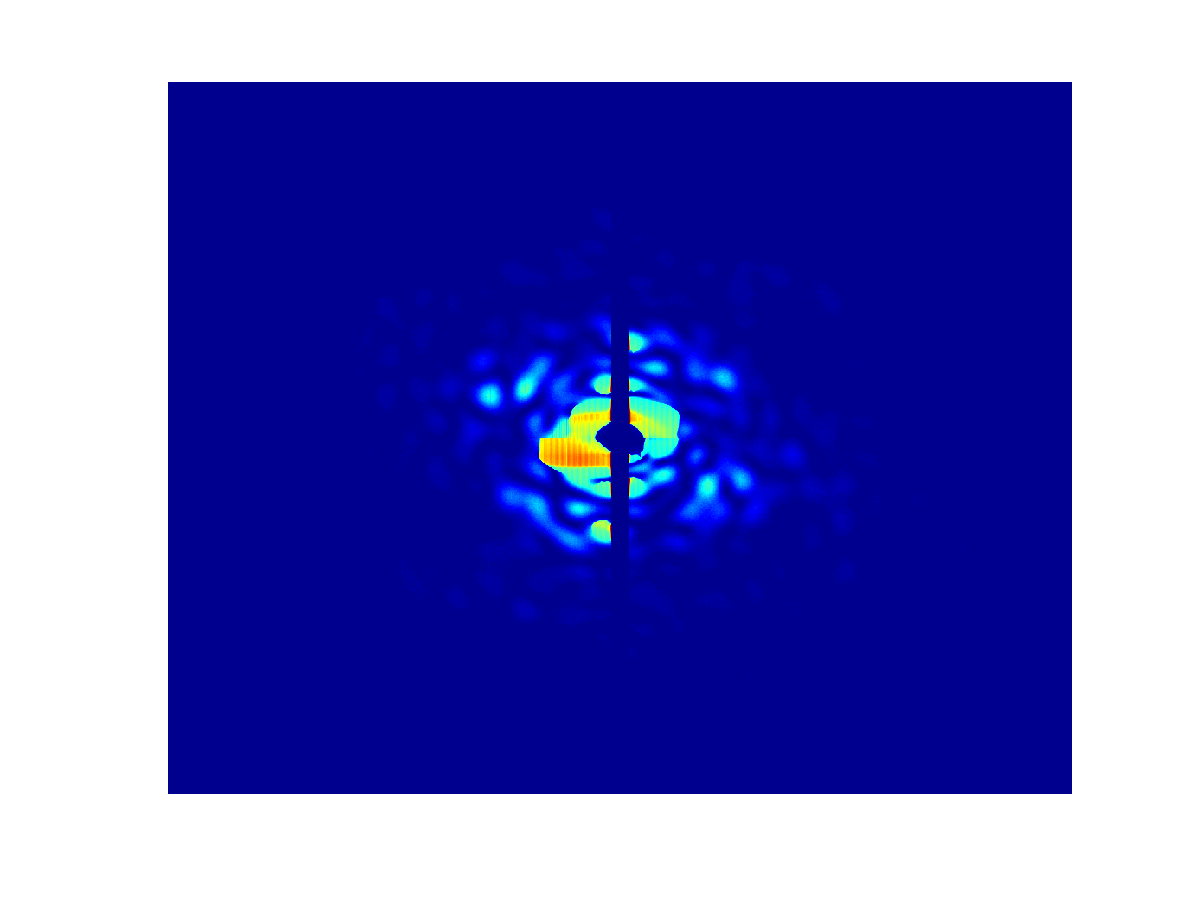
\includegraphics[width=.8\textwidth]{bad3}
\end{subfigure}
\begin{subfigure}{.5\textwidth}
  \centering
  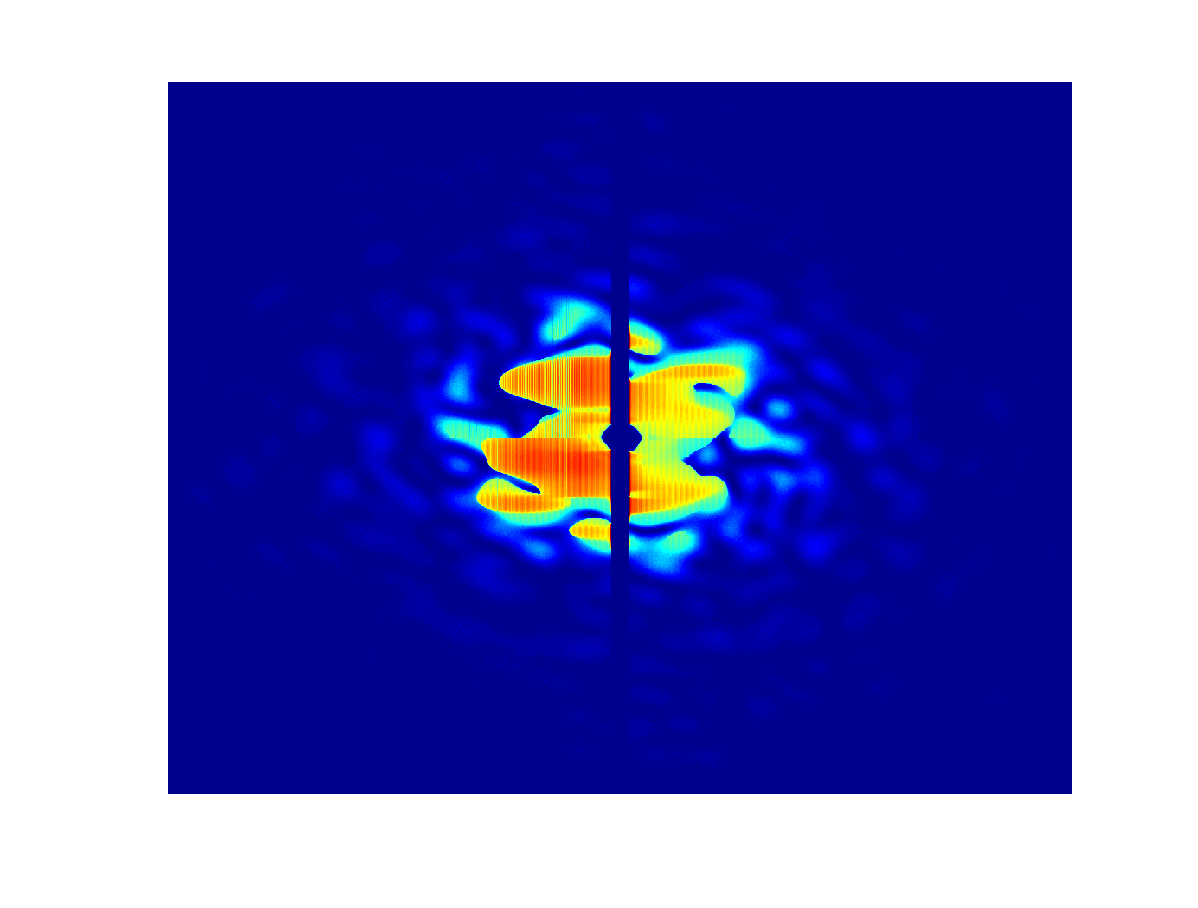
\includegraphics[width=.8\textwidth]{bad4}
\end{subfigure}
\caption{Diffraction patterns that are considered as "bad"}
\label{fig:baddp1}
\end{figure}

The exclusion bad data is simpler than finding a good one. If the diffraction patterns doesn't contain signal then they are bad data. Several example of diffraction patterns that doesn't contain strong signal is given in figure \ref{fig:baddp2}. Beside that, there is another type of bad data where the diffraction pattern doesn't seem to have ellipsoidal symmetry. Typical of those diffraction patterns are is displayed in figure \ref{fig:baddp1}. Because the nanorice in general is simple structure (close to ellipsoid), it is expected its diffraction pattern to be close to ellipsoid diffraction pattern. Thus, the diffraction pattern in figure \ref{fig:baddp1} doesn't come from the nanorice and need to be excluded for the calculation of \Blq. Given the current stage of algorithm, the algorithm need to impose azimuthal symmetry then such diffraction patterns, which doesn't show the ellipsoidal behavior, cannot be used to recover electron density. 
\begin{figure}[h]
\begin{subfigure}{.5\textwidth}
  \centering
  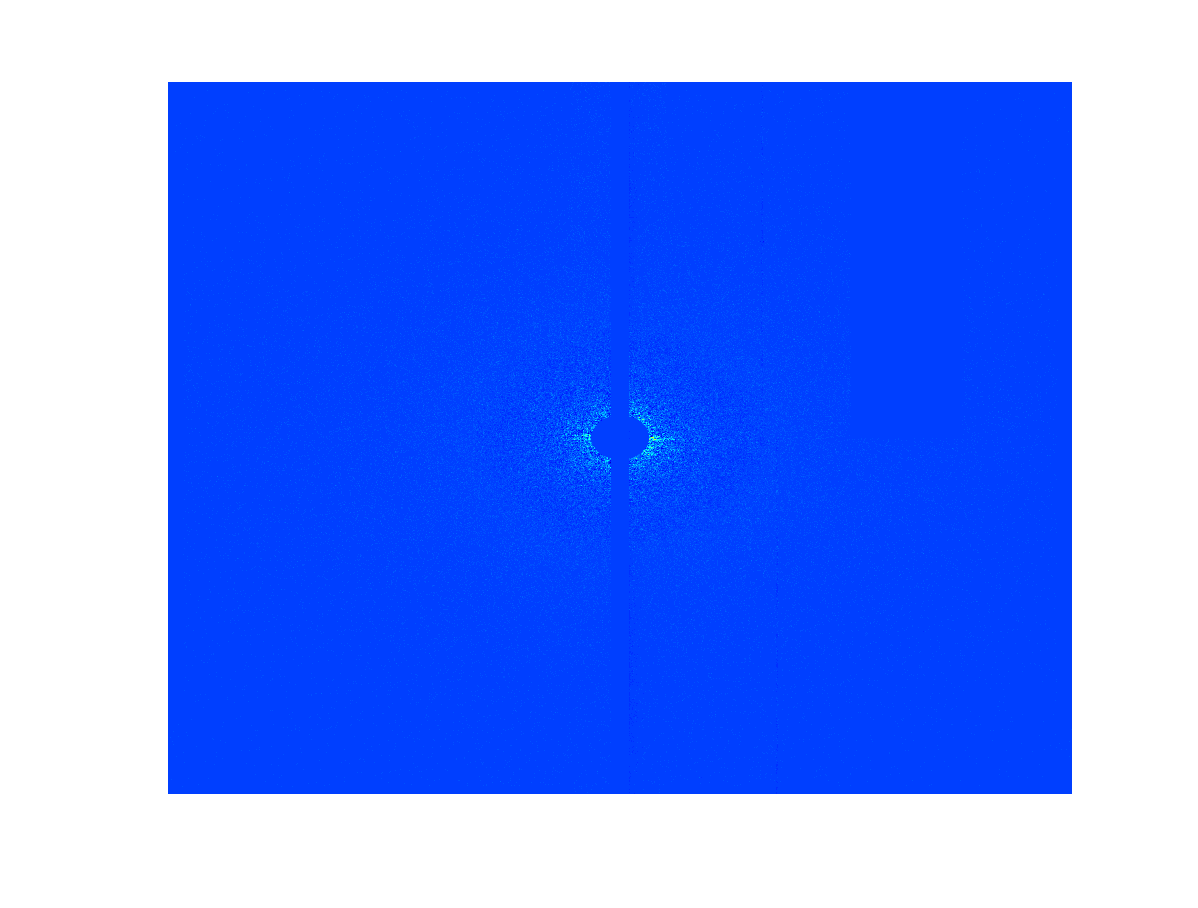
\includegraphics[width=.8\textwidth]{bad5}
\end{subfigure}
\begin{subfigure}{.5\textwidth}
  \centering
  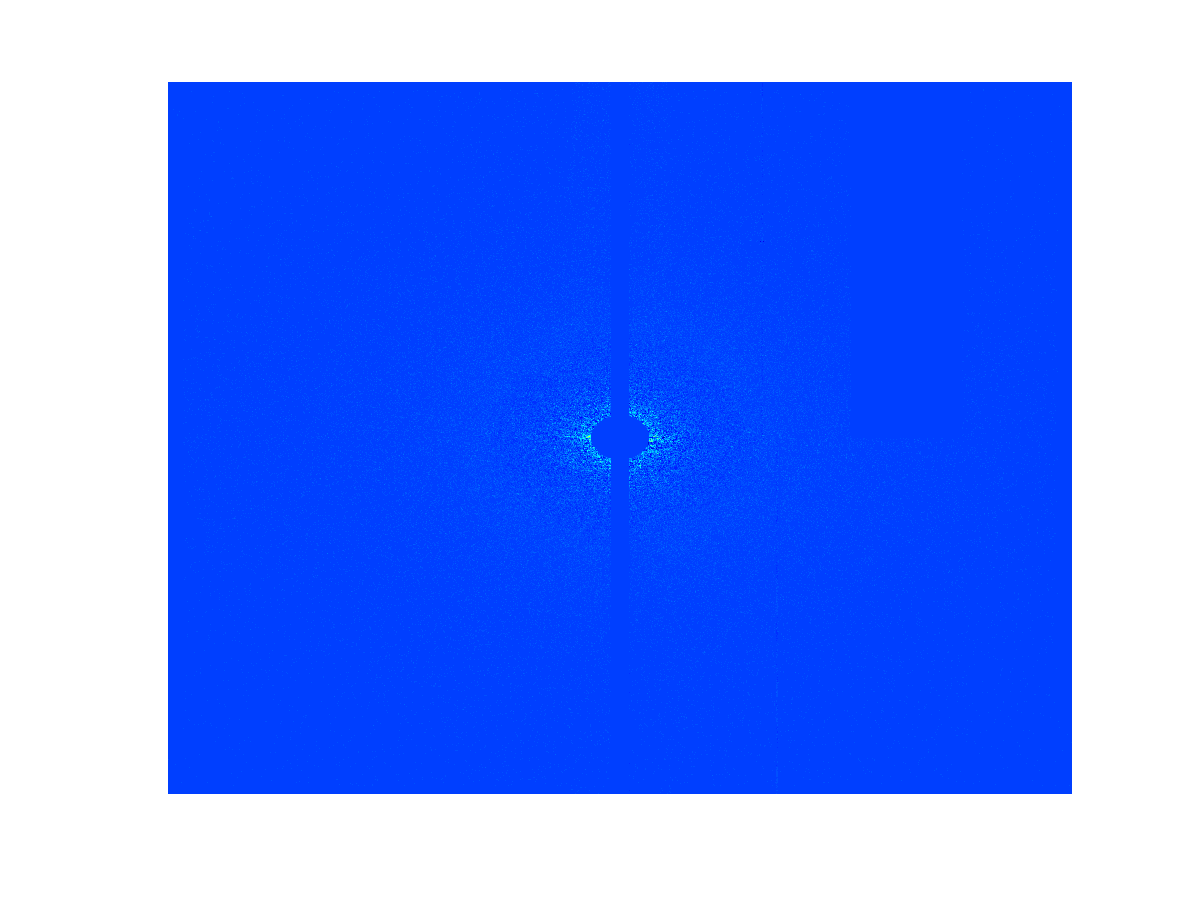
\includegraphics[width=.8\textwidth]{bad6}
\end{subfigure}
\caption{Diffraction patterns that does not contain strong scattering}
\label{fig:baddp2}
\end{figure}

After the selection of the good data was obtained, the next step was to obtain the value of each parameter in reciprocal space. To estimate the value of $dq$ (the step of reciprocal distance) for each pixel, following relation was used:
\begin{equation}
dq=\Delta_p/(\lambda Z)
\end{equation}
where $dq$ is reciprocal distance of a pixel in detector, 
$\Delta_p$ is length or size of a pixel in detector,
$\lambda$ is the wavelength used in experiment,
$Z$ is the distance from molecule to detector.
All those variables are given by this paper \cite{nanokassemeyer} where $\Delta_p=7.5\times 10^{-5}$ m, $Z=0.75$m, and $\lambda=10.38 $ \AA

After the quantity $dq$ for each pixel in detector grid was estimated, the next step was to do the interpolation from Cartesian grid into polar grid. The first step of interpolation was to specify or determine all point in polar grid. In this case, Shannon sampling was used for the radial step. The nanorice was estimated to have length 2000 \AA, therefore the radial step was $dq=1/(2D)=1/(4000) =2.5 \times 10^{-4}$ \AA. In addition to that, the angular step ($d\theta$) was taken as $2 \pi/360$. Figure \ref{fig:polargrid} show the arrangement of point in polar grid where $dq=2.5 \times 10^{-4} $  \AA and $d\theta=2 \pi/360$. 

\begin{figure}[ht]
  \centering
  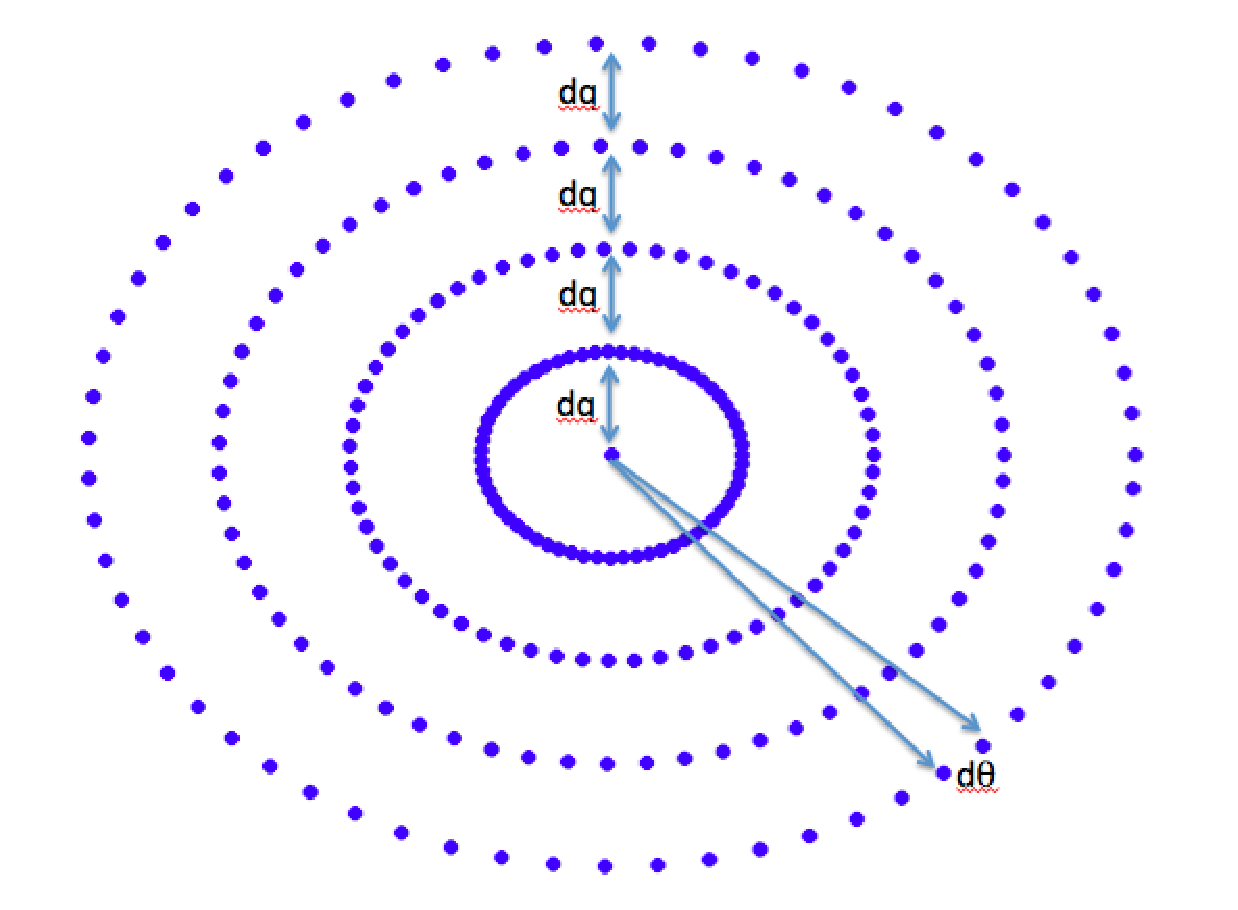
\includegraphics[width=.7\textwidth]{polargrid}
\caption{The point in polar coordinate}
\label{fig:polargrid}
\end{figure}

The scientific library in matlab was used to specify point in polar grid. The command in matlab to do the conversion is \textbf{pol2cart}. Below is an example of the code to specify point in polar grid:
\begin{lstlisting}[language=Octave]
//dq is the polar step in reciprocal space
// Nqp is the number of q point
dtheta=2*pi/360
qtheta=0:dtheta:2*pi-dtheta
qpolar=0:dq:dq*Nq          

// specify polar point in x-y form
[Xp,Yp]=pol2cart(qtheta,qpolar)  
\end{lstlisting}
The output of the code is the quantities $Xp$ and $Yp$. Those quantities represents the x-coordinate and y-coordinate of the polar grid. Thus, representation of polar grid in cartesian form can be calculated.  

The next step after determining the point in polar coordinate is to interpolate from Cartesian grid (detector grid) to polar coordinate where \Blq is defined. To get smooth function of estimation, cubic spline interpolation was used. The cubic spline interpolation divides each interval and approximates the point with third order polynomial. The polynomial is
\begin{equation}
f_{i}(x)=a_i + b_i x + c_i x^2 + d_i x^3
\label{eq:polycubspline}
\end{equation}
where subscript $i$ is the index of interval and $(a_i, b_i ,c_i , d_i)$ are the parameters needed to determined from boundary condition. The determination of the parameter used the following boundary condition:
\begin{align}
\begin{split}
f_{i}(x_{i-1})&=y_{i-1} \quad f_{i}(x_{i})=y_i \quad ,i=1,...,n \\
f'_{i}(x_i)&=f'_{i+1}(x_i) \quad i=1,...,n-1 \\
f''_{i}(x_i)&=f''_{i+1}(x_i) \quad i=1,...,n-1 
\end{split}
\label{eq:splinecond}
\end{align}  
where $y_i$ is the known function at $x_i$,  $f'_{i}(x_i)$ is the first derivative of the function and $f''_{i}(x_i)$ is the second derivative of the function. Additional two equations are needed to solve the parameters, which are called 'not-a-knot' condition. It impose condition of third derivative to be continous at two end point. Mathematically it is described as:
\begin{align}
\begin{split}
f'''_{1}(x_0)&=f'''_{2}(x_0) \quad i=1,...,n-1  \\
f'''_{n-2}(x_n)&=f'''_{n-1}(x_n) \quad i=1,...,n-1.   
\end{split}
\label{eq:splinecond2}
\end{align}
By applying the condition in equation \ref{eq:splinecond} and \ref{eq:splinecond2}, the parameters $(a_i, b_i ,c_i , d_i)$ in equation \ref{eq:polycubspline} can be found. Thus the value of the function in any point can be estimated by equation \ref{eq:polycubspline}. An example of the full derivation of the parameters is given in appendix \ref{ch:cubicspline}.  

The conversion of point in polar grid from Cartesian grid requires two dimensional interpolation. The extension from one dimensional to two dimensional is to approximate using two dimensional polynomial. The two dimensional polynomial is
\begin{equation}
f(x,y)=\sum_{i=0}^{3} \sum_{j=0}^{3} a_{ij} x^{i} y^{j}.
\label{eq:spline2d}
\end{equation}
Similar as before, coefficients $a_{ij}$ are determined from boundary condition in each interval ($i=1,...,n$),
\begin{align}
 f_{i}(x_i,y_i)=z(x_i,y_i) \quad  f_{i}(x_{i+1},y_i)=z(x_{i+1},y_i)  \\
 f_{i}(x_i,y_{i+1})=z(x_i,y_{i+1}) \quad  f_{i}(x_{i+1},y_{i+1})=z(x_{i+1},y_{i+1}) 
\end{align}
where $z(x_i,y_i)$ is the known function at $(x_i,y_i)$, the first derivative boundary
\begin{align}
&\frac{\partial f_{i}}{\partial x}\Bigr|_{x_i,y_i}=\frac{\partial f_{i+1}}{\partial x}\Bigr|_{x_i,y_i} \qquad 
\frac{\partial f_{i}}{\partial x}\Bigr|_{x_{i+1},y_i}=\frac{\partial f_{i+1}}{\partial x}\Bigr|_{x_{i+1},y_i} \\
&\frac{\partial f_{i}}{\partial x}\Bigr|_{x_i,y_{i+1}}=\frac{\partial f_{i+1}}{\partial x}\Bigr|_{x_i,y_{i+1}} \qquad 
\frac{\partial f_{i}}{\partial x}\Bigr|_{x_{i+1},y_{i+1}}=\frac{\partial f_{i+1}}{\partial x}\Bigr|_{x_{i+1},y_{i+1}} \\
&\frac{\partial f_{i}}{\partial y}\Bigr|_{x_i,y_i}=\frac{\partial f_{i+1}}{\partial y}\Bigr|_{x_i,y_i} \qquad 
\frac{\partial f_{i}}{\partial y}\Bigr|_{x_{i+1},y_i}=\frac{\partial f_{i+1}}{\partial y}\Bigr|_{x_{i+1},y_i} \\
&\frac{\partial f_{i}}{\partial y}\Bigr|_{x_i,y_{i+1}}=\frac{\partial f_{i+1}}{\partial y}\Bigr|_{x_i,y_{i+1}} \qquad 
\frac{\partial f_{i}}{\partial y}\Bigr|_{x_{i+1},y_{i+1}}=\frac{\partial f_{i+1}}{\partial y}\Bigr|_{x_{i+1},y_{i+1}} 
\end{align}
with the second derivative boundary,
\begin{align}
&\frac{\partial^2 f_{i}}{\partial x\partial y}\Bigr|_{x_i,y_i}=\frac{\partial^2 f_{i+1}}{\partial x \partial y}\Bigr|_{x_i,y_i} \qquad 
\frac{\partial^2 f_{i}}{\partial x\partial y}\Bigr|_{x_{i+1},y_i}=\frac{\partial^2 f_{i+1}}{\partial x \partial y}\Bigr|_{x_{i+1},y_i} \\
&\frac{\partial^2 f_{i}}{\partial x \partial y}\Bigr|_{x_i,y_{i+1}}=\frac{\partial^2 f_{i+1}}{\partial x \partial y}\Bigr|_{x_i,y_{i+1}} \qquad 
\frac{\partial^2 f_{i}}{\partial x \partial y}\Bigr|_{x_{i+1},y_{i+1}}=\frac{\partial^2 f_{i+1}}{\partial x \partial y}\Bigr|_{x_{i+1},y_{i+1}} \\
\end{align}


By applying the condition of continuty in the function, the first derivative and the second derivative, the parameter $a_{i,j}$ can determined in equation \label{eq:spline2d}. Thus, the value of the function in any point can be estimated by equation \ref{eq:spline2d}. 

The derivation to calculate the parameters in two dimension interpolation can be complicated. However, there are available several scientific libraries to calculate cubic spline interpolation. The library that I used to convert Cartesian grid into polar grid was matlab libray under the command \textbf{interp2}. A snippet of the code to use \textbf{interp2} is shown below:
\begin{lstlisting}[language=Octave]
//dqc is the reciprocal distance per pixel
// N is the number of pixel in one dimension divided by 2
[Xc,Yc]=meshgrid(-N*dqc:dqc:N*dqc,-N*dqc:dqc:N*dqc)                                        

//dq is the polar step in reciprocal space
// Nqp is the number of q point
dtheta=2*pi/360
qtheta=0:dtheta:2*pi-dtheta
qpolar=0:dq:dq*Nq          

// specify the polar point in x-y form
[Xp,Yp]=pol2cart(qtheta,qpolar)  

//Do the interpolation 
// F is the known value in each cartesian point
// V is the diffraction pattern in polar point
V=interp2(Xc,Yc,F,Xp,Yp,'spline')
\end{lstlisting}
The output of the code is the quantity $V$ where it hold the value of interpolation in polar grid. Thus, a set of new polar diffraction patterns can be obtained with the cubic spline interpolation. 

After the diffraction patterns were sampled in polar point, the calculation of the angular pair correlation can be done. The pair correlation do the sum over all diffraction patterns and correlate them in angularly. Formula in equation \ref{eq:crosscor} was used to calculate $C_{2}$ where  $I(q,\phi)$ is the diffraction pattern in polar grid and $(q,\phi)$ are the point in polar grid. Subsequent to that, \Blq was calulated using matrix inversion in equation \ref{C2definition}. As a result of that, \Blq from the experiment data of nanorice could be determined.   

It is important to note that, the derivation to get \Blq from equation \ref{eq:crosscor} to equation \ref{C2definition} use fundamental assumption where all random angle span through all possible angle (equation \ref{eq:orthotheorem}). However, there are only 200 good diffraction patterns available from the experimental data. That is why it is important to check the convergence of \Blq from 200 diffraction patterns.    

The matrices \Blq were calculated from 200 diffraction patterns of nanorice. Subsequent to that, SVD on the \Blq was performed for each $l$ and its nonzero singular value is displayed in figure \ref{fig:svdnanoexp}

It is shown in the plot that all the matrices \Blq, which correspond to $l$, have singular values more than $2l+1$. In other words, the plot shows the behavior more asymmetric than an asymmetric pattern, which is not plausible. The only explanation is that the \Blq is not in the form of dot product. As explained earlier, if \Blq is a form of dot product then the SVD on \Blq will have singular values less than or equal to the asymmetric pattern, which is $2l+1$. In conclusion, the \Blq calculated from 200 diffraction pattern of nanorice doesn't converge to its theoritical value. 

\begin{figure}[h!]
  \centering
  \includegraphics[width=.8\textwidth]{svdBnanoexp}
\caption{The number of nonzero singular value is more than $2 l+1$. The data doesn't show the convergence of \Blq}
\label{fig:svdnanoexp}
\end{figure}

Before using the \Blq for structure determination, checking accurate convergence is priority. Here one way to check the convergence is known by using SVD on the \Blq. If it is found than the number of singular values of \Blq is higher than those from asymmetric pattern then additional steps to correct the \Blq is needed. 


%CHAPTER 3 Convergence Limit
\clearpage
\section{Convergence Limit} \label{sec:convlim}
From eq. \ref{eq:crosscor} , the derivation from $C_2$ to $B_{l}(q,q')$ uses the fundamental assumption that the collection of random angle spans through all members of rotational group.
SO(3) or 3D rotational group have an infinite number of members that are specified by 3 different angles $\alpha$, $\beta$, and $\gamma$.
The experiment is capable to produce only a finite number of the diffraction patterns.
 There is a sort of incompatibility between the finite number of the diffraction patterns from experiment and the assumption that all infinite number of members of rotational group must be satisfied.
Thus, It is fundamental to find the limit of how the correlation can be used for a finite number of diffraction patterns only.

One can expect at a particular finite number of the diffraction patterns, the calculated $B_{l}(q,q')$  will converge enough to theoritical $B_{l}(q,q')$, which is obtained from infinite number of the diffraction patterns.
 In order to find the limit, a collection of diffraction patterns is simulated. 
There are two different structure compared. First model is PBCV (Paramecium bursaria chlorella)\cite{RossmanPBCV}. It is used as model, which has icosahedral symmetry and the electron density is calculated from pdb(1m4x). Second model is Photoactive yellow protein (PYP) and the electron density is calculated from pdb(2phy) \cite{pyppaper}.
 PBCV is a structure that has 60 rotational symmetry elements whereas pyp doesn't have rotational symmetry at all.
 The two different structures that contain different type of symmetry should be able to tell what is the effect of symmetry on the convergence of $B_{l}(q,q')$. Because $B_{l}(q,q')$ consist of expansion of spherical harmonics of the intensity, the value of $l$ correspond to $q_{max}$, which is directly related to resolution in real space\cite{saldinvirus}.
 By plotting for different value of $l$'s, comparison of how convergence of $B_{l}(q,q')$ affect resolution is studied.

The diffraction patterns is a 2D slice of the intensity in reciprocal space. The random angle diffraction patterns are simulated by calculating the intensity from the model and randomly take the 2D slice of intensity. 
\begin{figure}[h]
\begin{subfigure}{.5\textwidth}
  \centering
  \includegraphics[width=.8\textwidth]{dppbcv}
  \caption{PBCV (Paramecium bursaria chlorella)}
\end{subfigure}
\begin{subfigure}{.5\textwidth}
  \centering
  \includegraphics[width=.8\textwidth]{dppyp}
  \caption{PYP (Photoactive yellow protein)}
\end{subfigure}
\caption{A noise free diffraction pattern in random orientation}
\label{fig:simdp}
\end{figure}
Typical diffraction pattern from PBCV and PYP are displayed in figure \ref{fig:simdp}. It is easily recognized that the diffraction pattern from PBCV is from a symmetrical object whereas the diffraction pattern from PYP doesn't have an indication of symmetry. 

\begin{figure}[h]
\begin{subfigure}{.5\textwidth}
  \centering
  \includegraphics[width=.8\textwidth]{convpypl6}
  \caption{\Blq for $l=6$}
  \label{fig:convpypl6}
\end{subfigure}
\begin{subfigure}{.5\textwidth}
  \centering
  \includegraphics[width=.8\textwidth]{convpypl12}
  \caption{\Blq for $l=12$}
\end{subfigure}
\caption{Convergence of \Blq from a set of noise free diffraction patterns of PYP}
\label{fig:convpyp}
\end{figure}

The convergence of \Blq can be analyzed by comparing three different sets of simulated diffraction patterns. From figure \ref{fig:convpyp}, there are curves of \Blq that are calculated from 10, 100, and 1000 random noise free diffraction patterns. The curves are represented by solid lines. The dashed lines are the curves of \Blq calculated from infinite number of diffraction pattern. The solid lines are expected to converge into the dashed line for a large number of diffraction patterns.  

From figure \ref{fig:convpyp}, the dashed line coincides with the solid line when the number of diffraction pattern reach 1000. Two \Blq curve are calculated, one for $l=6$ and the other for $l=12$. Both of them show that the convergence is reached by only using 1000 diffraction patterns.

Eventhough the theory explicitly assume the requirement of infinite number of the diffraction patterns, the simulation shows that only 1000 diffraction patterns are enough to approximate the theoretical value of \Blq. The 1000 diffraction patterns indicate the feasibility of the correlation method to be used to recover the electron density.
\begin{figure}[h]
\begin{subfigure}{.5\textwidth}
  \centering
  \includegraphics[width=.8\textwidth]{convpbcv6}
  \caption{\Blq for $l=6$}
  \label{fig:sub1}
\end{subfigure}
\begin{subfigure}{.5\textwidth}
  \centering
  \includegraphics[width=.8\textwidth]{convpbcvl12}
  \caption{\Blq for $l=12$}
  \label{fig:sub2}
\end{subfigure}
\caption{The Convergence of \Blq from a set of noise free diffraction patterns of PBCV}
\label{fig:convpbcv}
\end{figure}

From figure \ref{fig:convpbcv}, the dashed line coincides with the solid line when number of the diffraction patterns reach 100. Two \Blq curves are calculated, one for $l=6$ and $l=25$. Both of them show the convergence is reached by only 100 diffraction patterns. In contrast to the figure \ref{fig:convpyp}, the convergence is reached by a significant smaller set of diffraction patterns. The model of figure \ref{fig:convpbcv} is PBCV, which has 60 different rotational symmetry. It is apparent from the graph that rotational symmetry reduces the total diffraction patterns needed to converge to theoretical value.     

The repetition or symmetry of particle is the reason for particle having less independent parameters. In the case of rotational symmetry, the diffraction pattern doesn't change if symmetric particle is rotated with respect to the axis of symmetry. The likelihood of having exact same diffraction pattern by rotation of random angle will increase if the particle has higher rotational symmetry. This explains the decline of the convergence of \Blq when the particle is PBCV since it has 60 rotational symmetry. 

The convergence is an important indication of properly calculated \Blq from experimental diffraction patterns. In experiment, different sets of diffraction patterns can be collected. By adding a higher number of diffraction patterns, the 2 largest set of diffraction pattern should have smaller difference because those curve nearly converge each other. It is expected that the experiment data will have higher number of diffraction patterns to converge compared to simulation. Eventhough the number of diffraction patterns needed for convergence currently is unknown for the experimental data, the convergence is necessary condition to be calculated. If convergence is not achieved, more diffraction patterns are needed for that particular structure.      

It is possible if the experimental data contain data which are dominated by noise. The inclusion of bad data in \Blq calculation will prevent the curve of \Blq vs $q$ from converging. If the portion of bad data is insignificant, it has little effect on \Blq and the convergence will be satisfied. However, whenever the bad data is significant enough in the collection of diffraction patterns, the convergence of \Blq cannot be achieved. The convergence of \Blq is important indication to observe whether bad data is present in the collection of random diffraction patterns. Provided that the convergence of \Blq is not achieved, the presence of bad data can be one of the reason therefore further effort to exclude those should be performed.

Assuming bad data is not present but convergence is not achieved, information about distribution of orientation of diffraction patterns can be deduced. Theoretically, orientation should be random or span through all angle. 
It is possible that the randomness of the orientation of the diffraction patterns is not enough to span through uniform angles. Another important point is by observing non-converging \Blq, there is possibility that the diffraction patterns have orientation tendency which is not uniform. It will give clear insight how the experiment process occur. 

This section cover the importance of the convergence of \Blq that are calculated from the collection of the diffraction patterns. The demonstration of converging \Blq is performed by using two models namely PBCV and PYP. The feasibility of the correlation method is verified by showing that only 1000 diffraction patterns of asymmetrical molecule converge into theoretical \Blq. Furthermore, the possibility of nonconverging \Blq from a set of experimental data is discussed. In conclusion, the convergence of \Blq is vital tool for analyzing experimental data and it is the first step that need to be confirmed. 




% CHAPTER 4 Section 2D Case
\clearpage
\chapter{Reconstruction}
\section{2D Case} 
\label{sec:2Dcase}
\subsection{Polar Fourier Transform}
As mentioned in the previous section, several experiments produce diffraction patterns along azimuthal axis. There is only one unknown orientation angle in the collection of diffraction patterns. The independent orientation is rotation with respect to azimuth axis. 

The algorithm explained below will mainly focus on how to get general 2D projected structure from \Bmq. The construction of \Imq from \Bmq leave phases, which is nonunique \cite{saldin2010PhysB}. The information about the phases can be gotten by constraining the structure and the intensities as real-positive quantities. That information provides additional information from \Bmq to \Imq.

Phasing is an algorithm to find the structure from the missing phases of intensities. The way it works is by constraining any information about structure. The condition of electron density must be positive and real is imposed. In addition to that, several algorithms impose structure to be localized. Phasing is one of established algorithm that works by constraining prior information throughout iteration. A Similar method can be applied to impose a real space constraint iteratively in order to get structure from \Bmq.  

By definition, \Bmq is described in polar coordinate \cite{saldinNJournal}. To avoid interpolation, polar coordinate is chosen as a basis coordinate for real space and reciprocal space. The consequence of that it excludes FFT algorithm to be used inside iteration because FFT is defined in cartesian coordinate. The calculation of polar fourier transform is required and need to be formulated to go back and forth from real and reciprocal space. 

Any function can be decomposed into its basis function component. It is sensible to decompose function into its exponential components because the problem is related to the rotation of azimuthal angle. The decomposition of the electron density of the molecule is defined by
\begin{eqnarray}
\label{eq:rhorm}
\rho(r,\theta)=\sum_{m} \rho_{m}(r) \exp(i m \theta)
\end{eqnarray}
where $r$ and $\theta$ refer to a coordinate that can be sampled at polar point without interpolation. $\rho_{m}$ contain only radial dependence and the angular dependence is contained in $m$ components. 

Intensity is absolute square of Fourier transform of the electron density. The established FFT routines cannot be used owing to the fact that $\rho$ are sampled at polar coordinate. It is necessary to obtain a direct relation from electron density to intensity directly in polar coordinate. Fourier transform of $\rho(r,\theta)$ is shown below:
\begin{eqnarray}
\label{Aqpolarfourier}
A(\vec{q}) = \int d^{2}r \rho(r,\theta) \exp(i \vec{q} \cdot \vec{r}).  
\end{eqnarray}

In general, the structure factor is a fourier transform of electron density. As stated in equation \ref{Aqpolarfourier}, the structure factor is obtained by integrating over all electron density multiplied by a phase factor. All point are sampled in polar coordinates for both the electron density $(r,\theta)$ and the structure factor $(q,\theta_{q})$. 

One can relate exponential functions to Bessel function. The relation is called Jacobi Anger relation, which express exponential function into a sum of Bessel functions \cite{jacobianger}. The relation is
\begin{eqnarray}
\label{jacobanger}
\exp(i \vec{q} \cdot \vec{r} ) &=& \exp(i q r \cos( \theta_{q}-\theta_{r} ))  \\
&=& \sum_{m} i^{m} J_{m}(q r) \exp(i m ( \theta_{q}-\theta_{r} ) ). 
\end{eqnarray}
By substituting the Jacobi-Anger expansion into the Fourier transform of the electron density, a relation between structure factor, electron density and Bessel function is obtained: 
\begin{eqnarray}
\label{Amderive}
A(\vec{q}) &=& \int d^{2}r \rho(r,\theta) \exp(i \vec{q} \cdot \vec{r})  \\ 
&=& \int d^{2}r \sum_{m} \rho(r,\theta) i^m J_{m}(q r) \exp(i m ( \theta_{q}-\theta_{r} )).
\end{eqnarray}

\Bmq can be expressed in terms of an exponential decomposition of the intensity. By substituting equation \ref{rhom} into equation \ref{Amderive}, the structure factor can be expressed in terms of exponential decomposition. The derivation is shown below:
\begin{eqnarray}
\label{Amderive2}
A(\vec{q})&=& \int d^{2}r \sum_{m} \bigg[\sum_{m'} \rho_{m'}(r) \exp(i m' \theta_{r}) \bigg] i^m J_{m}(q r) \exp(i m ( \theta_{q}-\theta_{r} )) \\
&=& \int r dr \sum_{m',m} \rho_{m'}(r) i^m J_{m}(q r) \exp(i m ( \theta_{q})) \int d\theta_{r} \exp(i (m'-m) \theta_{r}).
\end{eqnarray}

Equation \ref{Amderive2} involve infinite integral of the exponential function. That integral is equivalent to the delta function \cite{deltafunction}, hence equation \ref{Amderive2} can be simplified become
\begin{eqnarray}
\label{deltafun}
\delta(m'-m)=\frac{1}{2 \pi} \int_{\infty}^{-\infty} \exp(i x(m'-m)) dx .
\end{eqnarray}
Thus, equation \ref{Amderive} can be written as
\begin{eqnarray}
\label{Amderive3}
A(\vec{q}) = \int r dr \sum_{m} \rho_m(r) i^m J_{m}(q r) 2 \pi \exp(i m ( \theta_{q})) . 
\end{eqnarray}
By decomposing left hand side of equation \ref{Amderive3} and equating each component in exponential term, a new relation is found that is 
\begin{eqnarray}
\sum_{m} A_{m}(q) \exp(i m \theta_{q}) = \sum_{m} \bigg[ 2 \pi \int r dr \rho_{m}(r) i^{m} J_{m}(q r) \bigg] \exp(i m \theta_{q}).  
\end{eqnarray}
The important relation between the structure factor decomposition and its exponential components can be obtained:
\begin{eqnarray}
\label{Am}
A_{m}(q) &=& 2 \pi \int rdr  \rho_{m}(r) i^m J_{m}(q r) .
\end{eqnarray}

In a similar way as the Fourier transform, the inverse Fourier transform is obtained by swaping $i$ to $-i$. It is generally accepted that electron density is the inverse Fourier transform of the structure factor. By using equation \ref{jacobanger} and equation \ref{deltafun}, the derivation is performed in the same way as polar Fourier transform. The following is the derivation:
\begin{eqnarray*}
\rho(\vec{r}) &=& \int d^{2}r A(q,\theta_{q}) \exp(-i \vec{q} \cdot \vec{r})  \\
&=& \int d^{2}q \sum_{m} A(q,\theta_{q}) (-i)^m J_{m}(q r) \exp(-i m ( \theta_{q}-\theta_{r} )) \\
&=& \int d^{2}q \sum_{m} \bigg[\sum_{m'} A_{m'}(q) \exp(i m' \theta_{q}) \bigg] (-i)^m J_{m}(q r) \exp(-i m ( \theta_{q}-\theta_{r} )) \\
&=& \int q dq \sum_{m',m} A_{m'}(q) (-i)^m J_{m}(q r) \exp(i m ( \theta_{r})) \int d\theta_{q} \exp(i (m'-m) \theta_{q}) \\
&=& \int q dq \sum_{m} A_m(q) (-i)^m J_{m}(q r) \exp(i m ( \theta_{r})) 2 \pi \\
\sum_{m} \rho_{m}(r) \exp(i m \theta_{r}) &=& \sum_{m} \bigg[ 2 \pi \int q dq A_{m}(q) (-i)^{m} J_{m}(q r) \bigg] \exp(i m \theta_{r}). 
\end{eqnarray*}
Because now the left hand side and the previous right hand side of the equation have the exponential terms, equating each component will lead to a new important equation. The relation between the exponential components of the electron density and the exponential component of the structure factor can be obtained: 
\begin{eqnarray}
\label{rhom}
\rho_{m}(r) &=& 2 \pi \int qdq  A_{m}(q) (-i)^m J_{m}(q r).
\end{eqnarray}

Equations \ref{Am} and \ref{rhom} are the foundation to do Fourier transform in polar coordinates directly without involving the cartesian space. After obtaining the exponential components of the structure factor or the electron density, the summation with respect to its basis function is performed to get $\rho(\vec{r})$ or $A(\vec{q})$ as shown
\begin{eqnarray}
\label{rho_aq}
\rho(\vec{r})&=&\sum_{m} \rho_{m}(r) \exp(i m \theta)  \\
A(\vec{q})&=&\sum_{m} A_{m}(q) \exp(i m \theta). \nonumber 
\end{eqnarray}

\subsection{Angular Correlation Constraint}
As explained earlier, the correlation methods need to calculate \Bmq from experiment. Information of intensity should be obtained from \Bmq and the other constraints. Phasing algorithm can be modified so that the constraint is on \Bmq instead of intensity\cite{Donatelli}. The step is explained as follow:
\begin{figure}[ht]
  \centering
  \includegraphics[width=.8\textwidth]{Bconstraint}
\caption{Full cycle of phasing algorithm with $B_{m}(q,q)$ as constraint}
\label{fig:Bconstraint}
\end{figure}
\begin{enumerate}
  \item Start initial guess of $\rho(\vec{r})$
  \item Calculate $\rho_{m}(q)$ from $\rho(\vec{r})$
  \item Use equation \ref{Am} to calculate $A_{m}(q)$
  \item Calculate $I_{m}(q)$ from $A_{m}(q)$ and keep information of phase. \\
    Start from calculating $A(\vec{q})=\sum_{m} A_{m}(\vec{q}) \exp(i m \theta)$ then $I(\vec{q})=|A(\vec{q})|^{2}$. \\
    Final step is $I_{m}(q)=\int I(\vec{q}) \exp(-i m \theta) d\theta $ 
  \item Project $I_{m}(q)$ to satisfy $B_{m}(q,q)$ constraint
  \item Use phase from step 4 to obtain $A'_{m}(q)$ 
  \item Calculate $\rho_{m}(q)$ from equation \ref{rhom}
  \item Use HIO, ER, and shrinkwrap to constraint $\rho(\vec{r})$ and cycle is repeated
\end{enumerate}
\begin{figure}[ht]
  \centering
  \includegraphics[width=.3\textwidth]{kc2dmodel}
\caption{ Electron density of K channel protein is used as a model to calculate $B_{m}(q,q)$}
\label{fig:kc2dmodel}
\end{figure}
\begin{figure}[ht]
  \centering
  \includegraphics[width=.27\textwidth]{kc2drec}
\caption{Reconstruction of electron density by only constraining to diagonal value of $B_{m}(q,q)$}
\label{fig:kc2drec}
\end{figure}
Figure \ref{fig:kc2dmodel} is model that is used simulate $B_{m}(q,q)$. 
After applying phasing constraint on $B_{m}(q,q)$, the reconstruction is shown on figure \ref{fig:kc2drec}. 

Important to note that in this reconstruction only information on diagonal value of $B_{m}(q,q)$ is used.  
Another important quantity is R-factor, R-factor between \Bmq model and its reconstruction is $0.15$, which is defined as
\begin{eqnarray}
R_{factor}=\frac{\sum ||B_{m}(q,q)|-|B_{m}(q,q)_{exp}||}{\sum |B_{m}(q,q)_{exp}|}. 
\end{eqnarray}
Judging from figure \ref{fig:kc2drec} and R-factor, the reconstruction is reasonable enough even though only diagonal values are used as constraint. The discrepancy between model and reconstruction could be attributed to the fact that only diagonal values of $B_{m}(q,q)$ are used. 



% CHAPTER 4 Section Triple Correlation
\section{Triple Correlation}\label{sec:triple}
Apart from \Blq, triple correlation, which can be calculated from squaring one term in pair correlation, also can be used to reconstruct the electron density. Since triple correlation is more complicated than \Blq, only the case which has azimuthal property is considered in this section.

In this section, a method to recover azimuthal electron density from an ensemble of random angle diffraction patterns is explained. The method is developed to recover electron density of nanorice. Moreover, experimental diffraction patterns is readily available and can be downloaded from cxidb.org. \cite{nanokassemeyer}

\begin{figure}[h!]
\centering
 \includegraphics[width=.3\textwidth]{ellipsdot}
\caption{ 3D ellipsoidal cartesian grid is used as model}
\label{fig:ellipsdot}
\end{figure}

The object under study is nanorice,which has an ellipsoid shape. For an initial model of nanorice we assumed an ellipsoid on a 3D cartesian grid in real space. We took the electron density of the nanorice particle to be 1 inside and zero outside the ellipsoid. This model is shown on Figure \ref{fig:ellipsdot} . Subsequently random angle diffraction patterns can be simulated.

The first step of simulation by calculating the structure factor. The structure factor is calculated in reciprocal space using the Fourier transform of the model. The calculation of structure factor and the intensity is
\begin{eqnarray}
A(\hat{q}) &=& \sum_{j} \rho (\hat{r}_{j}) \exp(2 \pi \hat{q}.\hat{r}_{j}) \\
I(\hat{q})&=&|A(\hat{q})|^2. 
\end{eqnarray}
After the intensity is obtained, its spherical harmonics expansion are calculated by integrating the intensity times spherical harmonics over all angles on surface area. Mathematically, the calculation is expressed as 
\begin{eqnarray}
I_{lm}(q) = \int I(q,\theta,\phi) Y_{lm}^{*}(\theta,\phi) d\Omega. 
\label{Ilm}
\end{eqnarray}
Now, random rotation of $I_{lm}$ is performed by multiplying the $I_{lm}$ by rotation matrix. The rotation matrix that has spherical harmonics as their basis functions is Wigner D-matrix. The result of multiplication of the $I_{lm}$ by Wigner D-matrix is new $I_{lm}$ with rotated axes described as  
\begin{eqnarray}
I'_{lm}(q) &=&D^{l}_{m,m'}(\alpha,\beta,\gamma) I_{lm'}^{}(\theta,\phi). \\
\label{IlmD}
\end{eqnarray}

Finally, the diffraction pattern is calculated by slicing the diffraction volume through plane $q_z$=0:
\begin{eqnarray}
I'(q,\theta=\frac{\pi}{2},\phi)&=& \sum_{lm} I'_{lm}(q) Y_{lm}^{}(\theta=\frac{\pi}{2},\phi). 
\end{eqnarray}
This represents the diffraction patterns from random orientations of an nanorice particle. Typical such diffraction patterns are shown in Fig. \ref{fig:dpnano}
\begin{figure}[h]
\begin{subfigure}{.5\textwidth}
  \centering
  \includegraphics[width=.5\textwidth]{dpnano1}
\end{subfigure}
\begin{subfigure}{.5\textwidth}
  \centering
  \includegraphics[width=.5\textwidth]{dpnano2}
\end{subfigure}
\caption{Diffraction patterns of nanorice in random orientation}
\label{fig:dpnano}
\end{figure}

Having thus simulated the random orientations diffraction patterns, our next step was to demonstrate it is possible to reconstruct our model of nanorice from those patterns. To do this we have to calculate $B_{l}(q,q)$ and $T_{l}(q,q)$ from the simulated diffraction patterns.

The coefficients of a spherical harmonic expansion ($I_{lm}$) of the diffraction volume clearly depends on the orientation of the diffraction volume relative to the chosen z-axis. Two such 3D intensity distributions are displayed on Fig. \ref{axisno} and Fig, \ref{axisz}. By choosing z-axis at the center of azimuthal symmetry, we eliminate the other components of $I_{lm}$ except m=0.

This suggests some arbitrariness in the reconstruction of the diffraction volume from the measured $B_l$ and $T_l$ coefficients, which are orientation-independent quantities. The quantities $B_l$ and $T_l$ depend on the angular momentum quantum number $l$ but not on the azimuthal quantum number $m$. Yet, in general the spherical harmonic expansion coefficients $I_{lm}(q)$ depend on both sets of quantum numbers. However there is one orientation when the $I_{lm}$ coefficients themselves only depend on $l$, and that is when a major axis of the ellipsoid representing the nanorice is coincident with the z-axis. Under these conditions the particle, and also the diffraction volume has azimuthal symmetry about the z-axis, and can be characterized exactly by $m=0$ for all $l$.

\begin{figure}[h]
\centering
\includegraphics[scale=0.3]{axisno.eps}
\caption{Expansion in spherical harmonics with respect to an arbitrary axis}
\label{axisno}
\end{figure}

\begin{figure}[h]
\centering
\includegraphics[scale=0.3]{axisz.eps}
\caption{Expansion in spherical harmonics with respect to the z-axis}
\label{axisz}
\end{figure}

We are not trying to reconstruct the particle in any particular orientation. An orientation with the major axis of the ellipsoid along the z-axis is just as good as any other. We can choose this orientation by assuming that only the $m=0$ components of the $I_{lm}(q)$'s exist. At this point these coefficients depend only on $l$, since we assume we know the value of $m$, and we can write

\begin{equation}
|I_{l0}(q)|=\sqrt{B_l(q,q)}. 
\end{equation}

Also, as it is the angular average of the diffraction intensity on a resolution shell of radius $q$, it is a real quantity. Consequently the only ambiguity in $I_{l0}(q)$ is in its sign. We can determine this sign from the triple correlations, since nanorice has azimuthal symmetry. In this case, $m_1=m_2=0$, and the triple correlation reduces to
\begin{equation}
T_l(q,q)=\sum_{l_ll_2} I_{l0}(q) I_{l_10}(q) I_{l_20}(q) G(l0; l_10; l_20)
\label{tsimp}
\end{equation}
where $G$ is a Gaunt coefficient \cite{pendry1974}.

Since an ellipsoid has azimuthal symmetry at particular axis, we can choose that particular axis as z-axis, thus eliminating any other components of $I_{lm}$ except $m=0$. $|I_{l,0}|$ can be obtained directly from $B_{l}$ via
\begin{eqnarray}
|I_{l,0}(q)|=\sqrt{B_{l}(q)}.
\label{Il0B}
\end{eqnarray}
The only unknown here is sign of $I_{l,0}$. The sign can be determined by fitting all possible signs of $I_{l,0}$ to the "experimental" triple correlations in (\ref{tsimp}).

After obtaining the signs of the $I_{l.0}$, the diffraction volume can be calculated from
\begin{eqnarray}
I(\hat{q})=\sum_{l,0} I_{l,0} Y_{l,0}(\theta,\phi). 
\end{eqnarray}

To test the method, 200 random angle diffraction patterns were simulated. Typical diffraction patterns are shown in figure \ref{fig:dpnano}.  After simulating the diffraction patterns, they were used as the input to calculate $C_{2}$, $C_{3}$, $T_{l}(q)$ and $B_{l}(q,q)$. For the reconstruction, the parameter $l_{max}=16$ was used as a cut off of the maximum value for $l$.  

As explained above, by knowing $B_{l}(q)$ and $T_{l}(q)$, the diffraction volume can be found after constraining their spherical harmonics expansion to be nonzero when $m=0$. An iterative phasing algorithm \cite{oszlanyi2004, oszlanyi2005} applied to this diffraction volume could then recover the electron density. The reconstructed electron density after phasing is displayed in figure \ref{fig:rhoflat}. Figure \ref{fig:rhoflat} shows that the method can reconstruct the original ellipsoid model from a set of random angle diffraction pattern. 

\begin{figure}[h!]
\centering
 \includegraphics[width=.4\textwidth]{rhoflat}
\caption{Reconstructed electron density after phasing}
\label{fig:rhoflat}
\end{figure}

Another test of this method was by calculating $R_{split}$. A sets of diffraction patterns were simulated and they were splitted into two sets of diffraction patterns (each set has 200 patterns). By having 2 sets, now there were 2 different quanities for $C_{2}$, $C_{3}$, $B_{l}(q)$, and $T_{l}(q)$. Each quantities was used to calculate two different diffraction volumes. After getting two different diffraction volumes, formula for $ R_{split} $ was used as follow:

\begin{align}
R_{split}(q)=\frac{1}{2^{1/2}}\frac{\sum_{|q|} |I_{1} - I_{2}|}{\frac{1}{2} \sum_{|q|}(I_{1}+I_{2})} 
\end{align} 
where the summation is performed over all point in shell surface with the same value of $q$. 

\begin{figure}[h!]
\centering
 \includegraphics[width=.5\textwidth]{Rsplit}
\caption{Plot of $R_{split}$ vs $q$}
\label{fig:Rsplit}
\end{figure}

The quantity $q_{max}$ can be estimated using 
\begin{align}
q_{max}=\frac{l_{max}}{2 \pi R}
\label{eq:qmaxlmax}
\end{align}
where $l_{max}=16$ and $R=25$ Ang. By using equation \ref{eq:qmaxlmax}, it is expected that the $q_{max}$ is accurate until $0.1$ Ang$^{-1}$. In figure \ref{fig:Rsplit}, it is shown that the $R_{split}$ is reasonable enough when $q_{max}$ is less than $0.1$ Ang$^{-1}$ and $R_{split}$ goes higher after $q_{qmax}=0.1$ Ang$^{-1}$.  

Beside $R_{split}$, Fourier shell correlation (FSC) was used to characterize the reconstruction. As explained above, $R_{split}$ do the comparison of two diffraction volumes before they are used in phasing. In constrast to $R_{split}$, FSC includes the comparison of the reconstruction after phasing. Thus, the two diffraction volumes from earlier calculation were used as the inputs of the phasing and the outputs of it were the two different electron densities. 

The eletron densities from phasing algorithm have arbitrary center. Before calculating FSC, the centering was performed by finding the location of a box, which has largest value of the electron density. After getting the location of the box, the center of the box was taken as the center of the electron density. Subsequent to that, two structure factors were calculated by performing Fourier transform of the electron density. Following to that, FSC can be calculated using the following formula
\begin{align}
FSC(q)=\frac{\sum_{|q|} F_{1}(q) F_{2}(q)^{*}}{\sqrt{\sum_{|q|}|F_{1}(q)|^2}\sqrt{\sum_{|q|}|F_{2}(q)|^2}}
\label{eq:FSC}
\end{align}
where the summation is performed over all point in shell surface with the same value of $q$. 
\begin{figure}[h!]
\centering
 \includegraphics[width=.9\textwidth]{FSC}
\caption{Plot of modulus of FSC vs $q$ }
\label{fig:FSC}
\end{figure}

Figure \ref{fig:FSC} shows the plot of the modulus of FSC vs $q$. The FSC goes down as $q$ goes higher. The graph shows that even though $q_{max}=0.1$, the actual accuracy for $q_{max}$ is lower than that. If $0.5$ is taken as the limit of acceptable value of FSC then the actual $q_{max}$ is around $0.05$. Many factor can contribute to the calculation of FSC such as the total number of the diffraction patterns, the phasing algorithm, and the process of centering the electron density. 

%To further test the method, another more complicated azimuthal shape was tested. The diffraction patterns from the shape displayed in figure \ref{fig:orbitmod} was simulated. Subsequently the \Blq were calculated and the signs can be determined from $T_{l}(q,q)$. After phasing the reconstruction is displayed in figure \ref{fig:orbitrec}.  

%\begin{figure}[h!]
%\begin{subfigure}{.5\textwidth}
  %\centering
  %\includegraphics[width=.3\textwidth]{orbit1}
%\end{subfigure}
%\begin{subfigure}{.5\textwidth}
  %\centering
  %\includegraphics[width=.3\textwidth]{orbit2}
%\end{subfigure}
%\caption{Azimuthal model }
%\label{fig:orbitmod}
%\end{figure}
%\begin{figure}[h!]
  %\centering
  %\includegraphics[width=.3\textwidth]{orbitrec}
%\caption{Reconstruction from \Blq }
%\label{fig:orbitrec}
%\end{figure}

%In this section, it is demonstrated how the electron density is reconstructed from a collection of random diffraction patterns and the final reconstruction is able to reproduce its original model.  


% CHAPTER 4 Section Positivity Constraint
\section{Positivity Constraint} \label{sec:posconst}
\subsection{Matrix Quantity}
This section particularly explains the reconstruction of the 3D electron density from the \Blq. The essential treatmeant of this methos is to convert all quantities into a matrix or vector. 

The first step is to find the estimate of $I_{lm}(q)$. The singular values decomposition (SVD) of the \Blq can be used to get an estimate of \Ilm. From equation \ref{eq:svdilm}, SVD on the \Blq for particular $l$ is performed and the nonuniqueness of \Ilm originate from unitary matrix $O^{\dagger}$. The derivation is  

\begin{align}
B_{l}(q,q') &= UDU^{t} \\
B_{l}(q,q') &= U\sqrt{D} O^{\dagger} O \sqrt{D} U^{t}  \\
I_{lm}(q)  &= (U \sqrt{D}) O^{\dagger}. 
\label{eq:svdilm}
\end{align}

One can shows that the \Ilm on equation \ref{eq:svdilm} is already in matrix form. For the reason of clarity in the indices, a new matrix $G$ are defined in equation \ref{eq:gmatrix}. The matrix $G$ is the first estimate of \Ilm and the actual solution of \Ilm has dependence on $O^{\dagger}$.  The rows correspond to $q$ coordinate and the columns correspond $m$ value, or the singular values in the symmetric case. For the asymmetric case, there will be $2l+1$ columns in matrix $G$ whereas for 4-fold symmetry the number of column for each $l$ is shown in figure \ref{fig:4foldsvd}. Additionally, the matrix $G$ is in a form of multiplication between $U$, which is eigenvector of the \Blq, and $\sqrt{D}$, which is diagonal matrix consist of the singular values of the \Blq. In general:

\begin{eqnarray}
G=U \sqrt{D}
\label{eq:gmatrix}
\end{eqnarray}
\begin{eqnarray*}
  \begin{pmatrix}
    I_{l(-l)}(q_{1})&\dots&I_{l(l)}(q_{1})\\
    I_{l(-l)}(q_{2})&\dots&I_{l(l)}(q_{2})\\
    I_{l(-l)}(q_{3})&\dots&I_{l(l)}(q_{3})\\
    \vdots&\vdots&\vdots& \\
    I_{l(-l)}(q_{N})&\dots&I_{l(l)}(q_{N})\\
  \end{pmatrix}
    =
\label{eq:ilmmatrix}
\end{eqnarray*}
\begin{eqnarray}
  \begin{pmatrix}
    G^{l}_{1(-l)}&G^{l}_{1(-l+1)}&\dots&G^{l}_{1(l)}
\\
    G^{l}_{2(-l)}&G^{l}_{2(-l+1)}&\ldots&G^{l}_{2(l)}
\\
    \vdots&\vdots&\vdots&\vdots \\
    G^{l}_{N(-l)}&G^{l}_{N(-l+1)}&\ldots&G^{l}_{N(l)}
  \end{pmatrix}
  \begin{pmatrix}
    O^{l}_{1(-l)}&O^{l}_{1(-l+1)}&\ldots&O^{l}_{1(l)}\\
    O^{l}_{2(-l)}&O^{l}_{2(-l+1)}&\ldots&O^{l}_{2(l)} \\
    \vdots&\vdots&\vdots&\ldots \\
    O^{l}_{(l)(-l)}&O^{l}_{(l)(-l+1)}&\ldots&O^{l}_{(l)(l)} \\
  \end{pmatrix}
\label{eq:gmatrixO}
\end{eqnarray}

The Full \Ilm matrix is shown in equation \ref{eq:ilmmatrix}. The rows correspond to $q$ coordinate and columns correspond to $m$ values. The matrix in equation \ref{eq:gmatrixO} is an example of how multiplication occur on the matrix $G$ and $O^{l}_{mm'}$. Depending on the symmetry, in general the matrix $O^{l}_{mm}$ have the dimension $2l+1$ by $2l+1$. The goal of this method is to find the matrix $O^{l}_{mm'}$ by any constraint other than \Blq    

In order to use positivity constraint, the relation between $I(\vec{q})$, \Blq, and $O^{l}_{mm'}$ is needed. $I(\vec{q})$ can be found by substituting \Ilm to its spherical harmonics expansion. Shown in equation \ref{eq:Iqilm}, $I(\vec{q})$ can be related to the matrix $G$, $O^{l}_{mm'}$, and $Y_{lm}(\Omega)$. 

\begin{eqnarray}
I_{lm}(q_{1})&=&\sum_{m'} G^{l}_{1(m')} O^{l}_{i(m)} \\
I(q_{1},\Omega_{1})&=&\sum_{lm} I_{lm}(q_{1}) Y_{lm}(\Omega_{1}) \\
I(q_{1},\Omega_{1})&=&\sum_{lmm'} G^{l}_{1(m')} O^{l}_{m'(m)} Y_{lm}(\Omega_{1})  
\label{eq:Iqilm}
\end{eqnarray}

It is important to note that equation \ref{eq:Iqilm} is a form of a linear equation. The property of many linear equations is it can be separated between known and unknown quantity. In this case the matrix $G$ and $Y_{lm}(\Omega)$ are known quantity where as matrix $O^{l}_{mm'}$ is unknown quantity. The separation is constructed by creating matrix consist of several linear equations. Equation \ref{eq:Iqgomatrix} is the matrix constructed from linear equation of $I(\vec{q})$ at different $q$ point.  
\begin{eqnarray}
\begin{pmatrix}
I(q_{1}) \\
I(q_{2}) \\
\ldots \\
I(q_{n}) 
\end{pmatrix}
\label{eq:Iqgomatrix}
= 
\end{eqnarray}
\begin{eqnarray*}
\begin{pmatrix}
G^{0}_{1(0)} Y_{00} & G^{2}_{1(-2)} Y_{2(-2)} & \ldots & G^{2}_{1(2)} Y_{2(2)} & G^{4}_{1(-4)} Y_{4(-4)} & \dots  & G^{4}_{1(4)}Y_{(4)(-4)} \\
G^{0}_{1(0)} Y_{00} & G^{2}_{1(-2)} Y_{2(-2)} & \ldots & G^{2}_{1(2)} Y_{2(2)} & G^{4}_{1(-4)} Y_{4(-4)} & \dots  & G^{4}_{1(4)}Y_{(4)(-4)} \\
\ldots & \ldots & \ldots & \ldots & \\
G^{0}_{N(0)} Y_{00} & G^{2}_{N(-2)} Y_{2(-2)} & \ldots & G^{2}_{N(2)} Y_{2(2)} & G^{4}_{N(-4)} Y_{4(-4)} & \dots  & G^{4}_{1(4)}Y_{(4)(-4)} \\
\end{pmatrix}
\begin{pmatrix}
O^{0}_{1(0)} \\
O^{2}_{(-2)(-2)} \\
\vdots \\
O^{2}_{(2)(2)} \\
O^{4}_{(4)(-4)} \\
\vdots \\
O^{4}_{(4)(4)} \\
\vdots \\
\end{pmatrix}
\end{eqnarray*}

To be more concise, a new definition of the matrix $C$ and the vector $V$ is made. The matrix $C$ is multiplication between $G$ and $Y_{lm}$. The vector $V$ is one dimensional vector which consist of element or unitary matrix $O^{l}_{mm'}$. 
\begin{equation}
\label{eq:Cmatrix}
C=
\begin{pmatrix}
G^{0}_{1(0)} Y_{00} & G^{2}_{1(-2)} Y_{2(-2)} & \ldots & G^{2}_{1(2)} Y_{2(2)} & G^{4}_{1(-4)} Y_{4(-4)} & \dots  & G^{4}_{1(4)}Y_{(4)(-4)} \\
G^{0}_{1(0)} Y_{00} & G^{2}_{1(-2)} Y_{2(-2)} & \ldots & G^{2}_{1(2)} Y_{2(2)} & G^{4}_{1(-4)} Y_{4(-4)} & \dots  & G^{4}_{1(4)}Y_{(4)(-4)} \\
\ldots & \ldots & \ldots & \ldots & \\
G^{0}_{N(0)} Y_{00} & G^{2}_{N(-2)} Y_{2(-2)} & \ldots & G^{2}_{N(2)} Y_{2(2)} & G^{4}_{N(-4)} Y_{4(-4)} & \dots  & G^{4}_{1(4)}Y_{(4)(-4)} \\
\end{pmatrix} \\
\end{equation}
\begin{equation}
\label{eq:Vvector}
\vec{V}=
\begin{pmatrix}
O^{0}_{1(0)} \\
O^{2}_{(-2)(-2)} \\
\vdots \\
O^{2}_{(2)(2)} \\
O^{4}_{(4)(-4)} \\
\vdots \\
O^{4}_{(4)(4)} \\
\vdots \\
\end{pmatrix}
\end{equation}
Equation \ref{eq:IqtoOrtho} is a matrix relation which relate between the intensity and \Blq. The information about \Blq is retained inside matrix $C$ that comes from SVD of \Blq. The vector $V$ is giving the nonuniqueness of intensity from \Blq data since its elements consist of element of unitary matrix $O^{l}_{mm'}$. 

Important to note that the relation, which is based on equation \ref{eq:IqtoOrtho}, can be used to check whether the intensity satisfy \Blq constraint or not. If the data of intensity is available, then by taking the inverse matrix $C$, which is multiplied by the intensity, a new vector $V$ can be calculated. If the new vector $V$ consist of element of unitary matrix then that intensity satisfy \Blq constraint. However if elements of the new vector $V$ doesn't have the property of unitary matrix then that intensity doesn't satisfy \Blq constraint. 
\begin{eqnarray}
\label{eq:IqtoOrtho}
I(\vec{q},\Omega) = C V 
\end{eqnarray}

\subsection{Optimization}
As mentioned in previous section, the intensity is always positive because it is square absolute value of the amplitude. This fact can be used to limit the possibility o the solution and resolve the nonuniqueness of unitary matrix $O^{l}_{mm'}$. The optimization can be used to constraint the intensity to be positive and at the same time satisfy requirement \Blq. 

There is optimization algorithm that is suitable for constraining positive solution and satisfy the objective function at the same time, which is called active set, its definition is
\begin{eqnarray}
\mbox{minimize}\quad f(x) \\ \nonumber
\quad \mbox{subject to} \quad Ax\geq b
\label{eq:activealgo}
\end{eqnarray}
According to equation \ref{eq:IqtoOrtho}, variables in equation \ref{eq:activealgo} need to be adjusted. In this case, $b=0$, $x=V$, and $A=C$ to satisfy the positivity constraint. 

From equation \ref{eq:svdilm}, as long as $O^{l}_{mm'}$ is unitary matrix then \Blq constraint is satisfied. Based on that requirement, the objective function $f(x)$ in equation \ref{eq:activealgo} is such that the matrix $O^{l}_{mm'}$ is unitary.  

Mathematically, unitary matrix is
\begin{eqnarray}
O^{l}_{mm'} (O^{l}_{mm'})^{\dagger} = 1. 
\end{eqnarray}
By defining new quantity,
\begin{eqnarray}
N^{l}_{nn'}=\sum_{m} O^{l}_{nm} (O^{l}_{n'm})^{\dagger} \\ \nonumber
\label{eq:NOmatrix}
\begin{pmatrix}
N^{l}_{(-l)(-l)}&N^{l}_{(-l)(-l+1)}&\dots&N^{l}_{(-l)(l)} \\
N^{l}_{(-l+1)(-l)}&N^{l}_{(-l+1)(-l+1)}&\dots&N^{l}_{(-l+1)(l)} \\
\vdots&\vdots&\vdots&  \\
N^{l}_{(l)(-l)}&N^{l}_{(l)(-l+1)}&\dots&N^{l}_{(l)(l)}
\end{pmatrix}
=
\begin{pmatrix}
1&0&\dots&0 \\
0&1&\dots&0 \\
\vdots&\vdots&\vdots&  \\
0&0&\dots&1 \\
\end{pmatrix}
\end{eqnarray}
If matrix $N^{l}_{nn'}$ is identity matrix then following is satisfied
\begin{eqnarray}
\sum_{n,n',l}(N^{l}_{nn'}-\delta_{n,n'})^2=0 \\
\mbox{where} \quad \delta_{n,n'} \quad \mbox{is Kronecker delta } \nonumber
\label{eq:objfunN}
\end{eqnarray}

Equation \ref{eq:objfunN} can be used as objective function. The objective function here is to ensure \Blq is satisfied or in other words matrix $O^{l}_{mm'}$ is unitary. The matrix $O^{l}_{mm'}$ is unitary if $N^{l}_{nn'}$ is identity matrix based on equation \ref{eq:NOmatrix}. As a consequence of that, if equation \ref{eq:objfunN} is satisfied then \Blq constraint is satisfied as well. 
The definition of objective function is written in full way that is
\begin{eqnarray}
\mbox{minimize}\quad \sum_{n,n',l}(N^{l}_{nn'}-\delta_{n,n'})^2 \\
\mbox{where} \quad N^{l}_{nn'}=\sum_{m} O^{l}_{nm}(O^{l}_{n'm})^{\dagger} \\
\quad \mbox{subject to} \quad  I(\vec{q})=C V \geq 0
\label{eq:optiOlm}
\end{eqnarray}
Built in function in matlab is used to perform optimization with active set algorithm. In matlab command, active set is in under command \textit{fmincon}.  
\begin{figure}[h!]
  \centering
  \includegraphics[width=.7\textwidth]{logobj}
\caption{Log of objective function vs number of iteration}
\label{fig:objfun}
\end{figure}
\begin{figure}[h!]
  \centering
  \includegraphics[width=.4\textwidth]{kccorner}
\caption{reconstruction of electron density}
\label{fig:receden}
\end{figure}

The simulation was done by calculating \Blq of K channel protein. After \Blq of K channel protein was calculated then optimization based on equation \ref{eq:optiOlm} was used.  Graph on figure \ref{fig:objfun} is the plot of $log$ of the objective function vs number of iteration. It is obvious from graph that by the end of iteration the objective function is reaching $10^{-6}$, which is small enough or approaching zero. In other words, by objective function is zero then requirement matrix $O^{l}_{mm'}$ is unitary is satisfied.  
\begin{figure}[h!]
  \centering
  \includegraphics[width=.5\textwidth]{BlcompL2}
\caption{Validation model and its reconstruction}
\label{fig:valmodrec2}
\end{figure}
\begin{figure}[h!]
\begin{subfigure}{.5\textwidth}
  \centering
  \includegraphics[width=1.0\textwidth]{BlcompL10}
  \caption{$l=10$}
\end{subfigure}
\begin{subfigure}{.5\textwidth}
  \centering
  \includegraphics[width=1.0\textwidth]{BlcompL16}
  \caption{$l=16$}
\end{subfigure}
\caption{Validation model and its reconstruction}
\label{fig:valrec1016}
\end{figure}

After the intensity was reconstructed, the electron density was obtained by using charge flipping algorithm. Figure \ref{fig:receden} are electron density  after phasing algorithm. It has 4-fold symmetry and it enclose the original model. To test how valid the reconstruction is, \Blq is compared between model and reconstruction. It is shown in graph on figure \ref{fig:valmodrec2} and \ref{fig:valrec1016}, that reconstruction can recover \Blq for $l=2$ and $l=10$. However from $l=16$, \Blq begin to deviate from original model. Currently that is the limit of this method since the method only considers positivity constraint. There is other constraint that is not considered namely real space constraint on electron density. The explanation of real space constraint is given in chapter \ref{ch:futureimp}  




%CONCLUSION
\clearpage
\chapter{Conclusion and Outlook}\label{ch:futureimp}

Section \ref{sec:2Dcase} shows the reconstruction of projected electron density using \Bmq as a constraint. It is shown that by combining phasing algorithm with the constraint on \Bmq  the electron density converges into the original model. Another important treatmant in the method is to use Fourier transform in polar coordinate. The definition of \Bmq is described in polar coordinate, then the loss of information due to the interpolation is minimal throughout the iteration in phasing. For that reason, the new phasing algorithm in terms of polar coordinate is developed in section \ref{sec:2Dcase}.     

The important constraint that is shown in section \ref{sec:2Dcase} is only constraining to the diagonal value of \Bmq. Beside the diagonal value, the nondiagonal value can have important information, which can be used as the phasing constraint. In the equation \ref{eq:Bmqdef}, the only missing information from \Bmq to $I_{m}(q)$ is only the phase for each $m$. Hence, there is only one unique information that is unknown. 

It is suggested that SVD on the matrix \Bmq will only have one singular value because the matrix \Bmq is a dot product of vector $I_{m}(q)$ with only the phase missing. The SVD can reveal the independent parameter to describe the data. Thus, there will be one singular value of \Bmq because the independent parameter is only the phase of $I_{m}(q)$. Thus, the previous method in section \ref{sec:2Dcase} can be improved by constraining the nondiagonal value of \Bmq. The expected reconstruction should be much better if the nondiagonal value or SVD is used as a constraint in polar phasing algorithm.  


In section \ref{sec:triple} the use of triple correlation as additional information to reconstruct electron density is discussed. The derivation of triple correlation is given from equation \ref{eq:crosstripcor} to equation \ref{eq:triple}. Because of the complexity of the triple correlation, it is used only for signs determination. 

The simulation shows that triple correlation and pair correlation can be used to reconstruct electron density from the object that has azimuthal symmetry. By imposing the azimuthal symmetry, only $m=0$ is nonzero in spherical harmonics expansion. Thus, the magnitude of \Ilm can be obtained directly from the diagonal value of \Blq. As a result of that, only sign of \Ilm is nonunique and need to be determined from the different information other than \Blq. The nonuniqueness is resolved by try different signs combination and fit them to the triple correlation. The set of signs, which is closest to the triple correlation, is taken as the correct combination of the sign. Consequently, the diffraction volume can be constructed from \Ilm and the electron density is obtainable using phasing algorithm. This conclude section \ref{sec:triple} where the triple correlation and pair correlation can be used to reconstruct the electron density from the random angle diffraction patterns. 

The explanation and result of how the information about symmetry is obtained from pair correlation are given in section \ref{sec:pattsymm}. Currently, two quantities are used to differentiate the symmetry of the object. Those are the selection rule explained in section \ref{icosph} and PCA, which is explained in section \ref{sec:PCA}. The selection rule is used to differentiate icosahedral symmetry and azimuthal symmetry whereas PCA is used to differentiate azimuthal symmetry, $C_n$, and asymmetry. The selection rule and PCA complement each other to differentiate the subset of the symmetry. The method suggests that the information of symmetry is not just a mere assumption but also information obtainable from the experiment.

The symmetry determination, which uses the method, requires understanding of the spherical harmonics selection rule and the lowest number of independent parameters of its spherical harmonics expansion. It is possible to extend the determination of the other type symmetry as long as the selection rule and the lowest number of independent parameters are provided. Additionally, currently there is no relation that describe the uniqueness of the symmetry determination. The study of the uniqueness of PCA and the symmetry will complement the theory which I developed.      

Another discussion that is described in section \ref{sec:pattsymm} is the limit of the method. Currently, the inversion symmetry cannot be determined using PCA. The inversion symmetry always exist in reciprocal space. Moreover, the method uses reciprocal space to deduce the symmetry of the object indirectly. As a result of that, the existance of the inversion symmetry of the electron density cannot be determined using method described in section \ref{sec:pattsymm}.

Another application of PCA or SVD of \Blq is discussed as well. Beside symmetry determination, PCA can be used to check the convergence of \Blq. Section \ref{sec:convlim} explains that some number of diffraction patterns is needed to get the convergence of \Blq. The test that is explained is to check the number of nonzero singular values of \Blq. There is a maximum number of singular values of \Blq if the \Blq converges into a form of dot product. The number is ($2l+1$), which is the number of singular values for asymmetric structure. Any structure theoretically cannot have more number of singular values more than ($2l+1$) because the number of independent parameters to describe asymmetric structure is ($2l+1$). In conclusion, if the SVD \Blq give the number of singular values more than ($2l+1$) then the \Blq doesn't converge.  
   
Section \ref{sec:posconst} explains the reconstruction of the electron density by using pair correlation and positivity constraint. The method uses SVD to get the estimation of \Ilm. The missing or nonunique information is the orthogonal matrix. The orthogonal matrix is determined by imposing the intensity to be positive number. The method defines an objective function in which if it is zero then the orthogonality is satisfied. The active set algorithm is used to find the zero objective function and at the same time satisfy the positivity constraint. In conclusion, the diffraction volume can be obtained and the electron density is obtained using phasing algorithm.  

Currently, the output of the reconstruction is still low resolution reconstruction. The reason for that because there is still a separate step between reconstructing the diffraction volume and the phasing to get electron density. The better reconstruction will be obtained by combining those steps. In other words, it adds additional constraint beside positivity. The constraint comes from any phasing constraint in real space. 

Since equation \ref{eq:IqtoOrtho} relates the intensity to the $O^{l}_{mm'}$ directly, it is possible to use the relation as additional step in phasing algorithm. It is shown in figure \ref{fig:phasmo} how it is done. It involves finding the closest orthogonal matrix or what is known as procrustes problem.   
\begin{figure}[h!]
  \centering
  \includegraphics[width=.8\textwidth]{fucycle}
\caption{Modified phasing algorithm which find closest orthogonal matrix}
\label{fig:phasmo}
\end{figure}
\begin{enumerate}
  \item Start initial guess of $\rho(\vec{r})$. 
  \item Use FFT to calculate $A(\vec{q})$. 
  \item $I(\vec{q})=|A(\vec{q})|^{2}$ and keep information of phase. 
  \item Estimation of vector $V$ is obtained based on equation \ref{eq:IqtoOrtho}. 
  \item Change from 1D index of vector $V$ into 3D index of matrix $O^{l}_{mm'}$ for each $l$. 
  \item Find closest orthogonal matrix or it is known as procrustes problem. 
  \item Change from 3D index of matrix $O^{l}_{mm'}$ for each $l$ into 1D index of vector $V$.
  \item Use equation \ref{eq:IqtoOrtho} to obtain next estimation of vector $V$.
  \item Calculate $A(\vec{q})$ from previous information of phase. 
  \item Use inverse FFT to obtain $\rho(\vec{q})$. 
  \item Use HIO, ER, shrinkwrap, or charge-flipping to constraint $\rho(\vec{r})$ and cycle is repeated.
\end{enumerate}

The method described above combines the phasing algorithm and the SVD of \Blq into one iteration. By having it into one iteration, the additional information is obtained from the phasing constraint such as the electron density has to be positive. Thus, it is expected to have a better reconstruction compare to the method that only use positivity constraint.  


%APPENDIX
\begin{appendices}
%\addtocontents{toc}{\protect\setcounter{tocdepth}{0}}
\chapter{Procrustes Problem}
The orthogonal Procrustes problem is defined as finding the orthogonal matrix $\Omega$ which transform the matrix $A$ to $B$ or closest to $B$. Mathematically, it is defined:
\begin{eqnarray}
\Omega A&=&B \\
\Omega A-B&=&0 \\ \nonumber
\|\Omega A-B\|&=&0 \\ \nonumber
\mbox{or} \quad \mbox{min} \|\Omega A-B\|&&  \\ \nonumber
\mbox{subject to} \quad \Omega^{T}\Omega=I \\ \nonumber
\mbox{where} \quad \|.\| \quad \mbox{is Frobenius norm}
\end{eqnarray}
Frobernius norm can be calculated using trace:
\begin{eqnarray}
\|\Omega A-B\|^{2}=\mbox{trace}(A^{T}A-2\Omega^{T}A^{T}B+B^{T}B)
\end{eqnarray}
It is obvious that minimizing the frobernius norm is equivalent to maximizing the trace$(\Omega^{T}A^{T}B)$. By decomposing $A^{T}B$ into its SVD component, then matrix $\Omega$ can be determined,
\begin{eqnarray}
\mbox{trace}(\Omega^{T} A^{T} B)&=&\mbox{trace}(\Omega^{T} U \Sigma V^{T}) \\ \nonumber
&=&\mbox{trace}(V^{T}\Omega^{T} U \Sigma) \\ \nonumber
&\leq& \sum_{i} \sigma_{i}.
\end{eqnarray}
The trace is maximum if $\Omega=U V^{T}$ where $[U \Sigma V]=\mbox{SVD}(A^{T}B)$. 
\chapter{Active Set Run}
The data of run using the active set algorithm is displayed in this appendix. The third column is the objective function and the fourth column is the maximum constraint violation. By the end of iteration, the objective function goes to zero and the violation constraint goes to zero as well. The inputs of the algorithm are the definition of the objective function and the inequality constraint as described in the previous section.
\begin{figure}[h!]
\centering
 \includegraphics[width=.8\textwidth]{rundata}
\label{fig:rundata}
\end{figure}
\begin{figure}[h!]
\centering
 \includegraphics[width=.8\textwidth]{rundata2}
\label{fig:rundata2}
\end{figure}
\chapter{Protein Data Bank Format}
\label{ch:pdb}
\begin{table}[]
\centering
\caption{Explanation of the format of pdb file \cite{pdbformat2}}
\label{tab:pdbformat}
\begin{tabular}{|c|c|c|c|c|}
\hline
\multicolumn{5}{|c|}{Protein Data Bank Format:}                                        \\
\multicolumn{5}{|c|}{Coordinate Section}                                               \\ \hline 
Record Type & Columns & Data                            & Justification & Data Type  \\
ATOM        & 1-4     & ATOM                            &               & character  \\
            & 7-11    & Atom serial number              & right         & integer    \\
            & 13-16   & Atom name                       & left*         & character  \\
            & 17      & Alternate location indicator    &               & character  \\
            & 18-20   & Residue name                    & right         & character  \\
            & 22      & Chain identifier                &               & character  \\
            & 23-26   & Residue sequence number         & right         & integer    \\
            & 27      & Code for insertions of residues &               & character  \\
            & 31-38   & X orthogonal  coordinate       & right         & real (8.3) \\
            & 39-46   & Y orthogonal  coordinate       & right         & real (8.3) \\
            & 47-54   & Z orthogonal  coordinate       & right         & real (8.3) \\
            & 55-60   & Occupancy                       & right         & real (6.2) \\
            & 61-66   & Temperature factor              & right         & real (6.2) \\
            & 73-76   & Segment identifierŚ             & left          & character  \\
            & 77-78   & Element symbol                  & right         & character  \\
            & 79-80   & Charge                          &               & character  \\ \hline
HETATM      & 1-6     & HETATM                          &               & character  \\ 
            & 7-80    & same as ATOM records            &               &            \\ \hline
TER         & 1-3     & TER                             &               & character  \\
            & 7-11    & Serial number                   & right         & integer    \\
            & 18-20   & Residue name                    & right         & character  \\
            & 22      & Chain identifier                &               & character  \\
            & 23-26   & Residue sequence number         & right         & integer    \\
            & 27      & Code for insertions of residues &               & character  \\ \hline
\end{tabular}
\end{table}
\chapter{Cubic Spline}
\label{ch:cubicspline}
The purpose of this chapter is to derive the parameters in the third order polynomial of the cubic spline function. To simplify the derivation, the $x$ point is represented by parameter $t$ where $t$ is from $0$ to $1$. The polynomial is represented by,
\begin{equation}
f_{i}(t)=a_i + b_i t +c_i t^2 +d_i t^3 \qquad i=0,...,n-1
\end{equation} 
Based on the boundary condition where the function should be continuous, 
\begin{align}
\begin{split}
f_{i}(0)&=y_i=a_i \\
f_{i}(1)&=y_{i+1}=a_i+b_i+c_i+d_i.
\end{split}
\end{align}
Another boundary condition is the first derivative should be continous,
\begin{align}
\begin{split}
f_{i}(0)&=D_i=b_i \\
f_{i}(1)&=D_{i+1}=b_i+2 c_i+3 d_i.
\end{split}
\end{align}
Solving for $a_i,b_i,c_i,d_i$ then gives
\begin{align}
\begin{split}
a_i&=y_i \\
b_i &= D_i \\
c_i &= 3 (y_{i+1}-y_i) -2 D_i -D_{i+1} \\
d_i &= 2 (y_i-y_{i+1}) +D_i +D_{i+1}. 
\end{split}
\end{align}
The second derivative should also be continuous,
\begin{align}
\begin{split}
f_{i-1}(1)&=y_i \\
f'_{i-1}(1)&=f'_{i}(0) \\
f_{i}(0)&= y_i \\
f''_{i-1}(1)&=f''_{i}(0). 
\end{split}
\end{align}
To have unique solution, another boundary condition is needed. They are second derivative has to be continous,
\begin{align}
\begin{split}
f_{0}(0)&=y_0 \\
f_{n-1}(1)&=y_n 
\end{split}
\end{align}

A new matrix can be formed based on those constraint. The parameters can be solved using matrix inversion. 
\begin{align}
  \begin{pmatrix}
    2&1& & & &\\
    1&4&1& & &\\
     &1&4&1& &\\
     \vdots&\ddots&\ddots&\ddots&\vdots& \\
     & &1&4&1&\\
     & & &1&2&\\
  \end{pmatrix}
    =
\begin{pmatrix}
    D_{0}\\
    D_{1}\\
    D_{2} \\
    \vdots \\
    D_{n-1} \\
    D_{n}
\end{pmatrix}
\begin{pmatrix}
    3(y_1-y_0)\\
    3(y_2-y_0)\\
    3(y_3-y_1)\\
    \vdots \\
    3(y_n-y_{n-2})\\
    3(y_n-y_{n-1})
   \end{pmatrix}
\end{align}
\end{appendices}
Thus, by inverting the matrix above, the parameters of the interpolation can be determined. In conclusion, the third order polynomial can be used to estimate the value of the function in any point. 


%REFERENCE
\renewcommand\bibname{References}
\begin{thebibliography}{99}
\addcontentsline{toc}{chapter}{\numberline{}References}
\bibitem{Neutze} Neutze, R., Wouts, R., van der Spoel, D., Weckert, D. and Hajdu, J., Nature (London) 406, 752-757 (2000)

\bibitem{LCLS} LCLS fact sheet 2014, portal.slac.stanford.edu

\bibitem{RossmanPBCV} Xinzheng Zhang, Ye Xiang, David D. Dunigan, Thomas Klose, Paul R. Chipman, James L. Van Etten, and Michael G. Rossmann, PNAS vol. 108 no. 36 (2011)

\bibitem{pyppaper} Borgstahl, G.E.,  Williams, D.R.,  Getzoff, E.D., Biochemistry 34: 6278-6287 (1995) 

\bibitem{saldinvirus} D. K. Saldin, H. C. Poon, P. Schwander, M. Uddin, and M. Schmidt, Optics Express 19, 17318-17335 (2011)

\bibitem{saldinazimuth} D. K. Saldin, V. L. Shneerson, D. Starodub and J. C. H. Spence Acta Cryst. (2010). A66, 32–37

\bibitem{lucasDNA} Amand A Lucas and Philippe Lambin, Rep. Prog. Phys. 68 (2005) 1181–1249

\bibitem{jacobianger} Abramowitz, Milton; Stegun, Irene A., eds. (December 1972) [1964]. "Chapter 9". Handbook of Mathematical Functions with Formulas, Graphs, and Mathematical Tables. Applied Mathematics Series 55 (10 ed.). New York, USA: United States Department of Commerce, National Bureau of Standards; Dover Publications. p. 355. ISBN 978-0-486-61272-0. LCCN 64-60036. MR 0167642

\bibitem{jacobianger2}Cuyt, Annie; Petersen, Vigdis; Verdonk, Brigitte; Waadeland, Haakon; Jones, William B. (2008), Handbook of continued fractions for special functions, Springer, ISBN 978-1-4020-6948-2

\bibitem{deltafunction}Dragiša Mitrović, Darko Žubrinić (1998). Fundamentals of Applied Functional Analysis: Distributions, Sobolev Spaces. CRC Press. p. 62. ISBN 0-582-24694-6.

\bibitem{harisonjack}A. Jack and S. C. Harrison, “On the interpretation of small-angle x-ray solution scattering from spherical viruses” J. Mol. Biol. 99, 15–25 (1975).

\bibitem{norahcohan} N. V. Cohan "The spherical harmonics with the symmetry of the icosahedral group", Mathematical Proceedings of the Cambridge Philosophical Society 53, 28-38 (1958).

\bibitem{pdb1m4x} Nandhagopal, N., Simpson, A., Gurnon, J.R., Yan, X., Baker, T.S., Graves, M.V., Van Etten, J.L., Rossmann, M.G. "The Structure and Evolution of the Major Capsid Protein of a Large, Lipid containing, DNA virus" Proc.Natl.Acad.Sci.USA 99: 14758-14763 (2002) 

\bibitem{pdb2phy} Borgstahl, G.E., Williams, D.R., Getzoff, E.D. "1.4 A structure of photoactive yellow protein, a cytosolic photoreceptor: unusual fold, active site, and chromophore."  Biochemistry 34: 6278-6287 (1995)
\bibitem{nanokassemeyer} Stephan Kassemeyer et all, "Femtosecond free-electron laser x-ray diffraction data sets for algorithm development" Optics Express 20: 4149-4158 (2012)

\bibitem{pendry1974} Pendry, J. B., {\it Low Energy Electron Diffraction} (Academic, London, 1974).

\bibitem{oszlanyi2004} Oszl\'{a}nyi G. and S\"{u}to A., Acta Cryst. A {\bf 60}, 134-141 (2004).

\bibitem{oszlanyi2005} Oszl\'{a}nyi G. and S\"{u}to A., Acta Cryst. A {\bf 61}, 147-151 (2005). 

\bibitem{caspar1962} Caspar, D. L. D., and Klug, A. Cold Spring Harbor Symp. Quant. Biol. {\bf 27}, 1-24 (1962).

\bibitem{kam1978} Kam, Z., Macromolecules {\bf 10}, 927 (1978).

\bibitem{saldin2009} Saldin, D.K., Shneerson, V. L., Fung, R., and Ourmazd, A., J. Phys: Condens. Matter {\bf 21}, 134014 (2009).

\bibitem{tinkham}Tinkham M 2003 Group Theory and Quantum Mechanics (Dover: Courier)

\bibitem{pande2014} Pande, K., Schwander, P., Schmidt, M., and  Saldin, D. K, Phil. Trans. Roy. Soc. B,  {\bf 369}, 20130332 (2014).

\bibitem{pande2} K. Pande, M. Schmidt, P. Schwander, and D. K. Saldin, Structural Dynamics, 2, 024103 (2015).

\bibitem{saldin2010} D. K. Saldin, H. C. Poon, V. L. Shneerson, M. Howells, H. N. Chapman, R. Kirian, K. E. Schmidt, and J. C. H. Spence, Phys. Rev. B 81, 174105 (2010).

\bibitem{PJHO} P. J. Ho, D. Starodub, D. K. Saldin, V. L. Shneerson, A. Ourmazd, and R. Santra, J. Chem. Phys. 131, 131101 (2009).

\bibitem{PoonFiber} H.C. Poon, P. Schwander, M. Uddin, and D. K. Saldin, Phys. Rev. Lett. 110, 265505 (2013).

\bibitem{Stuhrmann} D. Svergun and H. B. Stuhrmann, “New developments in direct shape determination from small-angle scattering 1. Theory and model calculations,” Acta Crystallogr., Sect. A: Found. Crystallogr. 47, 736–744 (1991).

\bibitem{HLIU2012} H. Liu, B. K. Poon, A. J. E. M. Janssen, and P. H. Zwart, “Computation of fluctuation scattering profiles via three-dimensional zernike polynomials,” Acta Crystallogr., Sect. A: Found. Crystallogr. 68, 561–567 (2012).
\bibitem{HLIU20013} H. Liu, B. K. Poon, D. K. Saldin, J. C. H. Spence, and P. H. Zwart, “Three-dimensional single-particle imaging using angular correlations from x-ray laser data,” Acta Crystallogr., Sect. A: Found. Crystallogr. 69, 365–373 (2013).
\bibitem{Donatelli} Jeffrey J. Donatelli, Peter H. Zwart, and James A. Sethian, "Iterative phasing for fluctuation X-ray scattering", 10286–10291, doi: 10.1073/pnas.1513738112
\bibitem{2BUK} Jones, T.A., Liljas, L.,Structure of Satellite Tobacco Necrosis Virus After Crystallographic Refinement at 2.5 A Resolution., J.Mol.Biol. 177: 735 (1984)
\bibitem{Kittel} Charles Kittel, Introduction to Solid State Physics, 2004 
\bibitem{saldinNJournal} D K Saldin, V L Shneerson, M R Howells, S Marchesini, H N Chapman, M Bogan, D Shapiro, R A Kirian, U Weierstall, K E Schmidt and J C H Spence, New J. Phys. 12, 035014 􏰈2010􏰉
\bibitem{saldin2010PhysB} D. K. Saldin, H. C. Poon, V. L. Shneerson, M. Howells, H. N. Chapman, R. A. Kirian, K. E. Schmidt, and J. C. H. Spence, Phys. Rev. B 81, 174105 (2010).
\bibitem{CromerMann}D. T. Cromer, J. B. Mann, X-ray scattering factors computed from numerical Hartree-Fock wave functions, Acta Cryst. (1968). A24, 321-324
\bibitem{tablecryst}INTERNATIONAL TABLES FOR X-RAY CRYSTALLOGRAPHY, MacGillavry, Kluwer Academic Pub
\bibitem{pdbformat} Berman, Helen M. "The protein data bank: a historical perspective." Acta Crystallographica Section A 64.1 (2007): 88-95
\bibitem{pdbformat2} Chimera Team, University of California San Diego, "https://www.cgl.ucsf.edu/chimera/docs/UsersGuide/tutorials/pdbintro.html"
\bibitem{cubicsplineBartel} Bartels, R. H.; Beatty, J. C.; and Barsky, B. A. "Hermite and Cubic Spline Interpolation." Ch. 3 in An Introduction to Splines for Use in Computer Graphics and Geometric Modelling. San Francisco, CA: Morgan Kaufmann, pp. 9-17, 1998.
\bibitem{cubicsplineBurden}Burden, R. L.; Faires, J. D.; and Reynolds, A. C. Numerical Analysis, 6th ed. Boston, MA: Brooks/Cole, pp. 120-121, 1997.
\bibitem{babinet} Babinet, A.,  Compt. Rend. Acad. Sci. 4:638 (1837).
\bibitem{cheetah}  https://github.com/antonbarty/cheetah-old/wiki
\bibitem{spenceP} Spence J.C.H. private communication.
\bibitem{Drenth} Drenth, J., Principles of Protein X-Ray Crystallography (Springer Advanced Texts in Chemistry) (Springer: New York, 1994).
\bibitem{Munke} Munke, A., et al., Sci. Data, 3: 160064 doi: 10.1038/sdata 2016.64 (2016).
\bibitem{Casper} Caspar, D. L. D., and Klug, A. Cold Spring Harbor Symp. Quant. Biol. 27: 1-24 (1962).
\bibitem{kimmedicine} Kim, S. S., Wibowo, S., and Saldin, D. K., Internal Medicine Review, in press.
\bibitem{kurta} Kurta, R.P., Dronyak, R., Altarelli, M, Weckert, E., and Vartanyants, I. A., New Journal of Physics 15: 013059
\bibitem{pedrini} Pedrini B., Menzel, A., Guizar-Sicairos, M., Guzenko, V. A.,  Gorelik, S. David, C., Patterson, B. A., Abela, R., Nature Commun. 14:1647 (2013).
\end{thebibliography}


\newpage
\addcontentsline{toc}{chapter}{\numberline{}Curriculum Vitae}

\begin{center}
{\large CURRICULUM VITAE} 
\end{center}
Name: Sandi Wibowo  \\
Place of birth: Jakarta, January 26 1986  \\
Dissertation title: Symmetry and Reconstruction of Particle Structure from Random Angle Diffraction Patterns.  \\
\textbf{Education} : 
\begin{enumerate}
\item BS University: University of Indonesia (2004-2008)
\item Phd University: University of Wisconsin Milwaukee (2010-2016)
\end{enumerate}
%\textbf{Work experience}:
%\begin{enumerate}
%\item Software developer (2008-2010) 
%\end{enumerate}


\end{document}
